\documentclass[]{book}
\usepackage{lmodern}
\usepackage{amssymb,amsmath}
\usepackage{ifxetex,ifluatex}
\usepackage{fixltx2e} % provides \textsubscript
\ifnum 0\ifxetex 1\fi\ifluatex 1\fi=0 % if pdftex
  \usepackage[T1]{fontenc}
  \usepackage[utf8]{inputenc}
\else % if luatex or xelatex
  \ifxetex
    \usepackage{mathspec}
  \else
    \usepackage{fontspec}
  \fi
  \defaultfontfeatures{Ligatures=TeX,Scale=MatchLowercase}
\fi
% use upquote if available, for straight quotes in verbatim environments
\IfFileExists{upquote.sty}{\usepackage{upquote}}{}
% use microtype if available
\IfFileExists{microtype.sty}{%
\usepackage{microtype}
\UseMicrotypeSet[protrusion]{basicmath} % disable protrusion for tt fonts
}{}
\usepackage[margin=1in]{geometry}
\usepackage{hyperref}
\hypersetup{unicode=true,
            pdftitle={Bevezetés a biostatisztikába},
            pdfauthor={Ferenci Tamás},
            pdfborder={0 0 0},
            breaklinks=true}
\urlstyle{same}  % don't use monospace font for urls
\usepackage{natbib}
\bibliographystyle{plainnat}
\usepackage{color}
\usepackage{fancyvrb}
\newcommand{\VerbBar}{|}
\newcommand{\VERB}{\Verb[commandchars=\\\{\}]}
\DefineVerbatimEnvironment{Highlighting}{Verbatim}{commandchars=\\\{\}}
% Add ',fontsize=\small' for more characters per line
\usepackage{framed}
\definecolor{shadecolor}{RGB}{248,248,248}
\newenvironment{Shaded}{\begin{snugshade}}{\end{snugshade}}
\newcommand{\KeywordTok}[1]{\textcolor[rgb]{0.13,0.29,0.53}{\textbf{#1}}}
\newcommand{\DataTypeTok}[1]{\textcolor[rgb]{0.13,0.29,0.53}{#1}}
\newcommand{\DecValTok}[1]{\textcolor[rgb]{0.00,0.00,0.81}{#1}}
\newcommand{\BaseNTok}[1]{\textcolor[rgb]{0.00,0.00,0.81}{#1}}
\newcommand{\FloatTok}[1]{\textcolor[rgb]{0.00,0.00,0.81}{#1}}
\newcommand{\ConstantTok}[1]{\textcolor[rgb]{0.00,0.00,0.00}{#1}}
\newcommand{\CharTok}[1]{\textcolor[rgb]{0.31,0.60,0.02}{#1}}
\newcommand{\SpecialCharTok}[1]{\textcolor[rgb]{0.00,0.00,0.00}{#1}}
\newcommand{\StringTok}[1]{\textcolor[rgb]{0.31,0.60,0.02}{#1}}
\newcommand{\VerbatimStringTok}[1]{\textcolor[rgb]{0.31,0.60,0.02}{#1}}
\newcommand{\SpecialStringTok}[1]{\textcolor[rgb]{0.31,0.60,0.02}{#1}}
\newcommand{\ImportTok}[1]{#1}
\newcommand{\CommentTok}[1]{\textcolor[rgb]{0.56,0.35,0.01}{\textit{#1}}}
\newcommand{\DocumentationTok}[1]{\textcolor[rgb]{0.56,0.35,0.01}{\textbf{\textit{#1}}}}
\newcommand{\AnnotationTok}[1]{\textcolor[rgb]{0.56,0.35,0.01}{\textbf{\textit{#1}}}}
\newcommand{\CommentVarTok}[1]{\textcolor[rgb]{0.56,0.35,0.01}{\textbf{\textit{#1}}}}
\newcommand{\OtherTok}[1]{\textcolor[rgb]{0.56,0.35,0.01}{#1}}
\newcommand{\FunctionTok}[1]{\textcolor[rgb]{0.00,0.00,0.00}{#1}}
\newcommand{\VariableTok}[1]{\textcolor[rgb]{0.00,0.00,0.00}{#1}}
\newcommand{\ControlFlowTok}[1]{\textcolor[rgb]{0.13,0.29,0.53}{\textbf{#1}}}
\newcommand{\OperatorTok}[1]{\textcolor[rgb]{0.81,0.36,0.00}{\textbf{#1}}}
\newcommand{\BuiltInTok}[1]{#1}
\newcommand{\ExtensionTok}[1]{#1}
\newcommand{\PreprocessorTok}[1]{\textcolor[rgb]{0.56,0.35,0.01}{\textit{#1}}}
\newcommand{\AttributeTok}[1]{\textcolor[rgb]{0.77,0.63,0.00}{#1}}
\newcommand{\RegionMarkerTok}[1]{#1}
\newcommand{\InformationTok}[1]{\textcolor[rgb]{0.56,0.35,0.01}{\textbf{\textit{#1}}}}
\newcommand{\WarningTok}[1]{\textcolor[rgb]{0.56,0.35,0.01}{\textbf{\textit{#1}}}}
\newcommand{\AlertTok}[1]{\textcolor[rgb]{0.94,0.16,0.16}{#1}}
\newcommand{\ErrorTok}[1]{\textcolor[rgb]{0.64,0.00,0.00}{\textbf{#1}}}
\newcommand{\NormalTok}[1]{#1}
\usepackage{longtable,booktabs}
\usepackage{graphicx,grffile}
\makeatletter
\def\maxwidth{\ifdim\Gin@nat@width>\linewidth\linewidth\else\Gin@nat@width\fi}
\def\maxheight{\ifdim\Gin@nat@height>\textheight\textheight\else\Gin@nat@height\fi}
\makeatother
% Scale images if necessary, so that they will not overflow the page
% margins by default, and it is still possible to overwrite the defaults
% using explicit options in \includegraphics[width, height, ...]{}
\setkeys{Gin}{width=\maxwidth,height=\maxheight,keepaspectratio}
\IfFileExists{parskip.sty}{%
\usepackage{parskip}
}{% else
\setlength{\parindent}{0pt}
\setlength{\parskip}{6pt plus 2pt minus 1pt}
}
\setlength{\emergencystretch}{3em}  % prevent overfull lines
\providecommand{\tightlist}{%
  \setlength{\itemsep}{0pt}\setlength{\parskip}{0pt}}
\setcounter{secnumdepth}{5}
% Redefines (sub)paragraphs to behave more like sections
\ifx\paragraph\undefined\else
\let\oldparagraph\paragraph
\renewcommand{\paragraph}[1]{\oldparagraph{#1}\mbox{}}
\fi
\ifx\subparagraph\undefined\else
\let\oldsubparagraph\subparagraph
\renewcommand{\subparagraph}[1]{\oldsubparagraph{#1}\mbox{}}
\fi

%%% Use protect on footnotes to avoid problems with footnotes in titles
\let\rmarkdownfootnote\footnote%
\def\footnote{\protect\rmarkdownfootnote}

%%% Change title format to be more compact
\usepackage{titling}

% Create subtitle command for use in maketitle
\newcommand{\subtitle}[1]{
  \posttitle{
    \begin{center}\large#1\end{center}
    }
}

\setlength{\droptitle}{-2em}

  \title{Bevezetés a biostatisztikába}
    \pretitle{\vspace{\droptitle}\centering\huge}
  \posttitle{\par}
    \author{Ferenci Tamás}
    \preauthor{\centering\large\emph}
  \postauthor{\par}
      \predate{\centering\large\emph}
  \postdate{\par}
    \date{2019-01-12}

\usepackage{booktabs}
\usepackage{amsthm}
\usepackage[magyar]{babel}
\usepackage[utf8]{inputenc}
\makeatletter
\def\thm@space@setup{%
  \thm@preskip=8pt plus 2pt minus 4pt
  \thm@postskip=\thm@preskip
}
\makeatother

\begin{document}
\maketitle

{
\setcounter{tocdepth}{1}
\tableofcontents
}
\chapter{Előszó}\label{eloszo}

Előszó.

\chapter{A statisztika alapjai}\label{a-statisztika-alapjai}

Alapfogalmak.

\section{A statisztika alapfogalmai és
ágai}\label{a-statisztika-alapfogalmai-es-agai}

Azt a halmazt, melyre a statisztikai eszközökkel megvizsgálandó
kérdésünk vonatkozik (cél)populációnak, vagy \emph{sokaságnak} szokás
nevezni. A sokaság elemeit szokás \emph{megfigyelési egységnek} is
nevezni. Ha azt kérdezzük, hogy ,,Mennyi egy adott kurzus hallgatóinak
átlagos testtömege?'', akkor a sokaság az adott kurzus hallgatóiból álló
halmaz; a megfigyelési egységek az egyes hallgatók.

Azt a szempontot, amely szerint a sokaság elemeit vizsgálat alá vonjuk,
\emph{ismérvnek}, vagy más szóval \emph{változónak} hívjuk. Az előbbi
példa esetében a változó a testtömeg; más esetekben persze több változót
is használunk. Azt a lépést, amikor adott változó értékét meghatározzák
egy adott sokasági elemre, általában \emph{megfigyelésnek} nevezik a
statisztikában.

Nagyon sokszor nem tudunk a sokaság valamennyi egyedéről információt
szerezni (azaz: nem tudjuk mindegyiket megfigyelni). Ilyenkor a sokaság
azon részhalmazát, amelyet meg tudunk figyelni (tehát amelyről
információnk van), \emph{mintának} nevezzük, és ezt a helyzetet magát
\emph{mintavételi helyzetnek} hívjuk. Ennek egyrészt technikai okai
lehetnek: sok esetben a sokaság valamennyi egységéről való adatgyűjtés
(az ún. teljes körű megfigyelés) technikai okok miatt nehézkes vagy
egyenesen lehetetlen (túl költséges, túl bonyolult a megszervezése, túl
időigényes stb.) A biostatisztikában azonban ennél is fontosabb egy
másik ok: az, hogy sok kérdés nem egy kézzelfogható, véges nagyságú
sokaságra (mint egy adott kurzus hallgatói), hanem egy ún. fiktív
sokaságra vonatkoznak. A kurzus hallgatóit fel lehet sorolni,
felírhatjuk a neveiket egymás alá egy lapra. Egy ország lakosainál ugyan
ez nehezebb a gyakorlatban, de elvileg minden további nélkül megtehető.
De vessük ezt össze azzal a kérdéssel, hogy egy új vérnyomáscsökkentő
gyógyszer-jelölt valóban csökkenti-e a vérnyomást -- mi itt a sokaság?
Itt valami alapvető különbség van: ennek a sokaságnak az elemeit nem
tudjuk felsorolni egy lapra! Soha nem mondhatjuk azt, hogy itt a névsor,
\emph{konkrétan őket} kell gyógyítania a gyógyszernek. E kérdés nem
emberek egy konkrét, összeszedhető csoportjára vonatkozik, hanem egy
képzeletbeli, megfoghatóan nem létező, absztrakt csoportra (,,aki
megfelel a gyógyszer alkalmazási feltételeinek''). Ez nem egy konkrét
sokaság, hanem egy fiktív csoport; sokszor hasznos ha úgy gondolunk rá,
mintha ebben végtelen sok elem lenne. Ebből az is következik, hogy
akármennyi embert is vizsgálunk meg ebből a sokaságból, az szükségképp
csak része lesz annak, azaz szükségképp csak mintát fog jelenteni a
sokaságból. Ilyenkor tehát \emph{mindenképp} mintavételi helyzettel lesz
dolgunk. Mivel ez a helyzet tipikus a biostatisztikában, így máris
érthető, hogy miért mondtuk, hogy a mintavételi helyzetnek -- illetve
kezelésének -- kiemelt jelentősége van a biostatisztikában.

A statisztika azon ágát, mely sokaságról szerzett adatokkal foglalkozik,
vagy mintabeliekkel de úgy, hogy elhanyagolja, hogy csak mintáról van
szó (mintha a minta lenne a sokaság) \emph{deskriptív (vagy leíró)
statisztikának} nevezik; erről később bővebben lesz szó
(\ref{deskriptiv}. fejezet). Ide tartoznak olyan kérdések, mint az
információtömörítés, lényegkiemelés, adatvizualizáció. A statisztika
azon ága, mely figyelembe veszi a mintavételi helyzetet, azaz mintabeli
adatokkal foglalkozik, de úgy, hogy szem előtt tartja, hogy a kérdések
valójában a sokaságra irányulnak, \emph{induktív (vagy következtető)
statisztikának} nevezik, szintén részletesen lesz róla szó később
(\ref{induktiv} . fejezet).

\section{Változók és mérési skálák}\label{alapokvaltozok}

Az előbbi pontban kissé nagyvonalúan csak annyit írtunk, hogy a változó
(vagy ismérv) az a szempont, ami alapján a megfigyelési egységeket
vizsgálat alá vonjuk. (Természetesen több ilyen is szerepelhet egy
vizsgálatban.) Ez meglehetősen kézenfekvő akkor, ha mondjuk az emberek
testtömege a vizsgálati szempont -- ekkor mondhatjuk egyszerűen, hogy
lemérjük őket alkalmas módszerrel, és az e tulajdonságot leíró
,,testtömeg'' változó legyen a lemért tömeg mondjuk kilogrammban
kifejezett értéke. Más esetekben azonban közel nem ilyen egyértelmű a
változók megválasztásának a kérdése.

A statisztika alapvetően számszerű információk feldolgozásával
foglalkozó tudomány, így ahhoz, hogy egy szempontot statisztikai úton
tudjunk vizsgálni, előbb \emph{számszerűen mérhetővé} kell tenni. Ez
természetesen olyan információkkal is végrehajtható, melyek eredetileg
nem számszerűek. Ezt nevezzük \emph{operacionalizálásnak}. Néha ez
valóban szinte triviális feladat (a testtömeget mérjük az adott módon
lemért és kilogrammban kifejezett testtömeggel), máskor viszont
egyáltalán nem az. Gondoljunk arra, hogy hogyan lehet számszerűen
mérhetővé tenni egy olyan jellemzőt, mint hogy milyen súlyos egy alany
depressziója -- szinte külön tudományág, hogy ehhez milyen kérdőívek,
egyéb vizsgálatok kellenek, mellyel ,,lemérhető'' ez.

A változók kapcsán a másik probléma, hogy egy sor tulajdonság nem
mérhető közvetlenül -- akár technikai akadályok miatt, akár az
operacionalizálás nehézségei miatt. Ez esetben gyakran kényszerülünk
arra, hogy az eredetileg megcélzott változó helyett más, immár mérhető,
és az eredetivel -- lehetőleg minél szorosabb -- kapcsolatban lévő
változót vagy változókat mérjünk le. Az ilyen célból használt változót
nevezzük \emph{proxy változónak}. Például komoly gondban lennénk, ha az
alany szocioökonómiai státuszát kéne lemérnünk egyetlen változóval --
ezt ilyen formában aligha tehetjük meg, így a gyakorlatban proxykat
próbálnánk hozzá keresni, például iskolai végzettséget mérnénk,
jövedelmet, munkahelyi beosztást stb.

A következő kérdéskör, amiről a változók kapcsán beszélni kell, az a
\emph{mérési skála} fogalma. Mivel a statisztika végeredményben
számszerű információkat dolgoz fel, így a változóinkat is tipikusan
számokkal fogjuk leírni. Észre kell azonban venni, hogy vannak jellemzői
a változóknak, amik \emph{önmagukban} e számokból nem olvashatóak ki.
Példának okáért tekintsük azt az adatot, hogy mi az alany szemszíne, és
azt, hogy mennyi a CRP-je (ez egy laboreredmény). Tételezzük most fel,
hogy a szemszínt úgy számszerűsítettük, hogy a barnához 1-et, a
feketéhez 2-t, az egyébhez 3-at rendelünk; a CRP-nél pedig a
koncentrációja számértékét adjuk meg mg/l-ben. Mármost ekkor mindkét
adat (a szemszín és a CRP) is lehet történetesen 1, 2 és 3 értékű -- ám
ettől még hatalmas különbség van köztük: a CRP-nél van értelme átlagról
beszélni, ,,átlagos szemszínről'' nyilván nincs. E mögött az húzódik
meg, hogy a CRP-k számértékeit van értelme összeadni egymással, a
szemszínek számértékeit nem. Tehát: az, hogy milyen műveletek
végezhetőek el az adott változóval, nem olvasható ki a változó által
felvett értékekből. Ezeket a különbségeket a mérési skála fogalma
ragadja meg, mely azt írja le, hogy hogyan viselkednek, viselkedhetnek
az adataink. A leghíresebb Stanley Smith Stevens mérési skála modellje,
mely négy lépcsőfokot különböztet meg. (Azért is beszélünk
lépcsőfokokról, mert ez egy egymásra épülő, folyamatosan bővülő
felosztás: a későbbi, magasabb skálák bírnak az összes többi korábbi,
alacsonyabb skála tulajdonságaival, és még persze valamilyen többlettel
is.) Stevens skálái a következőek:

\begin{enumerate}
\def\labelenumi{\arabic{enumi}.}
\tightlist
\item
  \emph{Névleges (nominális) skála} Ilyen skálán mért adatok esetén az
  adat számértékének valójában nincs semmi jelentősége, kizárólag az
  számít, hogy a számérték ugyanaz-e két alanynál vagy sem: ha ugyanaz,
  akkor a változójuk is ugyanolyan értékű, ha nem akkor nem -- de ennél
  többet nem mondhatunk! Erre jó példa a beteg lakóhelye megye szerint;
  1-től 20-ig kódolva. Ha az egyik betegnél ez 3, a másiknál 6, akkor
  kizárólag annyit mondhatunk, hogy különböző megyében laknak, semmi
  többet. Olyan kijelentéseknek, hogy a második ,,hárommal nagyobb
  megyében'`, ,,kétszer akkora megyében'`, vagy akár csak annak, hogy
  ,,nagyobb megyében lakik'' nyilvánvalóan nincs értelmük. További
  tipikus példa nominális ismérvre a beteg neme, rassza, szemszíne stb.
\item
  \emph{Sorrendi (ordinális) skála} Ilyen skála esetében már valamennyi
  jelentősége van a számértékeknek: számít ugyanis, hogy melyik
  \emph{nagyobb} -- ám ezen kívül semmi más. Ezzel tehát a lehetséges
  kimeneteket sorba rendeztük (innen a skála neve), ám egyebet nem
  mondhatunk. Tipikusan ide tartozik a különféle betegségek staging
  adata. Ha ez egyik beteg I, a másik II stádiumban van, akkor
  mondhatjuk azt, hogy ez utóbbi állapota súlyosabb (figyelem, ha ez
  nominális skálán mért ismérv lenne, akkor már ennyit sem mondhatnánk,
  csak annyit, hogy \emph{nem ugyanaz} a súlyosság!), ám olyan
  kijelentéseknek, hogy ,,eggyel súlyosabb'`, vagy ,,kétszer olyan
  súlyos'' állapotban van, nincs értelme. Vegyük észre, hogy ez valóban
  tartalmazza a nominális skála jellemzőit (hiszen ha a kimenetek
  sorbarendezhetőek, akkor természetesen meg is különböztethetőek), azaz
  tényleg kibővítése annak.
\item
  \emph{Valódi skálán mért ismérvek} Ide tartoznak azok az ismérvek,
  amelyek kimeneteivel már egyéb műveletek (nem csak az összehasonlítás
  és a sorbarendezés) is értelmezettek. Például ha egy beteg CRP-je 1
  mg/l, egy másiké 2 mg/l, akkor mondhatjuk, hogy a kettő különbözik
  (nominális tulajdonság), mondhatjuk, hogy az utóbbi nagyobb (ordinális
  tulajdonság), \emph{de} nyugodtan tehetünk olyan kijelentést is, hogy
  az utóbbi ,,eggyel nagyobb'`, vagy hogy ,,kétszer akkora'' mint az
  előbbi! Ezek a skálán mért ismérvek, ide tartozik például a legtöbb
  laboreredmény. A statisztikai irodalomban ezen a kategórián belül két
  további csoportot szokás megkülönböztetni: a különbségi -- vagy
  intervallum -- skálán mért ismérveket, és az arányskálán mért
  ismérveket. Az eltérés a kettő között, hogy az előzőben csak az
  összeadás, míg az utóbbiban az összeadás \emph{és} a szorzás is
  értelmezett. Például a CRP arányskálán mért, hiszen két érték
  vonatkozásában beszélhetünk arról, hogy az egyik mennyivel több,
  illetve hányszorosa a másiknak. A beteg testhőmérsékleténél, ha azt
  Celsius-fokban mérjük, már nem ez a helyzet! Annak van értelme, hogy
  az egyik beteg maghőmérséklete 5 \(^\circ\)C-kal több, de olyat nem
  mondhatunk, hogy 10\%-kal
  magasabb\footnote{Gondoljunk csak bele, 1 $^\circ$C és 2 $^\circ$C között nyilván ugyanannyi a különbség mint 2 $^\circ$C és 3 $^\circ$C között, mégis, az első esetben 100\%-kal, a másodikban csak 50\%-kal nagyobb a másodikként megadott hőmérséklet. Ez nyilván abból adódik, hogy a hőmérsékletnek nincsen rögzített nulla pontja -- az teljesen esetleges, hogy a Celsius-skála hova rakta azt.}.
\end{enumerate}

Megjegyezzük, hogy az első két skálán mért változót nagyon gyakran
\emph{minőségi} (vagy kvalitatív) változónak nevezik közös néven, míg a
valódi skálán mért változókat sokszor \emph{mennyiségi} (vagy
kvantitatív) változónak hívják.

Itt érdemes megemlíteni, hogy a változókat csoportosíthatjuk aszerint
is, hogy hány lehetséges kimenetet vehetnek fel. Ha véges sokat vagy
legfeljebb megszámlálhatóan végtelen sokat, akkor \emph{diszkrét}
változóról beszélünk, különben \emph{folytonosról}. Folytonos változóra
tipikus példa az olyan változó, melynek értékei a valós számok közül,
vagy a valós számok valamilyen intervallumából (pl. pozitív valós
számok) kerülnek ki. Természetesen a gyakorlatban a korlátos mérési
pontosság miatt elvileg minden változó diszkrét, de ha nagyon nagy a
lehetséges kimenetek száma, és ezek egymáshoz sűrűn helyezkednek el,
akkor általában nyugodtan alkalmazható a folytonos közelítés.

Nagyon sokszor a diszkrét változó fogalmat azonosítják a minőségi, a
folytonosat pedig a mennyiségi változóval. Tisztán elméleti szempontból
ez nem helyes (hiszen két különböző szempontról van szó), bár tény, hogy
a legtöbb esetben valóban fennállnak ezek a megfeleltetések. Egy
nevezetes kivétel ez alól a különféle darabszámokat, események számát
stb. tartalmazó adatok, melyek a 0, 1, 2, 3 stb. értékeket vehetik fel
(tehát diszkrétek), mégis skálán mértek, sőt, azon belül is arányskálán
(tehát pont hogy a legmagasabb mérési skálán), hiszen általában van
értelme nem csak különbségükről, de akár a hányadosukról is beszélni.

\section{A biostatisztika kapcsolódó tudományai és
elhatárolása}\label{alapokvelhatarolas}

A biostatisztika az alkalmazott statisztika egyik ága, hasonlóan a
pszichometriához, agrometriához stb. Látni kell, hogy a statisztika
többé-kevésbé egységes tudomány, így végső soron hasonló módszereket
alkalmaz az összes felsorolt ág, különbség inkább a részletekben
(partikuláris problémákhoz testreszabott vagy kifejlesztett módszerek)
és a az eljárások prezentációjában van.

Mint minden alkalmazott ágnak, a biostatisztikának is a statisztika,
matematikai statisztika adja az alapját. Az e fejezetben bemutatott
módszerek jó részéhez ugyan nincs szükség mélyebb matematikai
statisztikai ismeretekre, de a manapság kifejlesztett új módszerek egyre
komolyabb matematikai eszköztárat használnak.

A matematikai statisztika a matematika több ágára is épít, de ezek közül
természetesen a valószínűségszámítás a kiemelkedően legfontosabb. (Ezt
több más terület is kiegészíti természetesen, például a lineáris
algebra.) Nem túlzás azt mondani, hogy a valószínűségszámítás a
statisztika mögötti ,,alaptudomány'', melynek alapos ismerete
elengedhetetlen a matematikai statisztika magas szintű műveléséhez.
Mostani jegyzetünkben azonban egyedül az induktív statisztikai rész fog
valószínűségszámítási alapismereteket feltételezni, a többi rész minden
speciális matematikai ismeret nélkül is követhető lesz.

A valószínűségszámításon, matematikai statisztikán kívül természetesen
orvosi ismeretekre is szükség van a biostatisztika műveléséhez. Ha nem
is feltétlenül létkérdés, de a biostatisztikus munkáját megkönnyíti, ha
legalább érti az orvosok szóhasználatát, valamint tisztában van az
emberi test működésének élettani és a betegségek kórélettani alapjaival.

Ezt a szakaszt azzal zárjuk, hogy kísérletet teszünk a biostatisztika
elhatárolására két olyan területtől, amellyel gyakran keveredik a
fogalma. Az egyik a \emph{bioinformatika}: ez a manapság rendkívül
népszerű terület azonban inkább számítástechnikai, algoritmikus
kérdésekkel foglalkozik (melyekkel nagy orvosbiológiai adatbázisokon is
hatékonyan végezhetőek bizonyos műveletek, megválaszolhatóvá válnak
bizonyos orvosilag releváns kérdések). A másik a \emph{biomatematika},
ez alatt azonban inkább olyan területet értünk, mely jellemzően nem
statisztikai, hanem más matematikai (elsősorban analízisbeli)
eszközöket, például differenciálegyenleteket használ, és a modellek
adatokból történő becslése csak másodlagos kérdés.

\section{A biostatisztika számítástechnikai
háttere}\label{alapokszamtech}

Modern biostatisztika szinte elképzelhetetlen számítógépek,
számítástechnikai támogatás nélkül. Ennek legalább három konkrét
aspektusa van.

Először is, a leginkább ,,mechanikus'' támogatás, amit a gépek adhatnak,
hogy a szokásos számítási műveleteket (például egy átlag meghatározása
vagy egy statisztikai próba kiszámítása) végrehajtják helyettünk. Bár
sok statisztika kurzuson még ma is megtanítják a hallgatókat a kézi
számításra (elsősorban azért, hogy jobban rögzüljenek a számítások
részletei is), valójában már minden gyakorlati alkalmazásban
számítógépek végzik a mechanikus kalkulációkat, érthető okokból
kifolyólag.

A számítógépek ennél kicsit általánosabb módon is tudják támogatni a
statisztikus munkáját. Azáltal, hogy segítik a nagy adatbázisok
kezelését (szűrés, rendezés, keresés stb.), az adattranszformációkat
(változók átkódolása, függvény szerint transzformálása stb.), lehetővé
teszik, hogy könnyen kiszámoljunk mutatókat, vizualizáljunk adatokat és
így tovább, a hatékonyabb, kreatívabb munkavégzést is segítik. (Részint
azáltal, hogy csökkentik vagy szinte megszüntetik a rutinfeladatok
időigényét, és így segítik, hogy a statisztikus a lényegre tudjon
koncentrálni, részint azáltal, hogy számítógépek nélkül nem, vagy csak
nagyon nehezen kivitelezhető segítségeket -- pl. háromdimenziós ábrák --
is tudnak adni a helyzet jobb megértéséhez.)

Végül pedig, vannak bizonyos módszerek, melyek nem csak nehézkesek
lennének, de egyenesen elképzelhetetlenek számítástechnikai támogatás
nélkül. Ezek az ún. \emph{számításintenzív módszerek} (például az
újramintavételezésen alapuló eljárások, a különféle algoritmikus
modellek) mind rendkívüli számításigénnyel bírnak, így lényegében a
számítógépekkel egyidősek, hiszen a nélkül kifejlesztésük, és különösen
az érdemi használatuk nem volt elképzelhető.

Zárásként nagyon rövid ismertetőkkel megemlítjük a talán legfontosabb
programokat, melyeket a (bio)statisztikusok használnak: * \emph{SAS} A
SAS egy igen komplex, nagyméretű és drága programcsomag. Legfőbb előnye,
hogy jól standardizált, bejáratott, és a gyógyszeriparban -- épp emiatt
-- előszeretettel alkalmazzák. * \emph{SPSS} Az \texttt{SPSS} egy
általános célú statisztikai programcsomag (eredetileg szociológusoknak
fejlesztették ki), funkcionalitása számos -- egyenként megvásárolható --
modullal állítható be a kívánt szintre. Grafikus kezelőfelülete
rendkívül egyszerű és kényelmes (ráadásul nagyon sokan eleve ezt szokták
meg), mellyel a beépített funkciók néhány kattintással végrehajthatóak.
Cserében a bonyolultabb statisztikai problémák megoldása -- noha van
saját szkript-nyelve -- nagyon nehézkes lehet. Összességében véve az
alap dolgokat könnyű megcsinálni -- a komplexebbeket viszont nagyon
nehéz. Didaktikai hibái, gyatra adatvizualizációs lehetőségei,
korlátozott bővíthetősége miatt nem ajánlható a használata. * \emph{R}
Az \texttt{R} a klasszikus ,,akadémiai'' programcsomag. Alapváltozatában
még csak érdemi grafikus felület sincs hozzá, minden utasítást
parancsként kell beírnunk; cserébe hihetetlen mennyiségű kiegészítő
érhető el hozzá a legkülönfélébb alkalmazásokhoz, a legkönnyebből a
legbonyolultabbig, továbbá egy sor szakterülethez célirányosan is. (2018
elején több mint 13 ezer csomag érhető el, nem ritka, hogy napi 5-10 új
jelenik meg!) Egy sor újonnan kifejlesztett statisztikai módszert
elsőként \texttt{R} alatt implementálnak. Összességében elmondható, hogy
itt az alap dolgokat sem könnyű megcsinálni -- a komplexebbeket cserébe
viszont lehet. Az \emph{R} ingyenes és nyílt forráskódú, a
\url{http://www.r-project.org/} címről indulva tölthető le.
Használatához feltétlenül ajánlott az \texttt{RStudio} (szintén ingyenes
és nyílt forráskódú) integrált fejlesztőkörnyezet
(\url{http://www.rstudio.com/}) alkalmazása. E kiegészítő csomagokkal az
R ereje hatalmas: rendkívül komplex feladat is végre hajthatóak egysoros
hívásokkal (néha szó szerint).

\section{Futó példa}\label{alapokfutopelda}

A jegyzet hátralevő részében szereplő példák didaktikai okokból mind
ugyanarra az adatbázisra vonatkoznak; ebben a szakaszban ezt mutatjuk
be.

Az adatbázis egy klasszikus demonstrációs adatbázis, általánosan
használt neve Low Infant Birth Weight (LOWBWT vagy BIRTHWT); a Baystate
Medical Center (Springfield, Massachusetts, Egyesült Államok) kórházban
végrehajtott kutatásból (1986) származik. A kutatás célja annak
vizsgálata volt, hogy milyen tényezők befolyásolják, hogy egy világra
jövő újszülött kis születési
tömegű\footnote{Kis születési tömegről akkor beszélünk, ha az újszülött testtömege kisebb mint 2 500 gramm, akármennyi is a gesztációs kora.}
lesz-e.

Szemléltetésként az adatbázis első néhány megfigyelési egysége (az
adatbázis megtalálható az \texttt{R} statisztikai környezet
\texttt{MASS} nevű könyvtárában \texttt{birthwt} néven):

\begin{Shaded}
\begin{Highlighting}[]
\KeywordTok{data}\NormalTok{(birthwt, }\DataTypeTok{package =} \StringTok{"MASS"}\NormalTok{)}
\KeywordTok{head}\NormalTok{(birthwt, }\DecValTok{10}\NormalTok{)}
\end{Highlighting}
\end{Shaded}

\begin{verbatim}
##    low age lwt race smoke ptl ht ui ftv  bwt
## 85   0  19 182    2     0   0  0  1   0 2523
## 86   0  33 155    3     0   0  0  0   3 2551
## 87   0  20 105    1     1   0  0  0   1 2557
## 88   0  21 108    1     1   0  0  1   2 2594
## 89   0  18 107    1     1   0  0  1   0 2600
## 91   0  21 124    3     0   0  0  0   0 2622
## 92   0  22 118    1     0   0  0  0   1 2637
## 93   0  17 103    3     0   0  0  0   1 2637
## 94   0  29 123    1     1   0  0  0   1 2663
## 95   0  26 113    1     1   0  0  0   0 2665
\end{verbatim}

\chapter{Deskriptív statisztika}\label{deskriptiv}

Ebben az fejezetben a statisztika \emph{deskriptív} ágával fogunk
foglalkozni. Már utaltunk rá, hogy deskriptív statisztikáról akkor
beszélünk, amikor kizárólag a mintában lévő információt igyekszünk
valamilyen módon megragadni (és nem törődünk azzal, hogy a minta maga is
csak a valóság egy ,,szelete'', szebben megfogalmazva: figyelmen kívül
hagyjuk a mintavételi helyzetet).

Először ezt a gondolatot fogjuk pontosítani, közelebbről körüljárni;
majd pedig megismerkedünk a leíró statisztika legalapvetőbb
módszereivel. Látni fogunk grafikus és analitikus módszereket,
foglalkozunk egy- és (röviden) többváltozós helyzetekkel; az ismertetést
pedig a vizsgált változók mérési skálája (@ref\{alapokvaltozok\}.
alfejezt) szerint végezzük. (Azzal, hogy a nominális és az ordinális,
illetve az intervallum- és arányskálán mért változókat nem választjuk
szét, hanem minőségi és mennyiségi változókról fogunk beszélni.) Ezek
után az olvasó számára ismerős lesz a mai orvostudományi cikkekben
alkalmazott deskriptív eszköztár túlnyomó része; az elemi eszközöknek
pedig szinte egésze.

Ebben a fejezetben a már említett módon a Low Infant Birth Weight
adatbázist fogjuk futó példaként használni a módszertani mondanivaló
illusztrálására. Az ábrák és a számítások \texttt{R} statisztikai
környezet alatt készültek.

\section{A deskriptív statisztikáról
általában}\label{deskriptivaltalaban}

Amint már többször említettük, a deskriptív statisztika definíciós
jellemzője, hogy kizárólag a mintában lévő információval törődik,
számára az az ,,univerzum'`, és teljes mértékben figyelmen kívül hagyja
azt a kérdéskört, hogy a mintában lévő információ hogyan viszonyul a
sokaságban lévő információhoz. Innen ered a módszer neve is: a
deskripció leírást jelent, azaz a deskriptív módszerek \emph{pusztán} a
minta -- valamilyen szempontból ,,jó'' -- leírását célozzák meg (nem
pedig következtetést a sokaságra). Nem véletlen, hogy ebben a
kontextusban nagyon sokszor minta helyett \emph{adatbázist} mondunk
(tükrözve, hogy itt igazából nincs is jelentősége annak, hogy az
adataink csak -- a szó statisztikai értelmében -- egy mintát
jelentenek).

A ,,jó leírás'`alatt legtöbbször azt értjük, hogy a mintában lévő
információt úgy próbáljuk \emph{tömöríteni}, hogy közben -- valamilyen
elemzési célra tekintettel -- \emph{kiemeljük a lényeget}. Erre azért
van szükség, mert a legtöbb esetben a mintában lévő információ (még ha
csak néhány változóra, és néhány tucat megfigyelési egységre is
gondolunk) feldolgozhatatlan ,,ránézésre'`. A számok tengeréből még a
legalapvetőbb kérdésekre sem tudnánk válaszolni. Szükség van tehát olyan
módszerekre, melyek ,,emészthetővé teszik'' ezt a számtengert:
csökkentik a bonyolultságát, hogy tudjuk értelmezni azt, fel tudjuk
használni kérdések megválaszolásához, illetve új megállapítások
eléréséhez.

Nyilvánvaló, hogy a bonyolultság csökkentése csak úgy lehetséges, ha
információt hagyunk el. Az egész művelet kritikus pontja épp ez: annak
megválasztása, hogy mennyi információt hanyagoljunk el (és persze
hogyan). A ,,hogyan'' szerepe triviális: ha egy adott, mennyiségi
változóra vonatkozó 100 elemű mintából elhagyjuk az első 99 elemet,
akkor ugyan egyetlen számmá, azaz teljesen áttekinthetővé alakítjuk az
információt -- csak épp nyilván semmit nem érünk el vele. Ha viszont
kiszámoljuk az átlagot, akkor ugyanúgy egyetlen számot kapunk, de immár
úgy, hogy annak van értelme, azaz felhasználhatjuk kérdések
megválaszolásához, illetve új megállapítások eléréséhez.

A meghatározó kulcskérdés az elhanyagolásban (az információtömörítésben)
tehát a ,,mennyit''. Látható, hogy trade-off áll fenn az
\emph{áttekinthetőség}, és a \emph{reprodukciós hűség} között: minél
többet hanyagolunk el, annál inkább segítjük az áttekinthetőséget, de
annál többet vesztünk az eredeti információ hűséges reprodukciójából. A
deskriptív statisztika igazi sava-borsa (végeredményben a legtöbb
módszer, így vagy úgy, de ebben foglal el egy álláspontot) a jó
kompromisszum megkötése a kettő között. Példának okáért, adatbázisunkban
a születési tömeg változó megfigyelései így néznek ki:

\begin{Shaded}
\begin{Highlighting}[]
\NormalTok{birthwt}\OperatorTok{$}\NormalTok{bwt}
\end{Highlighting}
\end{Shaded}

\begin{verbatim}
##   [1] 2523 2551 2557 2594 2600 2622 2637 2637 2663 2665 2722 2733 2751 2750
##  [15] 2769 2769 2778 2782 2807 2821 2835 2835 2836 2863 2877 2877 2906 2920
##  [29] 2920 2920 2920 2948 2948 2977 2977 2977 2977 2922 3005 3033 3042 3062
##  [43] 3062 3062 3062 3062 3080 3090 3090 3090 3100 3104 3132 3147 3175 3175
##  [57] 3203 3203 3203 3225 3225 3232 3232 3234 3260 3274 3274 3303 3317 3317
##  [71] 3317 3321 3331 3374 3374 3402 3416 3430 3444 3459 3460 3473 3544 3487
##  [85] 3544 3572 3572 3586 3600 3614 3614 3629 3629 3637 3643 3651 3651 3651
##  [99] 3651 3699 3728 3756 3770 3770 3770 3790 3799 3827 3856 3860 3860 3884
## [113] 3884 3912 3940 3941 3941 3969 3983 3997 3997 4054 4054 4111 4153 4167
## [127] 4174 4238 4593 4990  709 1021 1135 1330 1474 1588 1588 1701 1729 1790
## [141] 1818 1885 1893 1899 1928 1928 1928 1936 1970 2055 2055 2082 2084 2084
## [155] 2100 2125 2126 2187 2187 2211 2225 2240 2240 2282 2296 2296 2301 2325
## [169] 2353 2353 2367 2381 2381 2381 2410 2410 2410 2414 2424 2438 2442 2450
## [183] 2466 2466 2466 2495 2495 2495 2495
\end{verbatim}

Ezt a megadást nevezhetnénk az egyik végpontnak ebben a
kompromisszumban: 100\% reprodukciós hűség, de -- szinte -- 0\%
áttekinthetőség. Ez a legalapvetőbb kérdések megválaszolását, a
legalapvetőbb észrevételek elérését is lehetetlenné teszi.

Másik végpontnak vehetjük azt, amikor a fenti adatoknak csak az átlagát
adjuk meg 2944,6.

Ez 0\%-hoz közeli reprodukciós hűséget jelent (189 számból 1-et
,,gyártottunk'', szinte semmit nem tudunk reprodukálni az eredeti
adatbázisból), viszont remek az áttekinthetősége (például azonnal
látható, hogy milyen érték körül csoportosulnak az adatok).

Az igazán érdekes az, hogy -- természetszerűleg -- a két végpont között
számos egyéb kompromisszumot köthetünk. Megadhatjuk például (az utóbbi
végponttól az előbbi felé haladva) az adatok átlagát és szórását: 2944,6
\(\pm\) 729,2, az adatok átlagát, mediánját, szórását és interkvartilis
terjedelmét\footnote{Most még nem fontos, hogy ezek a mutatók pontosan mit jelentenek (a későbbiekből úgyis ki fog derülni), csak annyi számít, hogy a minta különböző leírói.}:
2944,6 (2977) \(\pm\) 729,2 (1073), vagy épp az adatok átlagát,
mediánját, szórását, interkvartilis terjedelmét, illetve minimumát és
maximumát: 2944,6 (2977) \(\pm\) 729,2 (1073) {[}709-4990{]}.

Látszik, hogy minden ilyen megadás egyfajta kompromisszum: egyre több
információt őrzünk meg (egyre kevesebb az adatvesztés, hűségesebb a
reprodukció), viszont közben romlik a megadás áttekinthetősége.

Összefoglalva tehát megállapíthatjuk, hogy bár az információtömörítés
ugyan szükségképp adatvesztést jelent, ez azonban nem feltétlenül baj,
épp ellenkezőleg: ez teszi lehetővé, hogy a fontosat észrevegyük. A
kulcs a kettő közötti egyensúlyozás.

\section{A deskriptív statisztika módszereinek
csoportosításáról}\label{deskriptivcsoportositas}

Azért, hogy az igen nagy számú leíró statisztikai módszert
áttekinthetően tudjuk tárgyalni, érdemes megismerkedni pár szemponttal,
melyek mentén e módszerek jellegzetes, és gyakorlati szempontból fontos
csoportokba sorolhatóak.

\subsection{Grafikus és analitikus
módszerek}\label{deskriptivcsoportositasgrafanal}

A fent mutatott példák (átlagtól szóráson át a terjedelemig) mind ún.
\emph{analitikus} eszközök voltak, azaz a (számszerű) információból
számszerű, csak épp tömörebb, lényeget kiemelő információt gyártottak.
Az analitikus módszerek tipikus példái a mutatószámok, mint amilyen az
átlag vagy a szórás, bár léteznek ennél komplexebb (nem egyetlen számból
álló) eredményt szolgáltató analitikus eszközök is -- az azonban közös
pont, hogy mindegyik számszerű kimenetet ad.

Ezzel állnak szemben a \emph{grafikus} módszerek, melyek a bemenő
(számszerű) információból valamilyen képi megjelenítést konstruálnak.
Szokás ezért az ilyet \emph{adatvizualizációnak} is nevezni, bár ezt a
megnevezést gyakran csak a komplexebb módszerekre alkalmazzák.

A grafikus módszerek általában kevésbé tömörek és kevésbé
objektivizálhatóak (ami gond lehet, ha például összehasonlításra van
szükség), de cserébe nagyon sokszor jobban értelmezhető benyomást tudnak
adni a vizsgált adatbázisról. Ennek hátterében az van, hogy az emberi
agy különösen alkalmas struktúrák azonosítására, vizsgálatára grafikus
információkban; így ha ügyesen tudjuk vizualizálni adatbázisunk
tartalmát, azzal nagyban megkönnyíthetjük az elemzését. Nem véletlen,
hogy John Wilder Tukey egyszer azt mondta: ``There is no excuse for
failing to plot and look!`' (,,Nincs mentség arra, ha nem ábrázoljuk az
adatokat és nézünk egyszerűen rá!'').

\subsection{Egy- és többváltozós
módszerek}\label{deskriptivcsoportositasegytobbvalt}

Szemben azzal, amit sokan elsőre gondolnának, hogy ti. az egyváltozós
módszerekkel egyetlen változót vizsgálunk (míg a többváltozósakkal
többet), valójában \textbf{egyváltozós} módszerekkel is vizsgálhatunk
akárhány változót. A különbség tehát nem ez, hanem az, hogy az
egyváltozós módszerekkel \emph{egy időben} egyetlen változót vizsgálunk
csak, míg a \textbf{többváltozós} módszerek egyidejűleg is több változót
tekintenek. (Ha megadjuk, hogy pontosan hányat, akkor ezt az
elnevezésben is szerepeltethetjük, pl. kétváltozós vizsgálat,
háromváltozós vizsgálat stb.)

Hogy mit értünk az alatt, hogy ,,egy időben''? Képzeljünk el egy
adatbázist, melyben emberek testmagasságát és testtömegét mértük le.
Okkal várjuk azt, hogy a nagyobb testmagasság tendenciájában nagyobb
testtömeggel jár együtt, tehát azoknak, akiknek nagyobb a
testmagasságuk,
várhatóan\footnote{E jelenséget később pontosabban is meg fogjuk ragadni, de most bőven elég lesz ez a kissé pontatlan megfogalmazás is.}
nagyobb a testtömegük is. Igen ám, de ha \emph{önmagában} \emph{csak} a
testmagasságot vizsgáljuk, vagy \emph{csak} a testtömeget, akkor ezt
soha nem vennénk észre! Vegyük észre, hogy bármilyen alapos elemzést is
végeznénk (beleértve akár az összes megfigyelés tömörítés nélküli
felsorolását), soha nem jövünk rá erre a kapcsolatra -- hiszen a
külön-külön végzett vizsgálatokban nem tudjuk összerendelni az ugyanazon
emberhez tartozó testmagasságot és testtömeget (épp ez a definíciója a
külön-külön végzésnek). Amit tehát elvesztünk, az a változók közötti
\emph{kapcsolatok} kérdésköre. Éppen ezért mondhatjuk azt, hogy egy
többváltozós vizsgálat több, mint több egyváltozós vizsgálat -- hiszen
itt már megjelenik a változók közötti kapcsolatok kérdése is.

Végezetül megjegyezzük, hogy a többváltozós kategóriát néha szétbontják,
arra tekintettel, hogy a többváltozós elemzés klasszikus arzenálja csak
egy-két tucat változóig alkalmazható hatásosan (sőt, igazán hatásosan
inkább csak 10-nél is kevesebb változóra). Az e fölötti tartományban
néha megkülönböztetésül \textbf{sokváltozós} adatelemzésről beszélnek.

\subsection{A vizsgált változó(k) mérési
skálája}\label{deskriptivcsoportositasmeresiskala}

A leíró statisztika módszerei jellegzetesen eltérnek aszerint is, hogy
milyen mérési skálán mért változó elemzéséről van szó. Amint már
említettük is, az ordinális és nominális változókat nem fogjuk
megkülönböztetni, és egységesen minőségi változókról fogunk beszélni,
hasonlóképp az intervallum- és arányskálán mért változók esetében is
egységesen mennyiségi változókról lesz szó. (A különbségekre csak utalni
fogunk.)

\section{Minőségi változó egyváltozós
elemzése}\label{deskriptivminegyvalt}

Minőségi változóra jó példa adatbázisunk rassz (\texttt{race})
változója, mely az alany rassz szerinti hovatartozását adja meg és ilyen
módon nominális.

\subsection{Analitikus eszközök}\label{deskriptivmonegyvaltanalitikus}

Ilyen változó elemzésének tipikus analitikus eszköze az ún.
\textbf{gyakorisági sor}. A gyakorisági sor a változó lehetséges
kimeneteit (kategóriáit) tartalmazza, együtt azzal, hogy az adott
kimenetből hány fordult elő az adatbázisban. Az ilyen ,,darabszámot'' a
statisztikában általában is \textbf{gyakoriságnak} nevezik, és \(f\)-fel
jelölik. (Illetve, ha utalni akarunk arra, hogy az \(i\)-edik kategória
gyakoriságáról van szó, akkor \(f_i\)-vel.) Általában \(n\)-nel szokás
jelölni a mintanagyságot, így nyilván \(\sum_{i=1}^n f_i = n\).

Szokás még beszélni \textbf{relatív gyakoriságról} is, ami nem más, mint
az előbbi (abszolút) gyakoriság osztva a mintanagysággal (azaz
\(n\)-nel). A relatív gyakoriság tehát azt mutatja meg, hogy egy
kategóriába a megfigyelési egységek mekkora hányada esik. Nyilván
\(\sum_{i=1}^n g_i = 1\).

Példának okáért, a rassz változó gyakorisági sora:

\begin{Shaded}
\begin{Highlighting}[]
\NormalTok{birthwt}\OperatorTok{$}\NormalTok{race <-}\StringTok{ }\KeywordTok{factor}\NormalTok{(birthwt}\OperatorTok{$}\NormalTok{race, }\DataTypeTok{levels =} \DecValTok{1}\OperatorTok{:}\DecValTok{3}\NormalTok{, }\DataTypeTok{labels =} \KeywordTok{c}\NormalTok{(}\StringTok{"Kaukázusi"}\NormalTok{, }\StringTok{"Afroamerikai"}\NormalTok{, }
    \StringTok{"Egyéb"}\NormalTok{))}
\KeywordTok{table}\NormalTok{(birthwt}\OperatorTok{$}\NormalTok{race)}
\end{Highlighting}
\end{Shaded}

\begin{verbatim}
## 
##    Kaukázusi Afroamerikai        Egyéb 
##           96           26           67
\end{verbatim}

\begin{Shaded}
\begin{Highlighting}[]
\KeywordTok{prop.table}\NormalTok{(}\KeywordTok{table}\NormalTok{(birthwt}\OperatorTok{$}\NormalTok{race))}
\end{Highlighting}
\end{Shaded}

\begin{verbatim}
## 
##    Kaukázusi Afroamerikai        Egyéb 
##          0,5          0,1          0,4
\end{verbatim}

\begin{Shaded}
\begin{Highlighting}[]
\KeywordTok{cbind}\NormalTok{(}\KeywordTok{table}\NormalTok{(birthwt}\OperatorTok{$}\NormalTok{race), }\KeywordTok{prop.table}\NormalTok{(}\KeywordTok{table}\NormalTok{(birthwt}\OperatorTok{$}\NormalTok{race)))}
\end{Highlighting}
\end{Shaded}

\begin{verbatim}
##              [,1] [,2]
## Kaukázusi      96  0,5
## Afroamerikai   26  0,1
## Egyéb          67  0,4
\end{verbatim}

Megjegyezzük, hogy a teljes relatív gyakorisági sort a statisztikusok
nagyon gyakran a változó \textbf{megoszlásának}
hívják\footnote{Valószínűségszámításban jártasak számára nem meglepő az elnevezés: ez az eloszlás mintabeli analógja.}.

Vegyük észre, hogy ebben a speciális esetben az információtömörítés
igazából semmilyen információveszteséggel nem járt: ez a három szám
\emph{pontosan ugyanúgy} hordoz \emph{minden} információt erről a
változóról mint az eredeti 189 szám! Ez azonban egy abszolút speciális
eset, ami kizárólag a változó minőségi mivoltának volt köszönhető.

A gyakorisági soron kívül egy mutatószámnak van még értelme ennél a
mérési skálánál: a \emph{módusznak}. A módusz (jele: \(\mathrm{Mo}\))
nem más, mint a
leggyakoribb\footnote{Vö. mode (angol), die Mode (német) a.m. divat; a szó egyébként a hasonló értelmű francia kifejezésből jön.}
kimenet (tehát az a kimenet, melyhez tartozó gyakoriság a legnagyobb az
adatbázisban). Nagyon formalizálva ezt írhatnánk: \[
    \mathrm{Mo}=\operatorname**{arg\,max}_i f_i.
\]

A példánkban tehát a rassz módusza a kaukázusi.

Már most megjegyezzük, hogy a módusz ún. \textbf{középérték}, ezen belül
is helyzeti középérték; de e fogalmaknak majd a mennyiségi változóknál
lesz szemléletesebb tartalma.

Érdemes megfigyelni, hogy itt viszont \emph{már érvényesül} a
kompromisszum a hűség és az áttekinthetőség között! Nyilván még
áttekinthetőbb, ha a fenti 3 szám megadása helyett annyit mondunk, hogy
,,a módusz a kaukázusi'', de ebben már nagyon is lesz
információveszteség: nem tudhatjuk, hogy a 189-ből 189 kaukázusi vagy 64
(vagy épp 96), és semmit nem tudunk a többi kategória gyakoriságáról.

Végezetül megjegyezzük, hogy az ordinalitás csak annyit módosít a
fentieken, hogy a gyakorisági sorban a kategóriák felsorolási sorrendje
kötött\footnote{Ebből a kötöttségből még egy dolog következik: lesz értelme beszélni arról is, hogy mennyi a gyakoriság egy adott kategóriá\emph{ig}. (Nem csak adott kategóriá\emph{ban}.) Ez nyilván értelmetlen fogalom mindaddig, amíg a kategóriák között nem értelmeztünk sorrendet. Éppen ezért ekkor bevezethető a **kumulált gyakoriság** fogalma (jele $f'$), mely adott kategóriára nem más, mint a gyakoriságok összege az adott a kategóriáig. (A szokásos definíció szerint: azt is beleértve.) Tehát formálisan: $f'_i=\sum_{j:C_j\leq C_i} f_j$. Hasonlóképp beszélhetünk \emph{kumulált relatív gyakoriságról} (jele $g'$), mint a relatív gyakoriságok összege adott kategóriáig (azt is beleértve), tehát formálisan $g'_i=\sum_{j:C_j\leq C_i} g_j$. Nyilván $f'_{\max_j C_j}=n$ és $g'_{\max_j C_j}=1$.}
lesz (nominális esetben, mint amilyen a mostani példánk is volt, nyilván
érdektelen, hogy milyen sorrendben adjuk meg a kategóriákat,
tetszőlegesen felcserélhettük volna a sorokat anélkül, hogy az érdemi
változást okozott volna).

Ami a mutatószámokat illeti, ordinális esetben elvileg már definiálható
lenne a medián fogalma is, de mivel használata itt nem tipikus, a
bevezetését meghagyjuk későbbre.

\subsection{Grafikus eszközök}\label{deskriptivminegyvaltgrafikus}

A minőségi változók grafikus elemzése lényegében a gyakorisági sor
vizualizálását jelenti. Ennek két, gyakorlatban legtipikusabb eszköze az
\textbf{oszlopdiagram} és a \textbf{kördiagram}. Az előbbi oszlopok
magasságával, az utóbbi körcikkek területével szemlélteti a
gyakoriságokat. (Bár ez utóbbi, jellegéből adódóan, igazából csak
relatív gyakoriságokat tud szemléltetni. Oszlopdiagrammal gyakoriság és
relatív gyakoriság is szemléltethető; sőt, a kettő lényegében
ekvivalens, csak a függőleges tengely skálázása lesz más.)

Oszlopdiagramot használtunk a következő ábrán (\ref{fig:oszlopdiagram}.
ábra).

\begin{Shaded}
\begin{Highlighting}[]
\KeywordTok{barplot}\NormalTok{(}\KeywordTok{table}\NormalTok{(birthwt}\OperatorTok{$}\NormalTok{race))}
\end{Highlighting}
\end{Shaded}

\begin{figure}
\centering
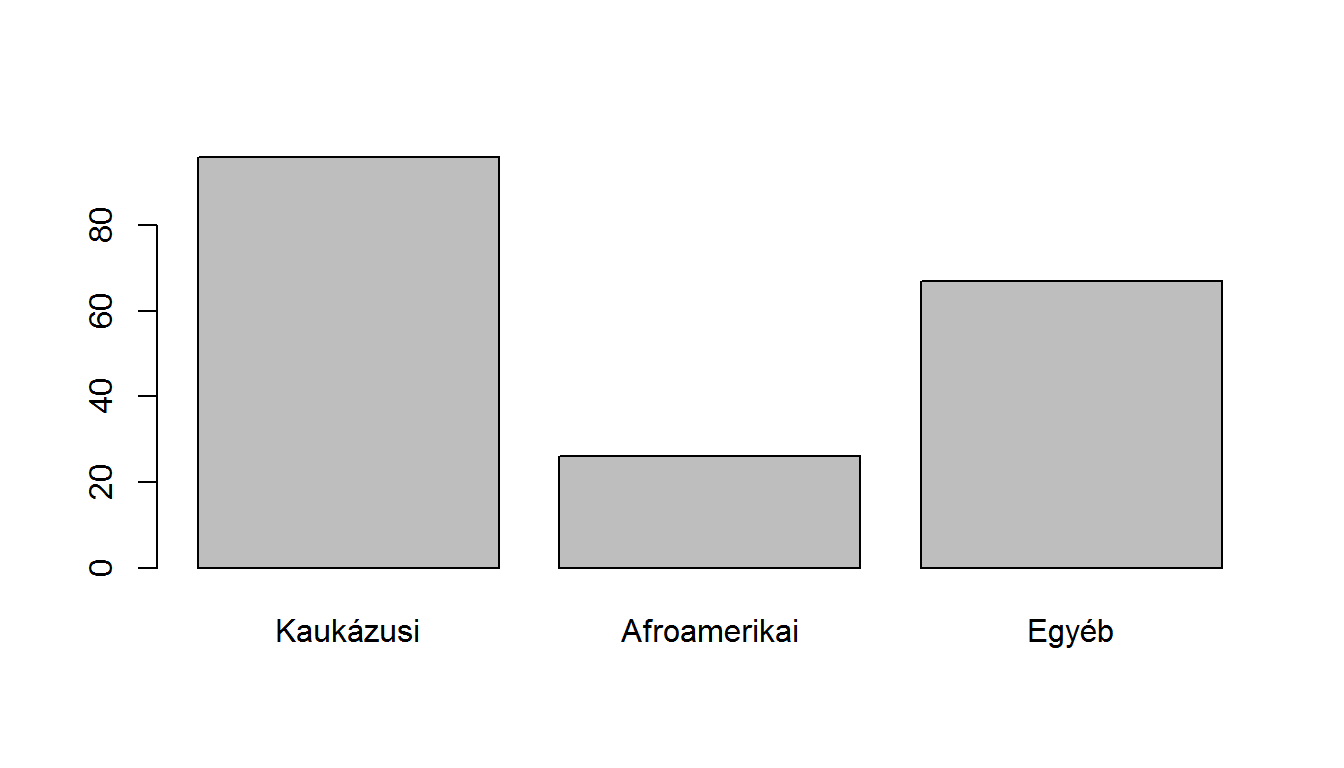
\includegraphics{bevbiostat_files/figure-latex/oszlopdiagram-1.pdf}
\caption{\label{fig:oszlopdiagram}Példa egy minőségi változó ábrázolására
oszlopdiagrammal.}
\end{figure}

Az oszlop- és kördiagramok használata kapcsán megjegyzendő, hogy
tudományos munkákban általában az oszlopdiagram a preferált,
pszichológiai vizsgálatok szerint ugyanis az emberi szem jobban tud
lineáris mértékeket kezelni és értelmezni, mint területet. Az egyetlen
megfontolás, ami mégis az oszlopdiagram ellen szólhat néha, hogy az
oszlopok kirajzolási sorrendje már implikál egyfajta sorrendezést (a
természetes balról-jobbra olvasás miatt), ami adott esetben nem
következik az változó tartalmából.

Az ordinalitás e téren nem sok változást okoz: az oszlopok sorrendje
kötött lesz, illetve ábrázolhatóvá válik a kumulált gyakoriság is
(természetesen csak oszlopdiagrammal).

\section{Mennyiségi változó egyváltozós
elemzése}\label{deskriptivmennyegyvalt}

Mennyiségi változóra jó példa adatbázisunk születési tömeg
(\texttt{bwt}) változója, mely az alany születési tömegét adja meg (és
így arányskálán mért, egész pontosan).

\subsection{Analitikus eszközök}\label{deskriptivmennyegyvaltanalitikus}

Az analitikus eszközök közül először most is a gyakorisági sort, majd a
különböző mutatószámokat tárgyaljuk meg.

\subsubsection{Gyakorisági
sor}\label{deskriptivmennyegyvaltanalitikusgyakorisagisor}

Gyakorisági sor természetesen mennyiségi változóra is készíthető, de
csak módosításokkal. Annak ugyanis, hogy megszámoljuk, hogy az egyes
előforduló kimenetekből mennyi van, nincs sok értelme (hogy egy példával
illusztráljuk: az itt tipikus folytonos változóknál könnyen lehet, hogy
minden egyes előforduló kimenetből csak egyetlen egy lesz). A problémát
nyilván a folytonosság jelenti, ami ellen úgy védekezhetünk, hogy nem
adott értéket felvev\} megfigyelési egységek számát adjuk meg, hanem
\emph{adott intervallumba esőek} számát. Így kapjuk az
\textbf{osztályközös gyakorisági sort}. (Az elnevezés arra utal, hogy
osztályközöket hozunk létre -- így fogjuk hívni az előbb említett
intervallumokat.) A gyakoriság, relatív gyakoriság, kumulált gyakoriság
és kumulált relatív
gyakoriság\footnote{Emlékezzünk vissza, hogy a magasabb mérési skála minden alacsonyabb tulajdonságával bír, így természetesen az összes, alacsonyabb mérési skálán értelmezett módszer a magasabb mérési skálák esetében is alkalmazható.}
értelmezése változatlan. A születési tömeg változó osztályközös
gyakorisági sora (precízebben szólva: egy lehetséges osztályközös
gyakorisági sora; hiszen ez már függeni fog az osztályközök
megválasztásától is), a következő:

\begin{Shaded}
\begin{Highlighting}[]
\NormalTok{tab <-}\StringTok{ }\KeywordTok{table}\NormalTok{(}\KeywordTok{cut}\NormalTok{(birthwt}\OperatorTok{$}\NormalTok{bwt, }\KeywordTok{seq}\NormalTok{(}\DecValTok{500}\NormalTok{, }\DecValTok{5000}\NormalTok{, }\DecValTok{500}\NormalTok{)))}
\KeywordTok{data.frame}\NormalTok{(}\DataTypeTok{Ci0 =} \KeywordTok{seq}\NormalTok{(}\DecValTok{500}\NormalTok{, }\DecValTok{4500}\NormalTok{, }\DecValTok{500}\NormalTok{), }\DataTypeTok{Ci1 =} \KeywordTok{seq}\NormalTok{(}\DecValTok{1000}\NormalTok{, }\DecValTok{5000}\NormalTok{, }\DecValTok{500}\NormalTok{), }\DataTypeTok{fi =}\NormalTok{ tab, }
    \DataTypeTok{gi =} \KeywordTok{prop.table}\NormalTok{(tab))}
\end{Highlighting}
\end{Shaded}

\begin{verbatim}
##    Ci0  Ci1         fi.Var1 fi.Freq         gi.Var1 gi.Freq
## 1  500 1000     (500,1e+03]       1     (500,1e+03]   0,005
## 2 1000 1500 (1e+03,1,5e+03]       4 (1e+03,1,5e+03]   0,021
## 3 1500 2000 (1,5e+03,2e+03]      14 (1,5e+03,2e+03]   0,074
## 4 2000 2500 (2e+03,2,5e+03]      40 (2e+03,2,5e+03]   0,212
## 5 2500 3000 (2,5e+03,3e+03]      38 (2,5e+03,3e+03]   0,201
## 6 3000 3500 (3e+03,3,5e+03]      45 (3e+03,3,5e+03]   0,238
## 7 3500 4000 (3,5e+03,4e+03]      38 (3,5e+03,4e+03]   0,201
## 8 4000 4500 (4e+03,4,5e+03]       7 (4e+03,4,5e+03]   0,037
## 9 4500 5000 (4,5e+03,5e+03]       2 (4,5e+03,5e+03]   0,011
\end{verbatim}

Itt \(C_{i0}\) és \(C_{i1}\) az \(i\)-edik osztályköz alsó és felső
határát jelöli, rendre. (Az megállapodás kérdése, hogy a határon lévő
megfigyelési egységeket, például egy pont 2000 grammos újszülöttet hová
sorolunk, ennek természetesen csak a kerekítésből adódó diszkrétség
miatt van egyáltalán jelentősége.)

Vegyük észre, hogy ez a megoldás lényegében azt jelenti, hogy a
mennyiségi változónkat első lépésben ,,lefokozzuk'' minőségi változóvá,
és utána alkalmazzuk -- mint teljesen közönséges minőségi változóra -- a
korábban megismert módszert.

Elöljáróban jegyezzük meg, hogy itt már a gyakorisági sor -- szemben a
minőségi esettel -- igenis információvesztéssel jár: lehet 14 újszülött
1501 grammos, és lehet mind a 14 1999 grammos, mindkét esetben ugyanúgy
a fenti osztályközös gyakorisági sort kapjuk. Az információvesztés
mértékét nyilván az osztályközök hossza (a felosztás ,,finomsága'')
fogja meghatározni.

A sor előtti zárójeles megjegyzésünk már utal arra, hogy mi az
osztályközös gyakorisági sorok használatának legnagyobb kihívása: az
osztályközök helyes megválasztása. Az információveszteség minimalizálása
szempontjából nyilván a minél szűkebb osztályközök a jobbak, viszont
túlzásba ezt sem lehet vinni, különben értelmét veszti az egész eszköz,
azáltal, hogy megszűnik a lényegkiemelő jelleg. (Ha egyre jobban és
jobban szűkítjük az osztályközöket, akkor egy idő után visszajutunk oda,
hogy az intervallumok túlnyomó részében 0 lesz a gyakoriság, a többiben
pedig 1-1 -- azaz lényegében visszakapjuk a minta ,,felsorolását''.) Az
egyetlen dolog, ami univerzálisan segít ezen, az a mintanagyság növelése
(hiszen lehetővé teszi az osztályközök szűkítését úgy, hogy közben
várhatóan nem csökken az egy osztályközbe eső megfigyelési egységek
száma).

Ráadásul az osztópontok megválasztása nem csak az információveszteség
szempontjából fontos. Az, hogy a gyakorisági sor milyen képest sugall
számunkra a vizsgált változóról -- sajnos -- nagyban változhat akár az
osztópontok nem túl lényeges áthelyezésének hatására is, különösen kis
mintanagyságnál. Éppen ezért jelent a gyakorlatban komoly kihívást az
osztályközök határainak jó megválasztása.

Hogy ezt hogyan tegyük meg, arra alapvetően két lehetőségünk van. Az
egyik út az, hogy tárgyterületi információkat használunk fel, azaz
megpróbálunk -- az adott változó jelentését is figyelembe véve --
szakmailag értelmes, tartalommal bíró osztópontokat találni. (A fenti
gyakorisági sor példa erre, hiszen kerek, emberi szem számára
kényelmesen értelmezhető osztópontokat vettünk fel.) A másik lehetőség,
hogy tisztán statisztikai alapon (tehát a változó tárgyterületi
jelentésének felhasználása nélkül) döntünk -- vannak módszerek, melyek
pusztán a megfigyelések statisztikai jellemzői (nagyság, szóródás stb.)
alapján igyekeznek ,,kitalálni'', hogy hová érdemes rakni az
osztópontokat ahhoz, hogy a lehető leginformatívabb gyakorisági sort
kapjuk. Példának okáért, az egyik ilyen ismert analitikus szabály a
Sturges-szabály, ami azt javasolja, hogy
\(\left\lceil \log_2 n+1\right\rceil\) darab azonos szélességű
osztályközt vegyünk fel a mintaminimum és -maximum között.

\subsubsection{Mutatószámok}\label{deskriptivmennyegyvaltanalitikusmutatoszamok}

A mutatószámok a megfigyelések valamilyen jellemzőjét próbálják meg
egy-egy számba tömörítve megragadni. A következőkben aszerint
csoportosítva mutatjuk be őket, hogy mi ez a megragadott jellemző.

\paragraph{Középértékek (centrális
tendencia)}\label{deskriptivmennyegyvaltanalitikusmutatoszamokcentralistendencia}

\textbf{Centrális tendencia} alatt azt értjük, hogy mi az az érték, ami
körül csoportosulnak a megfigyelések. Függően a konkrét mutatótól,
olyanokra gondolhatunk ez alatt, mint ,,közepes'`, ,,tipikus'`vagy
,,átlagos'' érték. A legtöbb statisztikai alkalmazás szempontjából ez a
legfontosabb jellemzője a változónak, ezért ha csak egyetlen számmal
jellemezhetjük a változót, az tipikusan a centrális tendencia valamilyen
leírója lesz. Ezeket a mutatószámokat általában \textbf{középértéknek}
vagy \textbf{helyzetmutatónak} nevezik.

A centrális tendencia legismertebb mutatója a \textbf{(számtani) átlag},
jele \(\overline{x}\). Definíciószerűen nem más, mint az az szám, amivel
helyettesítve minden megfigyelési egység értékét, az ún. értékösszeg (a
változó megfigyeléseinek összege) változatlan maradna: \[
    \overline{x}=\frac{\sum_{i=1}^n x_i}{n}.
\]

Azonnal látható, hogy ennek akkor van értelme, ha a különböző
megfigyelések számtani összege valamilyen értelmes tartalommal bír. (Van
például értelme beszélni egy osztály átlagos testtömegéről, hiszen a
testtömegek összege értelmes kifejezés, megadja például, hogy mennyit
mutatna egy mérleg, ha mindenki ráállná.) Ha azonban a változó olyan,
hogy nem az megfigyelések összegének van értelme, akkor a számtani átlag
használata félrevezető lehet, és mással kell helyettesíteni -- például,
ha a megfigyelések összege helyett azok szorzata a tárgyterületileg
értelmes, akkor az ún. mértani átlaggal. (Tipikus példa erre az, ha a
változó valamilyen növekedési ütemet jelent időben. Ha egy alany
testtömege egy évben 1,2-szeresére nőtt, rákövetkező évben pedig
1,3-szeresére, akkor az össznövekedés nyilván nem a növekedések összege
(\(1,\!2 + 1,\!2 = 2,\!4\)), hanem azok szorzata
(\(1,\!2 \cdot 1,\!2 = 1,\!44\)) lesz.)

A születési tömegek átlaga 2944,6 gramm, ami azt jelenti, hogy az
adatbázisban szereplő újszülöttek össz-testtömege akkor maradna
változatlan, ha mindegyikük 2944,6 gramm lenne.

Az átlag ún. számított középérték, mivel valamilyen számszerű
összefüggésben van a megfigyelések értékeivel.

Az átlag előnye, hogy rendkívül közismert, mindenki számára kényelmesen
kezelhető, szokásos gondolkodásunkhoz közel álló mutató. (Ez olyannyira
erős tényező, hogy nagyon sok orvosi publikáció még akkor is erőlteti az
átlag használatát, amikor az -- a mindjárt részletezendő okokból -- nem
célszerű.)

Az átlag legnagyobb hátránya, hogy nem \textbf{robusztus}. Egy
statisztikai mutatószám robusztussága azt méri, hogy mennyire érzékeny
arra, ha a mintában a többi értéktől, a csoportosulás alaptendenciájától
jelentősen eltérő érték vagy értékek vannak. Az ilyen megfigyeléseket
egyébként nagyon gyakran \textbf{outliernek} is nevezik.
(,,Érzékenység'`alatt azt értjük, hogy a mutatót mennyire tudja
befolyásolni, eredeti értékétől eltéríteni ilyen outlierek jelenléte.)
Az átlag ilyen szempontból extrém rossz mutató: egyrészt bármelyik
megfigyelés bármilyen megváltozása módosítja az átlag értékét, de ami az
igazán nagy baj, hogy ha egyetlen megfigyelés is tart a végtelenhez, úgy
az átlag is tart a végtelenhez, \emph{függetlenül} az összes többi
megfigyeléstől, és függetlenül a minta nagyságától. Mindez azt mondja
nekünk, hogy ha csak egyetlen outlier is van a mintában, már az is képes
arra, hogy teljesen értelmetlenné tegye az átlagot. (Hiszen ha van egy
ilyen outlier a mintában, akkor az átlag \emph{pont hogy nem} a minta
,,közepes'' értékét fogja mutatni, hanem egyre inkább az outlierét,
minél jobban kilóg.)

Megjegyezzük, hogy pontosan emiatt az átlag használata a centrális
tendencia jellemzésére nem csak gyakorlati szempontból lehet problémás
(adatrögzítési hibákból, adatbázis-sérülésekből eredeti outlierek),
hanem elméletileg is ellenjavallt, ha a változó olyan, hogy fel kell
készülni kis számú, de a többitől lényegesen nagyobb vagy kisebb
megfigyelés jelenlétére. (Ez fordulhat elő -- mindenféle adatrögzítési
és egyéb hiba nélkül is! -- például ún. aszimmetrikus eloszlásoknál,
melyekről később fogunk részletesebben beszélni.)

Épp ezen a robusztussági problémán igyekszik javítani a \textbf{trimmelt
(vagy nyesett) átlag}: ezt úgy kapjuk, hogy elhagyjuk a legkisebb és
legnagyobb adott számú elemet, és csak a maradékot átlagoljuk ki.
Tipikusan az elhagyott megfigyelések száma alul és felül is a
mintanagyság 2,5\%-a; ebben az esetben 5\%-os trimmelt átlagról
beszélünk. (Bár elsőre ez szokatlan mutatónak tűnhet, és a tudományos
irodalomban tényleg ritkábban is használják, de számos pontozásos
sportágban épp ilyen elven alakítják ki a zsűri ,,átlagos'' pontszámát.)
A születési tömegek 5\%-os trimmelt átlaga 2957,4 gramm, ami egyúttal
azt is mutatja, lévén, hogy közel van a szokásos átlaghoz, hogy a
születési tömegek aránylag szimmetrikus eloszlásúak, vélhetően komoly
outlier nélkül.

Alapvetően más megközelítését jelenti a centrális tendencia
megragadásának a \textbf{medián} használata, melynek jele
\(\mathrm{Me}_x\). A medián nem más, mint a nagyság szerint
sorbarendezett megfigyelések közül a középső. (Amennyiben a mintanagyság
páros, úgy nyilván két ,,középső'' is van, ez esetben megállapodás
kérdése, hogy mit nevezünk mediánnak; vehetjük például a kettő átlagát.)
Úgy is szoktak fogalmazni, hogy a medián felezőpont, az az érték, amiről
elmondható, hogy alatta és felette is egyaránt ugyanannyi mintaelem (az
összes fele-fele) található.

Értelemszerű, hogy a medián szintén a centrális tendenciát jellemzi,
csak épp kevésbé megszokott módon, mint az átlag -- ez egyúttal
használatának egyik fő gátja is: sok ember számára a medián tartalma (és
egyáltalán, értelme) kevésbé ismert, így e mutató nem annyira jól
kezelhető. Előnye viszont a robusztusság, ilyen szempontból az átlaggal
szemben a másik végpontot képviseli: míg az átlag extrém érzékeny volt,
addig a medián extrém robusztus. A minta minden medián feletti értéke
(az egyszerűség kedvéért most gondoljunk páratlan mintanagyságra)
tetszőlegesen megnövelhető (akár az összes egyszerre is), vagy a medián
alatti értékek tetszőlegesen lecsökkenthetőek (akár az összes egyszerre
is), vagy akár a kettő együtt is, a medián értéke \emph{nem változik}!
Hátránya, hogy a jó robusztusságért cserében kevesebb információt
használ fel a
mintából\footnote{Így már az is érthető, hogy a trimmelt átlag egyfajta kompromisszumnak tekinthető a kettő között, ti. a robusztusság és a mintaértékek mind teljesebb kihasználása között. Az is észrevehető, hogy bizonyos értelemben ez ráadásul általánosítja is a két mutatót: a 0\%-os trimmelt átlag épp a ,,hagyományos'' átlag, a 100\%-os trimmelt átlag pedig épp a medián.};
ezt épp a mintaértékek meglehetősen szabad ,,állítgathatósága'' mutatja.
(Hogy ez miért baj, az precízen csak induktív statisztikai keretben
lehet megérteni, az ottani tárgyalás után már érthető lesz, hogy mit
jelent az, hogy a medián kevésbé hatásos becslő mint az átlag.) A
tanulság az, hogy ha feltehető, hogy a háttéreloszlás
szimmetrikus-közeli, akkor érdemes átlagot használni, ha nem, vagy
outlierek jelenlétére is fel kell készülni (azaz indokolt robusztus
statisztika használata), akkor jobb a medián ilyen szempontból.

A születési tömegek mediánja 2977 gramm, azaz a 2977 gramm az a
testtömeg, amiről elmondható, hogy az újszülöttek fele kisebb ennél,
fele nagyobb.

Ahogy a medián a minta ,,felezőpontja'' ugyanúgy definiálhatók általános
osztópontok; ezeket \textbf{kvantiliseknek} nevezzük. A \(p\)-kvantilis
(\(0<p<1\)) az az érték, amiről elmondható, hogy a megfigyelések
\(p\)-ed része kisebb nála, \(\left(1-p\right)\)-ed része nagyobb nála.
(Tehát a medián az \(1/2\)-kvantilis.) Gyakorlati szempontból nagyobb
jelentősége van még a negyedelőpontoknak, melyek neve
\textbf{kvartilis}. Ilyenből tehát nyilván három van: a
\(p=1/4,2/4=1/2,3/4\)-kvantilis, ezek közül a középső persze ugyanaz
mint a medián. A másik kettőt alsó és felső kvartilisnek szokták
nevezni, és \(Q_1\)-gyel, illetve \(Q_3\)-mal jelölik. Tehát például
\(Q_1\) az a szám, amire igaz, hogy a minta egynegyede (darabszámra)
nála kisebb értékű, háromnegyede nála nagyobb. Ezek valójában már nem is
a centrális tendenciát, hanem általában az eloszlás alakját mutatják,
mégpedig robusztus módon (ugyanazon okból, mint amit a mediánnál is
láttunk). Ritkábban, de szokták használni ugyanerre a célra a
tizedelőpontokat, nevük decilis (\(D_1,D_2,\ldots,D_9\)) és a
századolópontokat, nevük percentilis (\(P_1,P_2,\ldots,P_{99}\)).

A módusz használatának a folytonosság miatt általában nincs értelme
mennyiségi változó esetén, ahogy azt már említettük is. Értelmet csak az
ad neki, ha diszkretizáljuk (csoportosítjuk) az adatokat, ahogy az a
gyakorisági sorral történt is. Ilyenkor már van értelme móduszról
beszélni, persze ekkor már csak osztályköz szintjén -- szokás ezt
\textbf{modális osztályköznek} is nevezni. Például a születési tömegek
fent közölt osztályközös gyakorisági sorában (ne feledjük, itt már az is
számít, hogy melyik osztályközös gyakorisági sorra vonatkozóan adjuk
meg!) a modális osztályköz a 3000--3500 gramm.

A módusz és a medián ún. \textbf{helyzeti középérték}, mivel nem
számítás eredményeként adódnak, hanem a többi megfigyeléshez képest
elfoglalt helyzetük tünteti ki őket.

Ennek kapcsán azt is megjegyezzük, hogy átlagot, mediánt (és általában
minden egyéb mutatószámot is) lehetséges osztályközös gyakorisági sorból
(a nyers mintaelemek ismerete nélkül is) számolni, persze ekkor már csak
közelítő jelleggel.

\paragraph{Szóródás}\label{deskriptivmennyegyvaltanalitikusmutatoszamokszorodas}

\textbf{Szóródásnak} nevezzük azt, hogy a megfigyelések milyen szorosan
csoportosulnak azon érték körül, ami körül csoportosulnak (lásd a
centrális tendenciát!), más szóval mennyire ingadoznak a megfigyelések,
mekkora változékonyság van bennük. A gyakorlatban ez a második
legfontosabb kérdés: ha csak egy jellemzőt adhatunk meg, akkor az a
centrális tendencia lesz, de ha kettőt, akkor megadjuk azt is, hogy
mekkora a szóródás.

A minta szóródásának legegyszerűbb mérőszáma a legkisebb
(\(\mathrm{Min}\)) és a legnagyobb (\(\mathrm{Max}\)) mintaelem értéke,
a \textbf{mintaminimum} és \textbf{mintamaximum}, illetve kettejük
különbsége, melyet \textbf{terjedelemnek} nevezünk és \(R\)-rel
jelölünk: \(R=\mathrm{Max}-\mathrm{Min}\). Ezek előnye, hogy teljesen
egyértelmű a tartalmuk, hátrányuk, hogy rendkívül érzékenyek arra, hogy
konkrétan milyen mintát vettünk a sokaságból, ezért következtetési
célokra nem is szokták alkalmazni.

A születési tömegek mintaminimuma 709 gramm, mintamaximuma 4990 gramm,
így e változó terjedelme 4281gramm.

A leggyakoribb általános célú mutatója a szóródásnak a \emph{szórás},
jele általában \(s_x\) vagy \(\sigma_x\). (A kettő neve nem keverendő: a
,,szóródás'`a jellemző, a ,,szórás'' egy lehetséges mutatószáma a
szóródásnak.) A szórás nem más, mint a megfigyelések átlagtól vett
átlagos eltérése. Ez utóbbi átlag alatt négyzetes átlagot értve --
egyszerű számtani átlag nem lenne jó, hiszen azzal a pozitív és negatív
irányú eltérések csökkentenék (sőt, belátható, hogy kioltanák) egymás
hatását. Azaz: \[
    s_x=\sqrt{\frac{\sum_{i=1}^n \left(x_i-\overline{x}\right)^2}{n}}.
\]

Ennek a négyzetét szokás szórásnégyzetnek vagy \textbf{varianciának}
nevezni. Deskriptív esetben néha inkább mintaszórást illetve
mintavarianciát mondanak (hogy a megfelelő valószínűségszámítási
fogalomtól megkülönböztessék).

A fent definiált mutatót szokás precízen korrigálatlan mintaszórásnak
nevezni, ezzel szemben a \textbf{korrigált mintaszórás}: \[
    s_x^{\ast}=\sqrt{\frac{\sum_{i=1}^n \left(x_i-\overline{x}\right)^2}{n-1}}.
\] A különbségük oka csak a következtető statisztikában válik világossá
(a korrigálatlan mintavariancia, első ránézésre talán meglepő módon, nem
torzítatlan becslője a sokasági varianciának).

A születési tömegek korrigált mintaszórása 729,2 gramm, tehát az
újszülöttek testtömegeinek átlaguk körül vett ingadozásának (négyzetes)
átlaga 729,2 gramm.

A szórás hátránya, hogy -- az átlaghoz hasonlóan -- nem robusztus
mutató. (Egyrészt azért, mert maga is az eltérések négyzetét használja,
ami érzékeny a kilógó értékekre, másrészt azért, mert a eltéréseket a
nem-robusztus átlagtól veszi.) Egyik lehetséges megoldás az
\textbf{interkvartilis terjedelem} (jele \(IQR\)) használata, ami a
felső és az alsó kvartilis különbsége: \[
    IQR=Q_3-Q_1.
\] Az interkvartilis terjedelem a robusztus kvartiliseken alapul, így
robusztus mutató, és könnyen látható, hogy tartalmilag a szóródást
jellemzi, hiszen minél jobban szóródott az eloszlás, annál távolabb lesz
az alsó és a felső negyedelőpontja.

A születési tömegek interkvartilis terjedelme 1073 gramm, tehát az a
tömeg, ami fölött az újszülöttek egynegyede (és alatta háromnegyede)
van, 1073 grammal nagyobb annál a tömegnél, ami fölött az újszülöttek
háromnegyede (és alatta egynegyede) van.

A másik lehetőség a szórás ,,megjavítása'`, olyan módon, hogy az
eltéréseknek nem a négyzetét, hanem az abszolút értékét vesszük. (Ezzel
a kapott mennyiség matematikai kezelhetőségét rontjuk, hiszen a
négyzetreemelés jobban kezelhető matematikai objektum, de a
robusztusságot növeljük.) További javítási lehetőség, ha az eltéréseket
nem az átlagtól hanem a mediántól vesszük, és nem is átlagoljuk őket,
hanem a mediánjukat képezzük. A mutató neve, ami mindhárom ,,trükköt''
beveti: \textbf{medián abszolút eltérés}, jele \(MAD\), tehát \[
    MAD=\mathrm{Me}\left(\left|x_i-\mathrm{Me}\left(x\right)\right|\right).
\] (A szakirodalom itt nem teljesen egyértelmű: néha \(MAD\)-nak nevezik
azt a mutatót is, ahol csak az első javítást csinálják meg, tehát
abszolútértéket vesznek, de azokat továbbra is csak átlagolják, és az
eltéréseket is az átlagtól veszik.)

A születési tömegek medián abszolút eltérése 834,7 gramm, tehát az
újszülöttek testtömegeinek mediánjuk körül vett (abszolút) ingadozásának
mediánja 834,7 gramm. (Pontosabban szólva ezek az értékek a fent
definiált \(MAD\) 1,4826-szorosai, a konstans szorzó értelme, hogy így a
normális eloszlás \(MAD\)-ja épp a szórás lesz.)

\paragraph{Alakmutatók}\label{deskriptivmennyegyvaltanalitikusmutatoszamokalakmutatok}

A fenti két jellemzőn túlmenően néha egyéb, még inkább részletekbe menő
jellemzőit is használják egy változó leírásának. Egy tipikus példa erre
a \textbf{szimmetria}: egy eloszlás szimmetrikus, ha a centrális
tendencia helyétől mindkét irányban nagyjából hasonló a lefutása.
(Vegyük észre, hogy ez nem következik még abból sem, ha két változóra
ugyanaz a centrális tendencia, és ugyanaz a szóródás: ettől még az egyik
lehet szimmetrikus, míg a másik nem.) A nem szimmetrikus eloszlásokat
szokás \textbf{ferde} eloszlásoknak is nevezni; ezen belül is szoktak
balra ferde (jobbra hosszan elnyúló) és jobbra ferde (balra hosszan
elnyúló) eloszlásról beszélni, attól függően, hogy melyik irányban
nagyobb a szóródás. További kérdések is felmerülnek, mint a csúcsosság,
a multimodalitás stb. -- ezekkel és a továbbiakkal azonban részletesen
itt nem foglalkozunk.

\subsection{Grafikus eszközök}\label{deskriptivmennyegyvaltgrafikus}

A grafikus eszközök közül először a hisztogramot, utána röviden a
magfüggvényes sűrűségbecslőt, majd végül a boxplotot tárgyaljuk meg.

\subsubsection{Hisztogram}\label{deskriptivmennyegyvaltgrafikushisztogram}

A hisztogram leegyszerűsítve nem más, mint az osztályközös gyakorisági
sor ábrázolása oszlopdiagramon, annyi specialitással, hogy az oszlopokat
közvetlenül egymás mellé rajzoljuk, hely kihagyása nélkül
(\ref{fig:hisztogram}. ábra).

\begin{Shaded}
\begin{Highlighting}[]
\KeywordTok{hist}\NormalTok{(birthwt}\OperatorTok{$}\NormalTok{bwt, }\DataTypeTok{xlab =} \StringTok{"Születési tömeg [g]"}\NormalTok{, }\DataTypeTok{ylab =} \StringTok{"Gyakoriság"}\NormalTok{, }\DataTypeTok{main =} \StringTok{""}\NormalTok{)}
\KeywordTok{rug}\NormalTok{(birthwt}\OperatorTok{$}\NormalTok{bwt)}
\end{Highlighting}
\end{Shaded}

\begin{figure}
\centering
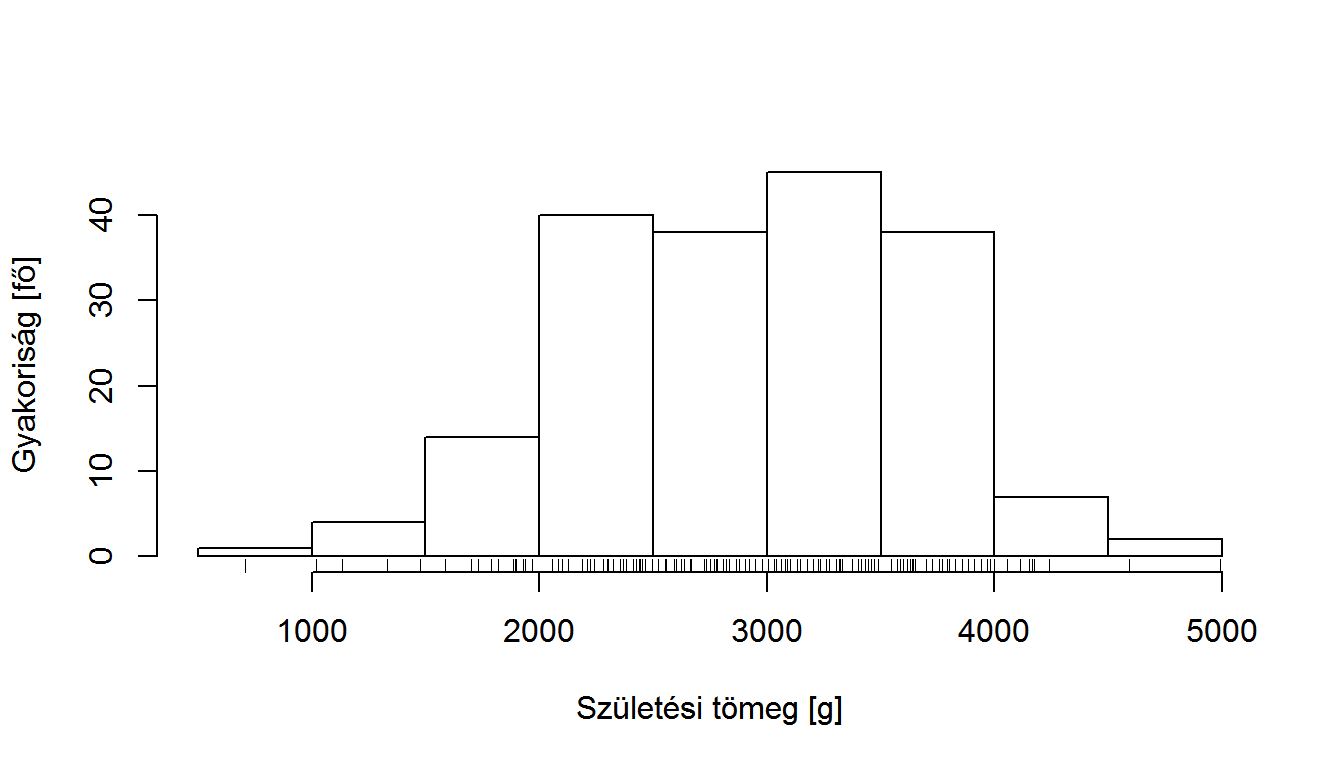
\includegraphics{bevbiostat_files/figure-latex/hisztogram-1.pdf}
\caption{\label{fig:hisztogram}Példa egy mennyiségi változó ábrázolására
hisztogrammal.}
\end{figure}

Az ábrán látható, hogy az oszlopok határai kijelölik az osztályközöket
(ezek természetesen nem feltétlenül azonos szélességűek); adott
osztályköz fölé pedig \[
    \frac{f_i}{n \cdot h_i}
\] magasságú oszlopokat rajzolunk, ahol \(h_i\) az adott osztályköz
szélessége. Ezen az ábrán feltüntettük (alul, apró tüskékként) magukat a
nyers megfigyeléseket is (,,rugplot'').

A hisztogram a legnépszerűbb adatvizualizációs módszer mennyiségi
változókra. Ahogy már utaltunk is rá, hatalmas előnye, hogy a vizuálisan
közölt információ rendkívül jól feldolgozható az emberi agy számára: a
fenti hisztogram alapján szinte ,,ránézésre'', egyetlen pillantással jó
képünk alakul ki a centrális tendenciáról, a szóródásról, sőt, az
eloszlás alakjának finomabb jellemzőiről is. Egy átlagot még el sem
olvastunk, amikorra a hisztogram alapján már olyan finom jellemzőkről,
mint az eloszlás szimmetriája is képünk van.

Hátránya, hogy kevésbé objektív (mint a grafikus módszerek általában) --
ha például két változót össze kell hasonlítanunk, akkor két átlaggal
(azaz két számmal) az értelemszerűen könnyebben megtehető mint két
hisztogrammal.

A legnagyobb kihívás azonban az osztályközök helyes megválasztása. Ez a
probléma teljesen ugyanaz, mint amit az osztályközös gyakorisági sornál
is kifejtettünk. Sőt, itt talán még jobban szemléltethető: a következő
ábrán ugyanazt az adatsort ábrázoltuk, csak épp az optimálisnál
lényegesen több, illetve lényegesen kevesebb osztályközt használva is
(\ref{fig:hisztogramvalasztasok}. ábra).

\begin{Shaded}
\begin{Highlighting}[]
\KeywordTok{par}\NormalTok{(}\DataTypeTok{mfrow =} \KeywordTok{c}\NormalTok{(}\DecValTok{1}\NormalTok{, }\DecValTok{3}\NormalTok{))}
\KeywordTok{hist}\NormalTok{(birthwt}\OperatorTok{$}\NormalTok{bwt, }\DecValTok{3}\NormalTok{, }\DataTypeTok{xlab =} \StringTok{"Születési tömeg [g]"}\NormalTok{, }\DataTypeTok{ylab =} \StringTok{"Gyakoriság"}\NormalTok{, }\DataTypeTok{main =} \StringTok{""}\NormalTok{)}
\KeywordTok{hist}\NormalTok{(birthwt}\OperatorTok{$}\NormalTok{bwt, }\DataTypeTok{xlab =} \StringTok{"Születési tömeg [g]"}\NormalTok{, }\DataTypeTok{ylab =} \StringTok{"Gyakoriság"}\NormalTok{, }\DataTypeTok{main =} \StringTok{""}\NormalTok{)}
\KeywordTok{hist}\NormalTok{(birthwt}\OperatorTok{$}\NormalTok{bwt, }\DecValTok{30}\NormalTok{, }\DataTypeTok{xlab =} \StringTok{"Születési tömeg [g]"}\NormalTok{, }\DataTypeTok{ylab =} \StringTok{"Gyakoriság"}\NormalTok{, }\DataTypeTok{main =} \StringTok{""}\NormalTok{)}
\end{Highlighting}
\end{Shaded}

\begin{figure}
\centering
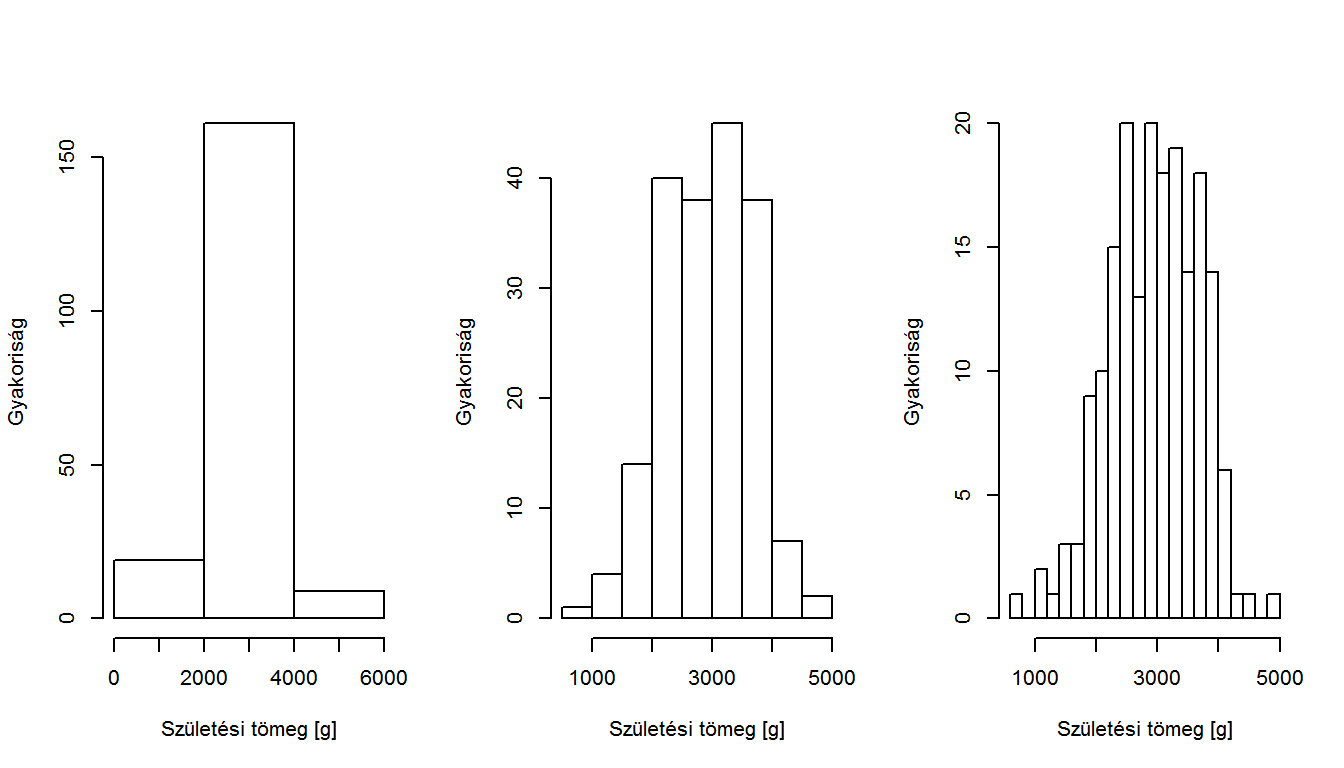
\includegraphics{bevbiostat_files/figure-latex/hisztogramvalasztasok-1.pdf}
\caption{\label{fig:hisztogramvalasztasok}Ugyanazon adatsor ábrázolása
különféle számú osztályközt tartalmazó hisztogrammal.}
\end{figure}

Itt érzékelhető igazán, hogy miért probléma az is, ha túl finom, és az
is, ha túl durva felosztást választunk (adott, rögzített mintanagyság
mellett!). Amennyiben az osztályközök száma túl kevés, akkor sok
információt vesztünk: az eloszlásról kapott kép összemossa a finomabb
részleteket (bal oldal). Úgy is szokták mondani: nagy lesz a torzítás.
Ha viszont túl sok osztályközt választunk, akkor rendkívül esetlegessé
válik, hogy egy osztályközbe hány mintaelem esik, nagyon ingadozó lesz a
magasság (jobb oldal), úgy szokták mondani: nagy lesz a variancia. (Ez
itt a sok más helyen is megjelenő torzítás-variancia trade-off egy
példája.) Ahogy sokszor elmondtuk: valamiféle optimumot kell találni a
kettő között. Ennek módszereiről az osztályközös gyakorisági sornál már
írtunk.

\subsubsection{Magfüggvényes
sűrűségbecslő}\label{deskriptivmennyegyvaltgrafikuskde}

A hisztogrammal kapcsolatos egyik probléma az előbb említett érzékenység
az osztályközök megválasztására. Emellett felvethető az is, hogy a
hisztogram szakaszonként konstans becslést ad, ami zavaró lehet
(különösen, ha kicsi a mintanagyság, és emiatt nem tudunk sok
osztályközt felvenni). Ez utóbbit kiküszöböli, és sok gyakorlati esetben
az előbbit is enyhíti a \textbf{magfüggvényes sűrűségbecslő}
alkalmazása. Ennek matematikai részleteivel most nem foglalkozunk,
megelégszünk annyival, hogy a hisztogramhoz hasonlóan az eloszlás
alakját becsli, ám a hisztogramtól eltérően nem szakaszonként konstans
görbével (\ref{fig:kde}. ábra).

\begin{Shaded}
\begin{Highlighting}[]
\KeywordTok{plot}\NormalTok{(}\KeywordTok{density}\NormalTok{(birthwt}\OperatorTok{$}\NormalTok{bwt), }\DataTypeTok{xlab =} \StringTok{"Születési tömeg [g]"}\NormalTok{, }\DataTypeTok{ylab =} \StringTok{"Sűrűség"}\NormalTok{, }\DataTypeTok{main =} \StringTok{""}\NormalTok{)}
\end{Highlighting}
\end{Shaded}

\begin{figure}
\centering
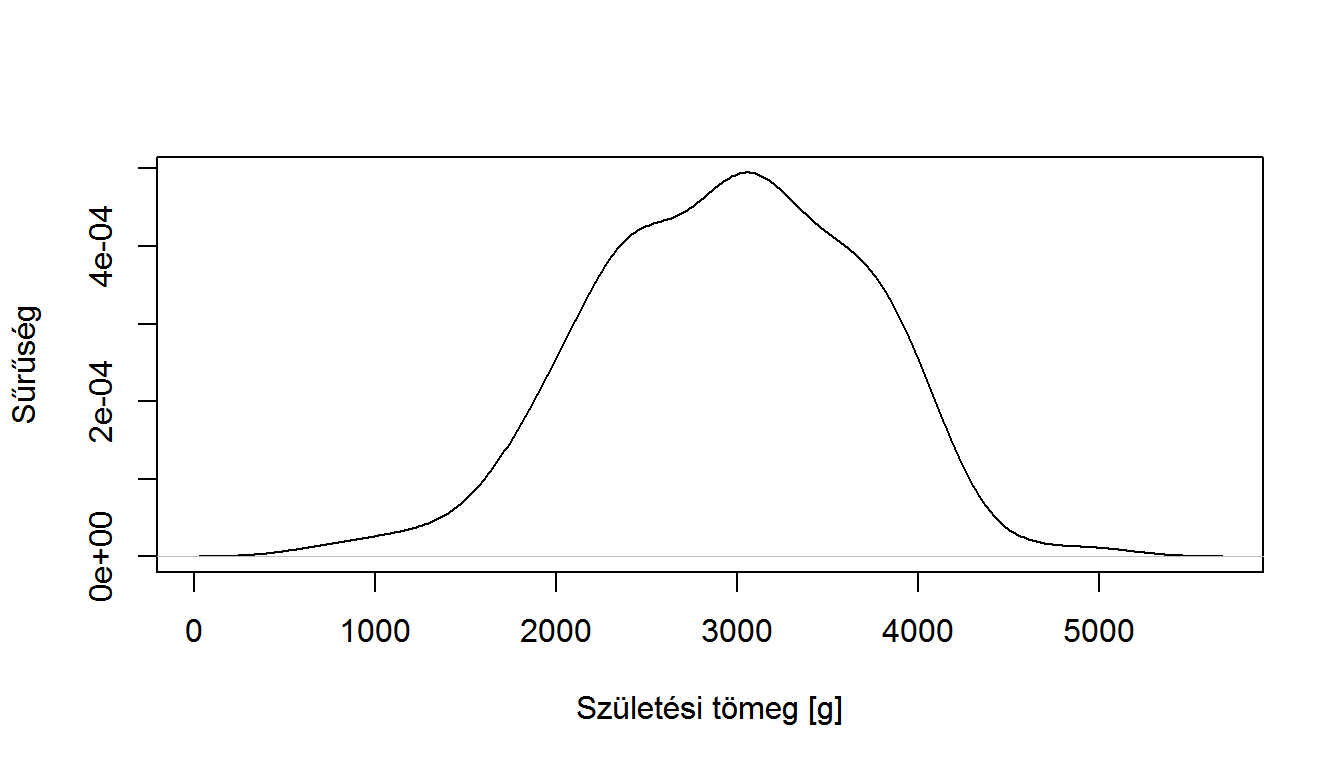
\includegraphics{bevbiostat_files/figure-latex/kde-1.pdf}
\caption{\label{fig:kde}Példa egy mennyiségi változó ábrázolására
magfüggvényes sűrűségbecslővel.}
\end{figure}

Sajnos az osztályközök megválasztásának problémája teljesen nem oldódik
meg, a magfüggvényes sűrűségbecslőnek is van ugyanis állítható
paramétere (magfüggvény, és különösen az ún. sávszélesség). Ennek
optimális megválasztása szintén probléma lehet, különösen, ha nagyon
egyenetlen a mintaelemek eloszlása.

\subsubsection{(Tukey-féle)
boxplot}\label{deskriptivmennyegyvaltgrafikusboxplot}

Végül egy egész más elven felépülő, de szellemes, és a gyakorlatban is
nagyon hasznos vizualizációs módszerrel ismerkedünk meg, a (Tukey-féle)
\emph{boxplottal} (vagy ritkán használt magyar nevén: dobozábrával).

A boxplot nem más, mint egy számegyenes fölé rajzolt téglalap, mely egy
adott változót reprezentál úgy, hogy a téglalap alsó széle az alsó
kvartilisnél (\(Q_1\)-nél), a felső széle pedig a felső kvartilisnél
(\(Q_3\)-nál) van. A téglalapon belül egy vastagabb függőleges vonal is
látható, ez a mediánnál található (\ref{fig:boxplot}. ábra).

\begin{Shaded}
\begin{Highlighting}[]
\KeywordTok{boxplot}\NormalTok{(birthwt}\OperatorTok{$}\NormalTok{bwt)}
\end{Highlighting}
\end{Shaded}

\begin{figure}
\centering
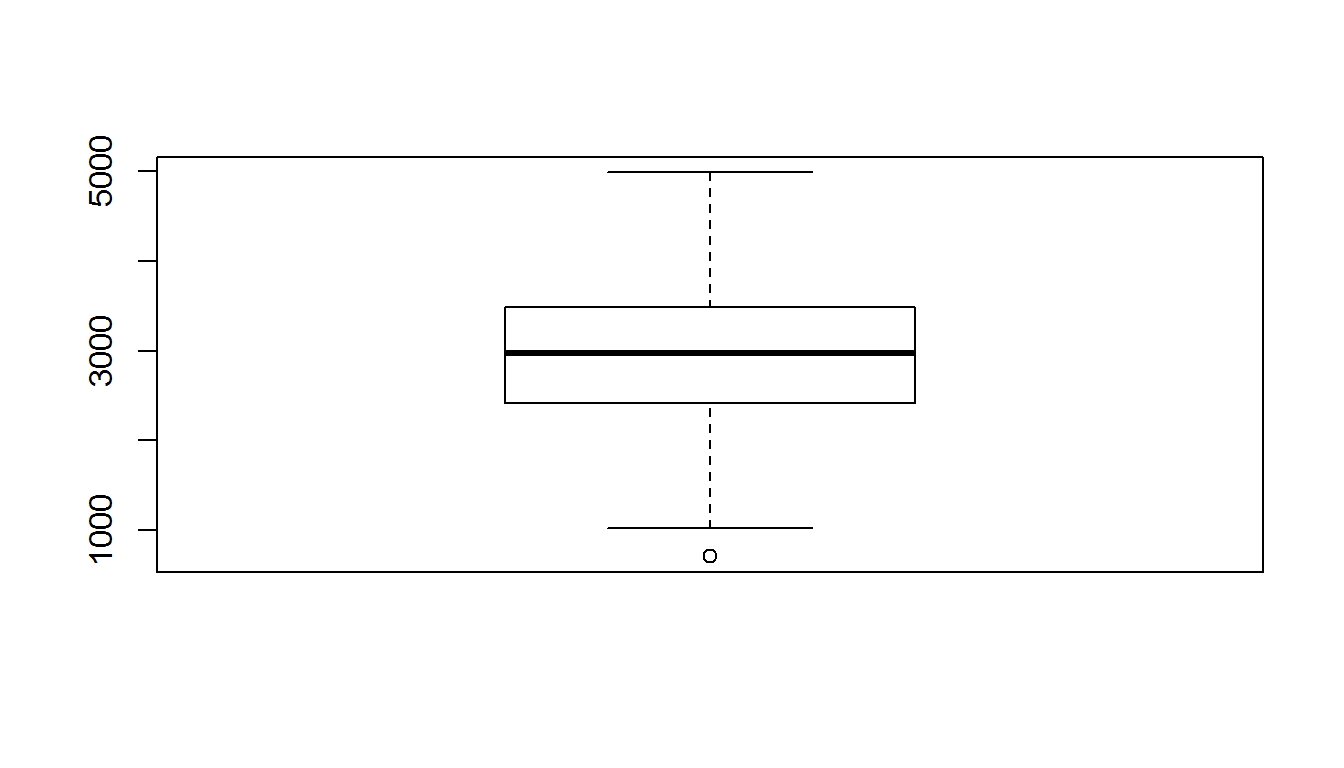
\includegraphics{bevbiostat_files/figure-latex/boxplot-1.pdf}
\caption{\label{fig:boxplot}Példa egy mennyiségi változó ábrázolására
boxplottal.}
\end{figure}

A boxplotból két ,,antenna'' nyúlik ki felfelé és lefelé. A boxplot
alapváltozatában ezek a mintaminimumig és mintamaximumig nyúlnak ki, de
a némileg haladóbb megvalósításban (amit a fenti ábra is mutat) az alsó
antenna nem a minimumig terjed, hanem a legkisebb elemig, ami nem
kisebb, mint \(\mathrm{Me}-\alpha \cdot IQR\); hasonlóképp a felső
antenna nem a maximumig terjed, hanem a legnagyobb elemig, ami nem
nagyobb mint \(\mathrm{Me}+\alpha \cdot IQR\). (\(\alpha\) egy előre
megadott konstans, tipikusan \(\alpha=1,\!5\).) Azokat az elemeket
melyek ezen kívül helyezkednek el, külön szimbólum, például kis karika
jelöli. E mögött az a megfontolás, hogy így a boxplot egyszerű
outlier-szűrést is lehetővé tesz: azok az elemek minősülnek outliernek,
melyek az antennákon kívül helyezkednek el.

A boxplot jóval nagyobb információtömörítést hajt végre mint akár a
hisztogram, akár a magfüggvényes becslő -- ez részint hátránya, bár
ennek ellenére gyakorlott szem számára így is meglehetősen jó
információt hordoz az eloszlás alakjáról. Azonban ugyanez előnye is,
hiszen kompakt (ami különösen jól jön akkor, ha például több csoportot
kell összehasonlítani), valamint további nagy előnye, hogy -- szemben
mind a hisztogrammal, mind a magfüggvényes becslővel -- semmilyen
paraméter hangolását nem igényli, így kinézete teljesen egyértelműen
meghatározott.

\section{Minőségi változók kétváltozós
elemzése}\label{deskriptivminketvalt}

Minőségi változók kapcsolatát \textbf{asszociációnak} szokás nevezni a
statisztikában. Erre jó példa adatbázisunk rassz (\texttt{race}) és
irritábilis méh (\texttt{ui}) változói, mely az alany rassz szerinti
hovatartozását és az irritábilis méh szindróma fennállását adja meg.

\subsection{Analitikus eszközök}\label{deskriptivminketvaltanalitikus}

Ahogy már megbeszéltük, a kétváltozós vizsgálatok sava-borsa az lesz,
hogy a változók \emph{kapcsolatáról} is képesek leszünk nyilatkozni.
Ahhoz, hogy precízen definiáljuk, hogy mit értünk kapcsolat alatt,
elsőként bemutatjuk az \textbf{kontingenciatáblát} (vagy kombinációs
táblát vagy kereszttáblát), mely egyúttal az egyik legfontosabb
analitikus eszköz is lesz két minőségi változó kapcsolatának
vizsgálatában. Ezt követően nagyon röviden beszélünk a kapcsolat
jellemzésére használható mutatószámokról is.

\subsubsection{Kontingenciatábla}\label{deskriptivminketvaltanalitikuskontingenciatabla}

A kontingenciatábla egy olyan táblázat, melynek soraiban és oszlopaiban
a két változó lehetséges kimenetelei vannak, az egyes cellákban pedig
azon megfigyelési egységek darabszáma (tehát gyakorisága), melyek a
cella sora és oszlopa szerinti kimenetűek a sorhoz illetve az oszlophoz
rendelt változó szerint. Például, a rassz és az irritábilis méh
kontingenciatáblája így néz ki:

\begin{Shaded}
\begin{Highlighting}[]
\KeywordTok{table}\NormalTok{(birthwt}\OperatorTok{$}\NormalTok{race, birthwt}\OperatorTok{$}\NormalTok{ui)}
\end{Highlighting}
\end{Shaded}

\begin{verbatim}
##               
##                 0  1
##   Kaukázusi    83 13
##   Afroamerikai 23  3
##   Egyéb        55 12
\end{verbatim}

Tehát például 83 olyan megfigyelési egység van az adatbázisban, ahol az
anya rassza kaukázusi \emph{és} nincs irritábilis méh szindrómája 12
egyéb rasszú, és irritábilis méh szindrómában szenvedő alany van, és így
tovább.

A kontingenciatábla szigorúan véve csak a \(3 \times 2\) darab
gyakoriságot jelenti; de néha összegző sorokat vagy oszlopokat írunk
mellé:

\begin{Shaded}
\begin{Highlighting}[]
\NormalTok{tab <-}\StringTok{ }\KeywordTok{table}\NormalTok{(birthwt}\OperatorTok{$}\NormalTok{race, birthwt}\OperatorTok{$}\NormalTok{ui)}
\KeywordTok{rbind}\NormalTok{(}\KeywordTok{cbind}\NormalTok{(tab, }\KeywordTok{margin.table}\NormalTok{(tab, }\DecValTok{1}\NormalTok{)), }\KeywordTok{cbind}\NormalTok{(}\KeywordTok{t}\NormalTok{(}\KeywordTok{margin.table}\NormalTok{(tab, }\DecValTok{2}\NormalTok{)), }\KeywordTok{margin.table}\NormalTok{(tab)))}
\end{Highlighting}
\end{Shaded}

\begin{verbatim}
##                0  1    
## Kaukázusi     83 13  96
## Afroamerikai  23  3  26
## Egyéb         55 12  67
##              161 28 189
\end{verbatim}

Ezek neve: \textbf{perem- vagy vetületi gyakoriság}. (Mindkét elnevezés
logikus: perem, hiszen a kontingenciatábla peremére kell ezeket ráírni,
és vetületi, hiszen úgy kaphatjuk, hogy a kontingenciatáblát levetítjük
vízszintesen vagy függőlegesen ,,levetítjük'`, vetítés alatt most azt
értve, hogy az egymásra ,,vetülő'' elemeket összeadjuk.) A 189 a
mintanagyság.

A fenti gyakoriságokon túl természetesen relatív gyakoriságokról is
beszélhetünk. A relatív gyakoriság definícióját közvetlenül alkalmazva
kapjuk azt a lehetőséget, hogy mindegyik cellát leosztjuk a
mintanagysággal, például a bal felső \(83/189=43,\!9\)\% lesz. Ez az
irritábilis méh szindrómában szenvedő kaukázusiak aránya a teljes mintán
belül. A relatív gyakoriságokkal kitöltött kontingenciatábla peremei a
\textbf{relatív peremgyakoriságok} (vagy relatív vetületi gyakoriságok).
Szokás ezt \textbf{peremmegoszlásnak} vagy \textbf{vetületi
megoszlásnak} is nevezni. (Az elnevezés nem meglepő: már korábban is
utaltunk rá, hogy egy teljes relatív gyakorisági sort a statisztikusok
általában megoszlásnak neveznek.)

Kontingenciatábla esetén azonban van egy másik -- logikus -- mód arra,
hogy relatív gyakoriságot értelmezzünk: a 43,9\% megadja, hogy az összes
alany mekkora hányada kaukázusi \emph{és} irritábilis méh szindrómában
nem szenvedő, de minket érdekelhet az is, hogy az (összes helyett) csak
az irritábilis méh szindrómában nem szenvedők mekkora hányada kaukázusi.
Azaz: a 83-at nem a 189-cel, hanem a 161-gyel osztjuk le:
\(83/161=51,\!6\)\%. Ezt nevezzük \textbf{feltételes relatív
gyakoriságnak}. Azért feltételes, mert ez egy relatív gyakoriság
\emph{azon feltétel mellett}, hogy valaki nem szenved irritábilis méh
szindrómában. Más szóval: ha \emph{feltesszük}, hogy az alanyaink nem
szenvednek irritábilis méh szindrómában akkor közöttük 51,6\% a
kaukázusiak aránya. Ez természetesen kiszámolható a rassz változó másik
két kimenetére is; az így kapott 51,6\%--14,3\%--34,2\% egy teljes (csak
épp feltételes) relatív gyakorisági sor, összege nyilván 100\%. Szokás
ezt a sorváltozó (esetünkben a rassz) \textbf{feltételes megoszlásának}
is nevezni, az a oszlopváltozó (esetünkben az irritábilis méh)
\emph{adott értéke} (esetünkben: `igen') mint feltétel mellett.
Természetesen ugyanezek kiszámolhatóak a jobb oldali oszlopra is, ez
magyarul azt jelenti, hogy az irritábilis méh `nem' kimenetére
feltételezünk. Az eljárás ugyanez, azzal a különbséggel, hogy a jobb
oldali számokat nyilván 28-cal kell leosztani. A feltételes relatív
gyakoriság tehát nem más, mint a gyakoriság adott peremgyakorisággal
osztva.

Természetesen nem csak az oszlopváltozóra feltételezhetünk! Pontosan
ugyanígy van értelme beszélni az oszlopváltozó feltételes eloszlásáról a
sorváltozó adott értéke, mint feltétel mellett. Például kijelenthetjük,
hogy annak feltételes relatív gyakorisága, hogy egy alany nem szenved
irritábilis méh szindrómában \(83/96=86,\!5\)\% \emph{azon feltétel
mellett}, hogy kaukázusi a rassza. Hasonlóan továbbmenve azt is
mondhatjuk, hogy az irritábilis méh fennállásának feltételes megoszlása
azon feltétel mellett, hogy az alany kaukázusi, 86,5\%--13,5\%.

Összefoglalva, egy cellához négyféle számot is rendelhetünk, a bal felső
példáján: 83 (gyakoriság), 43,9\% (relatív gyakoriság), 51,6\%
(feltételes relatív gyakoriság azon feltétel mellett, hogy nem áll fenn
irritábilis méh szindróma) és 86,5\% (feltételes relatív gyakoriság azon
feltétel mellett, hogy a rassz kaukázusi). Mindezeket szemléltetik a
következő táblázatok.

Relatív gyakoriságok (peremeken a vetületi megoszlásokkal):

\begin{Shaded}
\begin{Highlighting}[]
\NormalTok{tab <-}\StringTok{ }\KeywordTok{prop.table}\NormalTok{(}\KeywordTok{table}\NormalTok{(birthwt}\OperatorTok{$}\NormalTok{race, birthwt}\OperatorTok{$}\NormalTok{ui))}
\KeywordTok{rbind}\NormalTok{(}\KeywordTok{cbind}\NormalTok{(tab, }\KeywordTok{margin.table}\NormalTok{(tab, }\DecValTok{1}\NormalTok{)), }\KeywordTok{cbind}\NormalTok{(}\KeywordTok{t}\NormalTok{(}\KeywordTok{margin.table}\NormalTok{(tab, }\DecValTok{2}\NormalTok{)), }\KeywordTok{margin.table}\NormalTok{(tab)))}
\end{Highlighting}
\end{Shaded}

\begin{verbatim}
##                0    1    
## Kaukázusi    0,4 0,07 0,5
## Afroamerikai 0,1 0,02 0,1
## Egyéb        0,3 0,06 0,4
##              0,9 0,15 1,0
\end{verbatim}

Irritábilis méh feltételes relatív gyakoriságai a rassz különböző
kimenetei, mint feltétel esetén

\begin{Shaded}
\begin{Highlighting}[]
\NormalTok{tab <-}\StringTok{ }\KeywordTok{prop.table}\NormalTok{(}\KeywordTok{table}\NormalTok{(birthwt}\OperatorTok{$}\NormalTok{race, birthwt}\OperatorTok{$}\NormalTok{ui), }\DecValTok{1}\NormalTok{)}
\KeywordTok{rbind}\NormalTok{(}\KeywordTok{cbind}\NormalTok{(tab, }\KeywordTok{margin.table}\NormalTok{(tab, }\DecValTok{1}\NormalTok{)))}
\end{Highlighting}
\end{Shaded}

\begin{verbatim}
##                0   1  
## Kaukázusi    0,9 0,1 1
## Afroamerikai 0,9 0,1 1
## Egyéb        0,8 0,2 1
\end{verbatim}

Rassz feltételes relatív gyakoriságai az irritábilis méh különböző
kimenetei, mint feltétel esetén:

\begin{Shaded}
\begin{Highlighting}[]
\NormalTok{tab <-}\StringTok{ }\KeywordTok{prop.table}\NormalTok{(}\KeywordTok{table}\NormalTok{(birthwt}\OperatorTok{$}\NormalTok{race, birthwt}\OperatorTok{$}\NormalTok{ui), }\DecValTok{2}\NormalTok{)}
\KeywordTok{rbind}\NormalTok{(tab, }\KeywordTok{t}\NormalTok{(}\KeywordTok{margin.table}\NormalTok{(tab, }\DecValTok{2}\NormalTok{)))}
\end{Highlighting}
\end{Shaded}

\begin{verbatim}
##                0   1
## Kaukázusi    0,5 0,5
## Afroamerikai 0,1 0,1
## Egyéb        0,3 0,4
##              1,0 1,0
\end{verbatim}

Természetesen nem arról van szó, hogy bármelyik jobb lenne, mint a többi
-- egyszerűen más elemzési célra alkalmasak. A feltételes megoszlásokra
gondolva, az is érdekes kérdés lehet, hogy a kaukázusiak mekkora hányada
szenved irritábilis méh szindrómában, és az is érdekes (de más tartalmú)
kérdés, hogy az irritábilis méh szindrómában szenvedők mekkora hányada
kaukázusi rasszú. Mindezek között egyszerű algebrai összefüggések állnak
fenn, ezeket most nem
részletezzük\footnote{Két dolgot érdemes ennek kapcsán megjegyezni. Az egyik, hogy az előzőek fényében a vetületi megoszlásokat joggal nevezhetjük (precízebben) a változó feltétel nélküli vetületi megoszlásának. A másik, hogy jobban belegondolva észrevehető, hogy az elsőként definiált ,,szokásos'' relatív gyakoriság is ,,gyakoriság / peremgyakoriság'' alakú (tehát megoszlás), csak épp a peremgyakoriság nem fenti ,,egyszerű'' (egydimenziós) peremgyakoriság, hanem a peremgyakoriságok peremgyakorisága (egyfajta nulladimenziós peremgyakoriság). Ezt szokás együttes megoszlásnak nevezni (szemben az eddig definiált feltételes megoszlással, és a feltétel nélküli, de vetületi megoszlással).}.

Továbbhaladva, tökéletesen látható, hogy miért mondtuk, hogy a
többváltozós elemzés az egyváltozós elemzések kiterjesztése: a fenti
kétdimenziós kontingenciatáblában \emph{minden} információ benne van,
amit a két változót külön-külön elemezve látnánk: egyszerűen levetítjük
a kontingenciatáblát a megfelelő dimenziós mentén és kapott vetületi
gyakoriságok nem mások lesznek, mint a vetítési irány változójának
gyakorisági sora! (Amiben minden információ benne van.)

Az tehát egyértelmű, hogy ez tartalmazza mindazt az információt, amit a
két változó külön-külön végzett vizsgálata -- csakhogy mi azt
állítottuk, hogy többet is. Ez vezet el a változók kapcsolatának
kérdéséhez. Minőségi változók esetében (kontingenciatáblán) akkor
mondjuk, hogy két változó kapcsolatban van egymással, ha a sorváltozó
feltételes megoszlásai \emph{ugyanazok}, az oszlopváltozó \emph{bármely}
értékére is feltételezünk. Vagy -- ami ezzel egyenértékű --: az
oszlopváltozó feltételes megoszlásai \emph{ugyanazok}, a sorváltozó
\emph{bármely} értékére is feltételezünk. (Ez első ránézésre, kicsit
nagyvonalú volt, de belátható matematikailag, hogy a kettő valóban
egyenértékű: ha az oszlopváltozó feltételes megoszlásai ugyanazok minden
sorban, akkor a sorváltozó feltételes megoszlásai is ugyanazok minden
oszlopban, és fordítva is, ha az oszlopváltozó feltételes megoszlásai
nem ugyanazok minden sorban, akkor a sorváltozó feltételes megoszlásai
sem ugyanazok minden oszlopban.)

Ez a definíció jogos: általánosságban véve is, az, hogy két változó
között nincs kapcsolat, azt jelenti statisztikai nyelven, hogy az
egyikre vonatkozó információból nem nyerünk információt a másikra
vonatkozóan. Így már érthető ez a kontingenciatáblákra alkalmazott
definíció: ha nincs kapcsolat, akkor hiába mondjak meg valaki, hogy mi
-- például -- a sorváltozó értéke, ebből semmit nem tudunk meg az
oszlopváltozó feltételes megoszlásáról (hiszen az minden sorban
ugyanaz!). Ha van kapcsolat, akkor nyerünk plusz-információt (hiszen más
lesz a feltételes megoszlása).

Látható, hogy ebben az esetben csak nagyon gyenge kapcsolatról
beszélhetünk: a sorváltozó feltételes megoszlása mindkét oszlopban
(precízen: az oszlopváltozó mindkét kimenetére feltételezve) nagyjából
ugyanaz (kb. 50\%--kb. 10\%--kb. 40\%), és az oszlopváltozó feltételes
megoszlása is nagyjából ugyanaz mindhárom sorban (kb. 85\%--kb. 15\%).
Ahogy már elmondtuk, az előbbi mondat bármelyik feléből automatikusan
következik a másik fele. Itt tehát szemléletesen is látható a kapcsolat
hiányának tartalma: \emph{hiába is} mondja meg valaki, hogy az alany
rassza kaukázusi, afroamerikai vagy egyéb, szinte \emph{ugyanúgy} csak
azt tudjuk mondani, hogy ,,akkor 85\%--15\% a megoszlás az irritábilis
méh fennállása szerint''. A rasszra vonatkozó információ nem adott
szinte semmilyen információt a másik változóról.

Képzeljünk el ezzel szemben -- másik végletként -- egy olyan esetet,
melyben a 189 alany közül 100 kaukázusi irritábilis méh szindróma
nélkül, és 89 egyéb rasszú irritábilis méh szindrómával! Ebben az
esetben az egyik változóra vonatkozó információ nem egyszerűen ,,elárul
valamit'' a másik változóról, hanem egyenesen determinálja azt: ha
valaki elárulja, hogy egy alany kaukázusi rasszú, akkor \emph{biztosan
tudjuk}, hogy nem szenved irritábilis bél szindrómában, ha pedig azt
mondja, hogy egyéb rasszú, akkor rögtön tudjuk, hogy szenved ebben.
(Természetesen itt is igaz, hogy a dolog fordítva is működik: ha tudjuk,
hogy egy alany nem szenved irritábilis méh szindrómában, akkor azonnal
tudjuk, hogy kaukázusi, ha pedig nem szenved ebben, akkor biztos, hogy
egyéb rasszú.) Ez a kapcsolat másik végpontja.

Zárásként megjegyezzük, hogy a statisztikában valójában nem így szokták
bevezetni a kapcsolat fogalmát, hanem úgy, mint azt az esetet, amikor a
két változó nem független egymástól; függetlenség alatt pedig azt értik,
hogy az együttes megoszlás a vetületi megoszlások szorzataként áll elő.
Érdemes végiggondolni, hogy ez valóban egybeesik a hétköznapi
,,függetlenség'' fogalommal. Szintén érdemes végiggondolni, hogy ebből
valóban következik a fenti definíció, de ezzel részletesebben nem
foglalkozunk most.

\subsubsection{Mutatószámok}\label{deskriptivminketvaltanalitikusmutatoszamok}

A kapcsolat \emph{erősségének} kvalitatív fogalmát fent megadtuk; erre
több mutatót is definiáltak, melyekkel az erősség számszerűen is
lemérhető. Amennyiben a változók nominálisak, úgy pusztán erre van
lehetőség.

Ha azonban a változók ordinálisak, úgy értelmet nyert a kapcsolat
\emph{irányának} fogalma is. Ordinális változók esetén ugyanis a sorok
és oszlopok sorrendje nem tetszőleges, van értelme mindkét változó
szerint ,,nagyobb'`és ,,kisebb'' kimenetről beszélni. Innentől kezdve
tehát nem csak azt mondhatjuk, hogy van kapcsolat, ha más oszlopban más
a feltételes megoszlás, hanem értelmet nyer az a kijelentés is, hogy
nagyobb oszlopban a feltételes megoszlás úgy más, hogy inkább nagyobb
sorbeli érték szerepelnek, vagy épp úgy, hogy inkább kisebbek. (Itt is
egyenértékű, ha ugyanezt a sorok és oszlopok fordított szerepével
mondjuk el.) Ezt ragadja meg a kapcsolat irányának fogalma: ha van
kapcsolat (nem 0 az erőssége), akkor az pozitív, amennyiben az
oszlopváltozó szerinti nagyobb érték tendenciájában a sorváltozó
szerinti nagyobb értékkel jár együtt (és fordítva), negatív, ha az
oszlopváltozó szerinti nagyobb érték tendenciájában a sorváltozó szerint
kisebb értékkel jár együtt (és fordítva). Ordinális változónál erről is
lehet nyilatkozni mutatókkal.

A konkrét mutatószámokkal most nem foglalkozunk (többek között azért
sem, mert meglehetősen sok van belőlük, attól függően, hogy pontosan
hogyan viselkednek az egyes változók).

\subsection{Grafikus eszközök}\label{deskriptivminketvaltgrafikus}

Kontingenciatáblát vizualizálni ún. mozaikábrával és asszociációs
ábrával lehet, ezek azonban nem túl látványos, és emiatt nem is túl
gyakran használt módszerek, így most mi sem részletezzük ezeket.

Ami bevettebb, az a vetületi megoszlások (vagy nevezetes feltételes
megoszlások) ábrázolása egyszerűen oszlopdiagramon (vagy kördiagramon),
ez azonban jól láthatóan ugyanaz a feladat, amit már minőségi változók
egyváltozós elemzésénél megbeszéltünk.

\section{Mennyiségi változók kétváltozós
elemzése}\label{deskriptivmennyketvalt}

Mennyiségi változók kapcsolatát \textbf{korrelációnak} szokás nevezni a
statisztikában. Erre jó példa adatbázisunk anyai testtömeg
(\texttt{lwt}) és újszülött születési tömege (\texttt{bwt}) változói,
melyek az anya illetve az újszülött testtömegét tartalmazzák.

\subsection{Analitikus eszközök}\label{deskriptivmennyketvaltanalitikus}

A kapcsolat fogalmát mennyiségi változókra is ugyanazon gondolatot
követve értelmezzük, mint amit minőségi változóknál már láttunk. Azt
mondjuk, hogy két változó kapcsolatban van egymással, ha az egyik
változó átlag feletti értékei tendenciájában a másik változó átlag
feletti értékeivel járnak együtt (és ekkor persze fordítva is: az egyik
változó átlag alatti értékei tendenciájában a másik változó átlag alatti
értékeivel járnak együtt). Azaz: ha egy megfigyelési egység értéke az
egyik változó szerint átlag feletti, akkor várhatóan a másik változó
szerint is átlag
feletti\footnote{Az átlag itt természetesen minden esetben a szóban forgó változó átlagát jelenti. A használatára azért van szükség (és azért nem mondhatjuk egyszerűen azt, hogy ,,a változó nagy értékei''), mert hozzáadva valamilyen nagy konstanst a változóhoz, annak összes értéke nagy lesz, tehát mindenképp valamilyen viszonyításra van szükség.}
lesz. Pontosabban szólva ez a \emph{pozitív} kapcsolat definíciója, a
negatív esetén az egyik változó átlag feletti értékei tendenciájában a
másik átlag alatti értékeivel járnak együtt, és fordítva. Itt
természetesen \emph{sztochasztikus} kapcsolatról beszélünk, ezért a
,,tendenciájában'' kifejezés: nem arról van szó, hogy ha a megfigyelési
egység egyik változója átlag feletti, akkor \_biztos, hogy a másik is,
de az esetek \emph{többségében} érvényesül ez a tendencia.

Érdemes megfigyelni, hogy itt mindenképp van értelme az iránynak
(összhangban azzal, hogy a mennyiségi változók bírnak az ordinális
tulajdonságaival is, természetesen).

Két mennyiségi változó fent definiált kapcsolatát klasszikusan a
\textbf{kovarianciával} szokás lemérni. Ennek definíciója: \[
    \mathrm{cov}\left(x,y\right)=\frac{\sum_{i=1}^n \left[\left(x_i-\overline{x}\right)\left(y_i-\overline{y}\right)\right]}{n}.
\] A számítás logikája vegytisztán tükrözi a definíciót: az
\(\left(x_i-\overline{x}\right)\) tükrözi az egyik, az
\(\left(y_i-\overline{y}\right)\) a másik változó szerint azt, hogy az
adott megfigyelési egység átlag alatti vagy átlag feletti. Vegyük észre,
hogy a kettő szorzata pedig \emph{pontosan akkor} lesz pozitív, ha vagy
mindkét változó szerint átlag feletti a megfigyelési egység, vagy
mindkét változó szerint átlag alatti -- azaz ha az adott megfigyelési
egység a pozitív kapcsolatot erősíti meg! Ha a szorzat negatív, akkor az
adott megfigyelési egység a negatív kapcsolatot erősíti.

Sőt, ennél több is igaz: a szorzatnak nem csak az előjele stimmel, de a
nagysága is, az ugyanis kifejezi, hogy mennyire erősít meg bennünket az
adott megfigyelési egység a kapcsolat fennállásában. Ha a megfigyelési
egység egyik (pláne ha mindkét) változó szerint közel van az átlaghoz,
akkor az csak gyenge ,,bizonyíték'' a kapcsolat mellett (kis
módosulással lehet, hogy az ellenkező irányú kapcsolatot erősítené),
viszont ha mindkét változó szerint távol van az átlagtól, az erős érv a
kapcsolat mellett.

A szummázás ezeket a hatásokat fogja összeadni megfigyelési egységről
megfigyelési egységre, így előjele a kapcsolat irányát mutatja, abszolút
értéke pedig annak erősségét. (Az \(n\)-nel való leosztás nyilván
szükséges, különben a kétszer megismételt adatbázison kétszer akkora
lenne a kovariancia, holott az információ ugyanaz; tehát ezeket a
szorzatokat átlagolni kell.)

Hogy mi a kovariancia problémája, az azonnal kiderül, ha közöljük az
anyai és az újszülött testtömeg közti kovarianciát: 4141,7. Ami
kétségtelenül kiolvasható ebből, hogy az anyai és az újszülött testtömeg
között van kapcsolat, mégpedig pozitív irányú (nagyobb anyai tömeg --
nagyobb újszülött tömeg, és fordítva), hiszen az előjel pozitív. Amiről
viszont lényegében semmit nem tudunk meg, az az erősség! Annál is
inkább, mert a kovariancia mértékegység-függő: más értéket kapunk, ha az
újszülött testtömegét nem grammban, hanem kilogrammban rögzítjük.
Tekintetbe véve, hogy az információ ettől még ugyanaz marad, ez nyilván
nem szerencsés\dots{} A probléma tehát, hogy honnan tudhatnánk, hogy a
4141,7 sok vagy kevés\dots{}? Ebben segít minket az a matematikai
észrevétel, hogy mindenképp fennáll a
\(-s_x s_y \leq \mathrm{cov}\left(x,y\right) \leq s_x s_y\) összefüggés,
tehát a kovariancia abszolút értéke nem lehet nagyobb mint a két változó
szórásának szorzata. Így máris van mihez viszonyítani a kovariancia
nagyságát! Ez tehát a következő mutató definiálását adja, a neve
\textbf{korrelációs együttható}: \[
    \mathrm{corr}\left(x,y\right)=\frac{\mathrm{cov}\left(x,y\right)}{s_x s_y}.
\]

Ez az előjel értelmezésén semmit nem változtat, hiszen a kovariancia
előjelét meghagyja (a nevezőben szórások szerepelnek, így mindkettő
szükségképp pozitív), viszont az abszolút értéket értelmezhetővé teszi,
hiszen a korrelációra már az teljesül, hogy
\(-1 \leq \mathrm{corr}\left(x,y\right) \leq 1\). A korreláció tehát
minél közelebb van \(\pm 1\)-hez, annál erősebb a két változó közötti
kapcsolat.

Például, az anyai testtömeg és az újszülött születési tömege közti
korrelációs együttható értéke 0,2. Ez alapján nem csak azt tudjuk
mondani, hogy van kapcsolat és az pozitív irányú (a 0,2 előjele
pozitív), de most már azt is, hogy ez a kapcsolat igen gyenge (ha
elhelyezzük a 0,2-ot a 0--1 között).

Belátható, hogy az így definiált korrelációs együttható a
\emph{lineáris} kapcsolat erősségét méri (szokás emiatt lineáris
korrelációs együtthatónak is nevezni). Valóban, ha a korreláció abszolút
érték 1, az épp azt jelenti, hogy \(y=ax+b\) függvényszerű kapcsolat van
a két változó között. De általában is, a korreláció ,,erősségét'' úgy
kell érteni, hogy mennyire szorosan valósul meg ez az egyenesre
illeszkedés. Fontos megjegyezni, hogy más kapcsolat erősségét \emph{nem}
méri ez az együttható, tehát nem lineáris kapcsolat lehet a két változó
között (extrém esetben akár függvényszerű is!), úgy, hogy közben a
lineáris korrelációs együttható értéke nulla.

Erre tekintettel szokás más korrelációs együtthatókat is definiálni,
ezek közül megemlítjük a Spearman-\(\rho\) és a Kendall-\(\tau\)
mutatókat, ezek ún. rangkorrelációs mutatók, amik nem konkrétan
lineáris, hanem általános \emph{monoton} kapcsolat erősségét mérik. Nem
foglalkozunk vele részletesen, de megemlítjük, hogy itt is igaz, hogy a
kapcsolat erőssége azzal van összefüggésben, hogy az egyik változó
ismerete mennyi információt árul el a másik változóról (természetesen
sztochasztikus értelemben).

Végül egy figyelmeztetés. Mint általában, természetesen itt is
elmondható, hogy a mutatószám használata nagyon nagy
információtömörítést jelent. Éppen ezért ne támaszkodjunk önmagában egy
korrelációs együtthatóra (és különösen ne önmagában egy lineáris
korrelációs együtthatóra) két változó kapcsolatának megítéléséhez,
hiszen ez elfedi az esetleges nemlineáris kapcsolatokat, az outliereket
stb. Erre egy nevezetes példa az Anscombe-kvartett, amit mi is hamarosan
bemutatunk.

\subsection{Grafikus eszközök}\label{deskriptivmennyketvaltvaltgrafikus}

Két mennyiségi változó kapcsolatának legfontosabb ábrázolási eszköze az
\textbf{szóródási diagram}. A szóródási diagramot úgy kapjuk, hogy
minden megfigyelési egységnek egy pontot feleltetünk meg a síkban úgy,
hogy a pont egyik koordinátája a megfigyelési egység egyik, a másik
koordinátája a másik változó szerinti értéke. (Tehát lényegében a
megfigyelési egységhez tartozó változókat koordinátáknak tekintjük, és
ezeket mérjük fel egy kétdimenziós koordináta-rendszer két tengelyére.)
Az anyai és újszülött testtömeg szóródási diagramját a következő ábra
mutatja (\ref{fig:scatterplot}. ábra).

\begin{Shaded}
\begin{Highlighting}[]
\KeywordTok{plot}\NormalTok{(bwt }\OperatorTok{~}\StringTok{ }\NormalTok{lwt, }\DataTypeTok{data =}\NormalTok{ birthwt, }\DataTypeTok{xlab =} \StringTok{"Anya testtömege (UM) [font]"}\NormalTok{, }\DataTypeTok{ylab =} \StringTok{"Születési tömeg [g]"}\NormalTok{)}
\KeywordTok{abline}\NormalTok{(}\DataTypeTok{h =} \KeywordTok{mean}\NormalTok{(birthwt}\OperatorTok{$}\NormalTok{bwt), }\DataTypeTok{v =} \KeywordTok{mean}\NormalTok{(birthwt}\OperatorTok{$}\NormalTok{lwt), }\DataTypeTok{lty =} \StringTok{"dashed"}\NormalTok{)}
\KeywordTok{abline}\NormalTok{(}\KeywordTok{lm}\NormalTok{(bwt }\OperatorTok{~}\StringTok{ }\NormalTok{lwt, }\DataTypeTok{data =}\NormalTok{ birthwt), }\DataTypeTok{lty =} \StringTok{"dotted"}\NormalTok{)}
\end{Highlighting}
\end{Shaded}

\begin{figure}
\centering
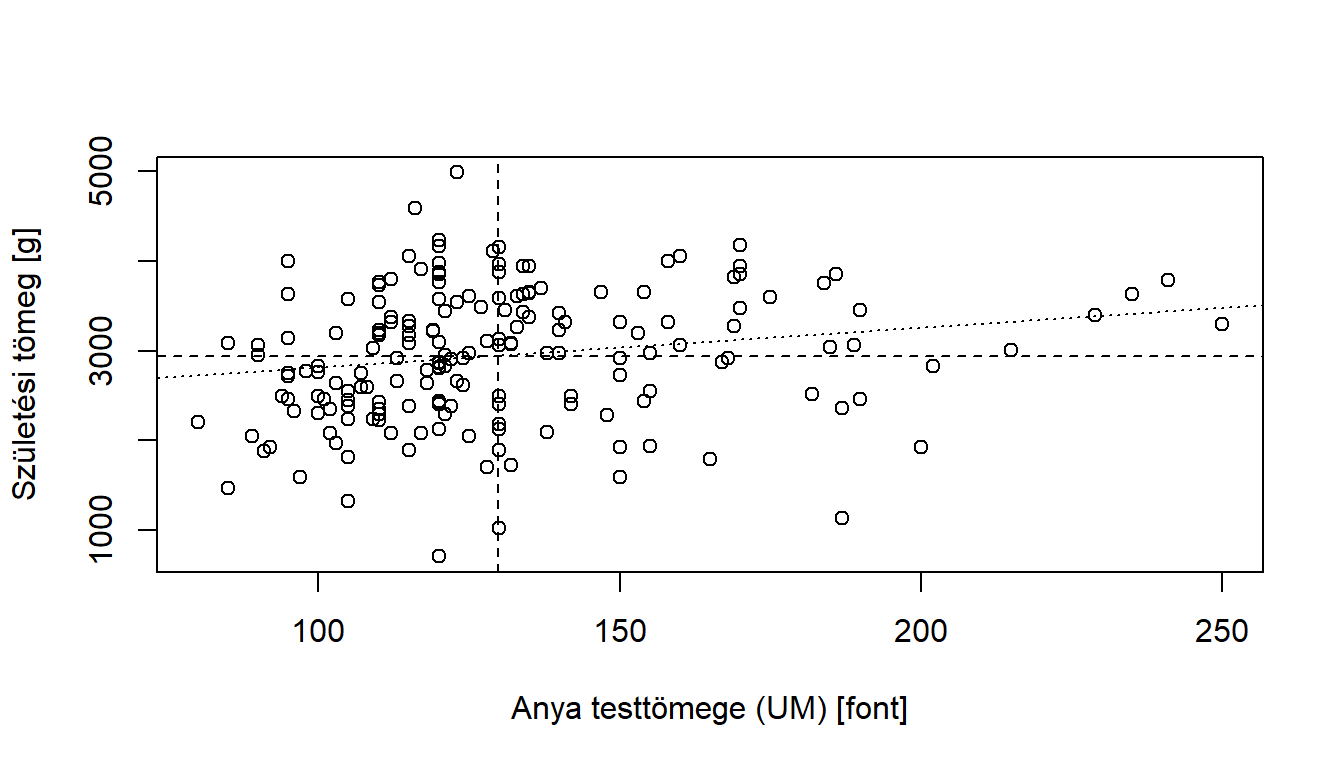
\includegraphics{bevbiostat_files/figure-latex/scatterplot-1.pdf}
\caption{\label{fig:scatterplot}Két mennyiségi változó kapcsolatának
ábrázolása szóródási diagrammal.}
\end{figure}

Az ábrán bejelöltük (szaggatott vonallal, a két tengellyel párhuzamosan)
a két változó átlagát is.

Jól látható, immár grafikusan is, hogy mit értünk a két változó közötti
kapcsolat fogalmán: a pontok tendenciájukban a szaggatott vonalak által
kijelölt koordináta-rendszer jobb felső és bal alsó kvadránsában
találhatóak (átlag feletti -- átlag feletti és átlag alatti -- átlag
alatti zónák). Természetesen látszik az is, hogy a kapcsolat
sztochasztikus, azaz van pont a több kvadránsban is (itt aztán pláne,
hiszen a kapcsolat nem is túl erős). Ne feledjük azt sem, hogy nem csak
a pontok darabszáma számít, hanem a konkrét helyzetük is (mennyire
,,erősíti meg'' a kapcsolat fennállását).

Ráerősítve az előbb mondottakra, az ábrán behúztuk a pontokra legjobban
illeszkedő egyenest is. Ahogy említettük, a kapcsolat ,,erőssége''
egyúttal azt is jelenti, hogy a pontok mennyire szorosan illeszkednek a
rájuk legjobban illeszkedő egyenesre (látható, hogy itt nem túl
szorosan).

Mindezeket szemlélteti a következő ábra is (\ref{fig:corrdemo}. ábra),
mely különböző korrelációs együtthatójú kapcsolatokat (különböző
előjelekkel és abszolút értékekkel, azaz különböző irányú és erősségű
kapcsolatokat) mutat be példákkal.

\begin{figure}
\centering
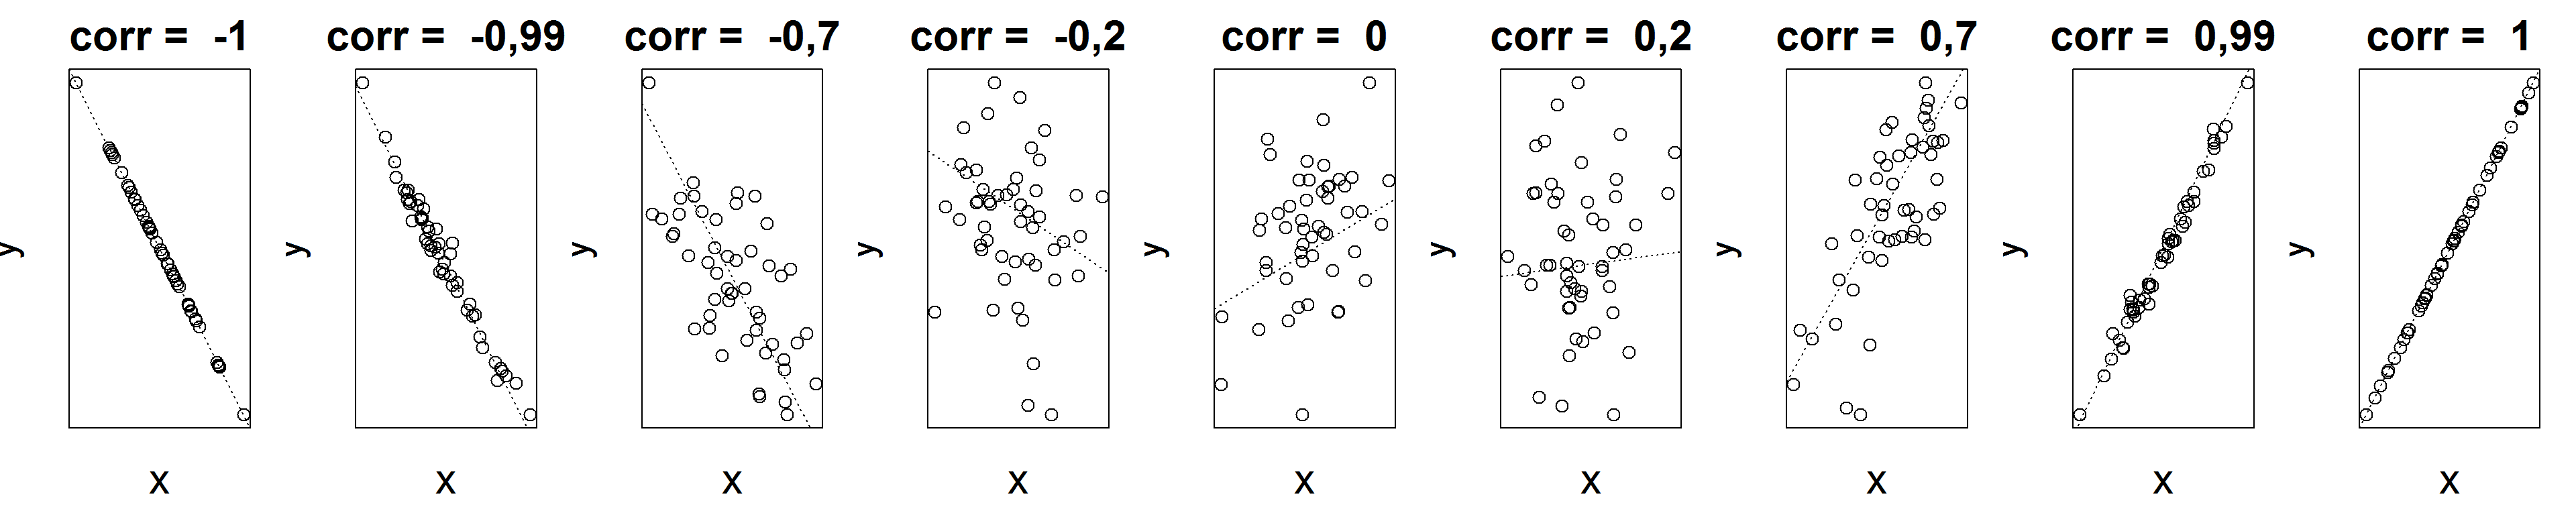
\includegraphics{bevbiostat_files/figure-latex/corrdemo-1.pdf}
\caption{\label{fig:corrdemo}Különféle korrelációs együtthatók
szemléltetése.}
\end{figure}

A grafikus ábrázolás előnye, hogy (szemben a korrelációs együtthatóval)
nem okoz gondot semmilyen outlier, nemlineáris kapcsolat stb. -- ezek
mind láthatóak lesznek az ábrán. (Itt is hangsúlyosan él tehát Tukey már
említett tanácsa\dots{}) Erre mutat példát a nevezetes Anscombe-kvartett
(\ref{fig:anscombe}. ábra). Az ábrák négy kétváltozós adatsor szóródási
diagramját mutatják. Mindegyiknek \emph{hajszálpontosan ugyanaz} a
korrelációs együtthatója (sőt, az átlaguk és a szórásuk is -- így
ugyanaz a rájuk legjobban illeszkedő egyenes is), mégis, a valós helyzet
drámaian más. Outlierek, nemlineáris kapcsolatok vannak jelen. Ez
azonban csak ábrázolás után derül ki, a korrelációs együttható
használata mindezt teljesen elfedné!

\begin{figure}
\centering
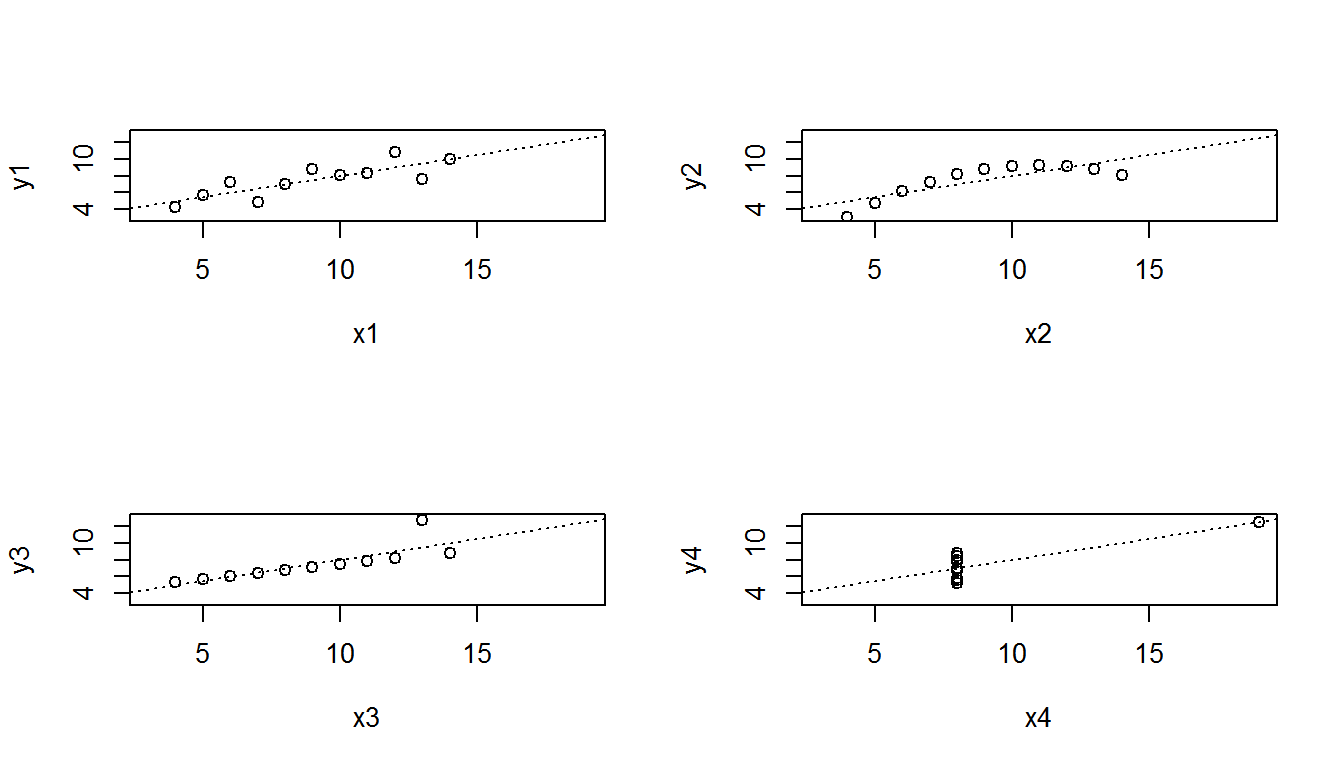
\includegraphics{bevbiostat_files/figure-latex/anscombe-1.pdf}
\caption{\label{fig:anscombe}Az Anscombe-kvartett.}
\end{figure}

Zárásként megjegyezzük, hogy ebben a grafikus ábrázolásban valóban
nincsen semmilyen információtömörítés. Az is igaz, hogy a kétváltozós
elemzés tartalmaz minden információt, amit a két egyváltozós elemzés: a
pontokat levetítve valamelyik tengelyre, visszakapjuk az adott tengely
változójának adatait; azokat csoportosítva (a tengelyt osztályközökre
bontva) rögtön készíthető például hisztogram. Szemléletesen látszik
azonban az is, hogy \emph{pusztán} a hisztogramokból (tehát az
egyváltozós adatokból) \emph{lehetetlen} lenne nyilatkozni a két változó
közti kapcsolatról. (Képzeljünk egy egy olyan esetet, melyben a változók
között erős kapcsolat van, de úgy, hogy mindkét változó önmagában
szimmetrikus. Ekkor nyugodtan tükrözhetnénk a szóródási diagramot
bármelyik átlagot jelentő szaggatott vonalra, az egyváltozós adatok
ugyanazok maradnának, noha kétváltozósan pont hogy megfordult a
kapcsolat iránya.) Ezért több a kétváltozós elemzés mint két egyváltozós
elemzés.

\section{További többváltozós
elemzések}\label{deskriptivtovabbitobbvalt}

A kétváltozós esetek tárgyalásából a fentiekben kimaradt az az eset,
amikor egy minőségi és egy mennyiségi változó kapcsolatát kell
vizsgálni. Ezt \emph{vegyes kapcsolatnak} szokás nevezni; részletesebben
most nem foglalkozunk vele.

A másik kérdés, ami felmerül, hogy mi a helyzet kettőnél több változó
esetén. Ha nem lényegesen több változóról van szó, akkor a fenti
módszerek -- több-kevesebb módosítással -- de kiterjeszthetőek. Például
a szóródási diagram elvileg három változós esetre változatlanul
kiterjeszthető (bár a gyakorlatban már ezt sem nagyon szokták használni,
hiszen egy három dimenziós pontfelhő csak számítógépen tekinthető meg
érdemben, és ott se túl áttekinthető emberi szemnek). Négy és annál több
dimenziónál már trükkre van szükség; a tipikus megoldás, hogy minden
lehetséges koordináta-párra levetítik a sokdimenziós pontfelhőt, és az
így kapott kétdimenziós szóródási diagramokat mutatják meg (mátrix
szóródási diagram). Egy-két tucat változó felett azonban már ez sem
igazán tekinthető át, illetőleg már nem nevezhető érdemben kettőnél több
dimenziós elemzésnek. Hasonló a helyzet a korrelációs együtthatóval,
illetve a kontingenciatáblával és elemzési eszközeivel.

\chapter{Induktív statisztika}\label{induktiv}

Ebben az alfejezetben röviden, az alapkoncepciókra fókuszálva bemutatjuk
a statisztika induktív ágát. Már volt róla szó, hogy az induktív
statisztika jellemzője, hogy \emph{tekintettel van} a mintavételi
helyzetre (azaz arra, hogy mi csak egy részét ismerjük azon sokaságnak,
melyre a kérdésünk irányult): azzal foglalkozik, hogy hogyan lehet
pusztán a mintában lévő információ alapján mégis a sokaságról
nyilatkozni. Innen a módszer neve: indukció a.m. következtetés,
tudniillik következtetés a mintából a sokaságra.

Elsőként röviden megismételjük, és pár fontos részlettel kibővítjük a
\textbf{mintavételi helyzettel} kapcsolatos ismereteinket; ezt követően
nagyon tömören, az alapelvekre szorítkozva bemutatjuk az induktív
statisztika két nagy területét: a becsléselméletet és a
hipotézisvizsgálatot. A \textbf{becsléselmélet} azzal foglalkozik, hogy
egy sokaságot jellemző paramétert, például a sokaság átlagát pusztán a
minta alapján ,,megtippeljünk'`(valamilyen szempontok szerint a lehető
legjobban). A \textbf{hipotézisvizsgálat} ennek bizonyos értelemben az
ikertestvére: célja, hogy a sokaság valamely jellemzőjére tett állítások
-- például a sokaság átlaga egy adott szám -- helyességét
,,megtippeljük'' pusztán a minta alapján.

\section{A mintavételi helyzet és
következményei}\label{induktivmintavetelihelyzet}

Ahogy már megbeszéltük, mintavételi helyzetről akkor beszélünk, ha a
\textbf{sokaságnak} (amire, definíció szerint, kutatási kérdésünk
vonatkozik), csak egy részét tudjuk megfigyelni. Ezt a megfigyelt részt
nevezzük \textbf{mintának}. Szintén volt róla szó, hogy a mintavételi
helyzet jelentősége a biostatisztikában hatalmas: nem csak azért, mert
egy sor gyakorlati esetben bár a sokaság elvileg teljeskörűen
megfigyelhető lenne, de erre gyakorlati okok (költség, időigény stb.)
miatt nincs mód, hanem azért is, mert biostatisztikában tipikusak az
olyan kérdések, melyek fiktív, végtelen sokaságra vonatkoznak (például:
,,Egy új vérnyomáscsökkentő gyógyszer-jelölt valóban csökkenti a
vérnyomást?''). Ilyen esetekben bármennyi megfigyelést is végzünk, az
szükségképp minta lesz.

Adódik tehát a feladat, hogy annak ellenére nyilatkozzunk a sokaságról,
hogy mi csak egy részét ismerjük. Nagyon sokan ezen a ponton
valószínűleg azt gondolják, hogy ez lehetetlen feladat -- valóban,
példának okáért, ha 1000 elemből csak 999-et ismerünk, akkor
\emph{elvileg} bármennyi lehet a sokaság (mind az 1000 elem) átlaga,
akármik is voltak a minta elemei.

Az a megállapítás azonban, hogy ,,semmit nem tudunk mondani'' a
sokaságról, szerencsére túlzás. A helyes megfogalmazás az, hogy
\emph{biztosat} nem tudunk mondani a sokaságról\dots{} de valószínűségi
kijelentéseket továbbra is tudunk tenni! Ha ugyanis megfelelően történt
a mintavétel (erre még visszatérünk), akkor már a minta is elárult
valamit a sokaságról, tudni fogunk valamit azokról a valószínűségi
törvényszerűségekről, melyek az ismeretlen elemek viselkedését (is)
áthatják. Ez pedig lehetővé fogja tenni, hogy ugyan csak sztochasztikus
értelemben, de azokról is nyilatkozzunk.

Az tehát nem igaz, hogy semmit nem tudunk mondani a sokaságról, de azzal
valóban együtt kell élnünk, hogy az induktív statisztikában -- szemben a
deskriptívvel -- már csak \emph{bizonytalansággal terhelt} állításokat
tudunk tenni. Szerencsére azonban arra is képesek leszünk, hogy e
bizonytalanság mértékét magát is becsüljük (persze ismét csak:
bizonytalansággal terhelten).

Nyilvánvaló, hogy bármilyen induktív statisztikai feladatot is kell
megoldanunk, ahhoz csak a mintában lévő információt tudjuk felhasználni
(ez épp a minta definíciója). Márpedig ha csak a sokaság egy részét (a
mintát) ismerjük, akkor \emph{bármilyen}, mintából számolt jellemző két
dologtól fog függeni:

\begin{enumerate}
\def\labelenumi{\arabic{enumi}.}
\tightlist
\item
  a jellemző sokaságbeli értékétől,
\item
  attól, hogy konkrétan hogy választottuk ki a mintát.
\end{enumerate}

Példának okáért, egy minta átlagát két dolog fogja befolyásolni: a
sokaság átlaga (ha ez nagyobb, akkor várhatóan egy minta átlaga is
nagyobb lesz) és az, hogy konkrétan melyik elemeket választottuk ki a
sokaságból (adott sokasági átlag mellett is választhatunk -- tökéletesen
véletlen mintavétel mellett is! -- pont kisebb, és pont nagyobb elemeket
is).

Mi értelemszerűen csak az elsőre vagyunk kíváncsiak, de sajnos a második
hatása elvileg is kiküszöbölhetetlen. Bármilyen módszert is találunk ki
arra, hogy a mintából hogyan következtessünk a sokaságra, teljesen
biztos, hogy annak a végeredménye \emph{mintáról-mintára változni} fog,
azaz függeni fog attól, hogy konkrétan ,,hogyan nyúltunk bele a
sokaságba'', konkrétan milyen mintát vettünk. Ezt a jelenséget hívjuk
\textbf{mintavételi ingadozásnak}. A szerencse épp az lesz, hogy ez a
mintavételi ingadozás követni fog bizonyos (valószínűségi)
törvényszerűségeket, így bár a fenti miatt elkerülhetetlenül hibázhatunk
a következtetésnél, de annak természetéről fogunk tudni nyilatkozni.

Amit nagyon fontos megérteni, hogy az előbb említett ,,hibázás'' alatt
nem arra kell gondolni, hogy valamilyen értelemben rosszul vesszük a
mintát. Ha egy 1000 fős sokaságból veszünk egy 30 fős mintát a sokasági
átlag becslésére, akkor előfordulhat, mégpedig a \emph{legtökéletesebben
véletlen} mintavétel mellett is, hogy épp a 30 legkönnyebb embert
választjuk ki a sokaságból. Természetesen, ha rosszul veszünk mintát
(például akár tudattalan módon is, de a soványabb embereket szólítjuk
meg a kérdőívvel, hogy ne hozzuk zavarba a megkérdezetteket), akkor
elképzelhető, hogy ennek megnő a valószínűsége, de akkor sem nulla ha
tökéletesen véletlen a mintavétel.

Csak épp -- és itt jön a lényeg -- extrém kicsi! Ha tényleg tökéletesen
véletlen a mintavétel, azaz minden sokasági alanynak azonos esélye van a
mintába kerülésre, akkor annak a valószínűsége, hogy pont a 30
legsoványabbat választjuk ki épp
\(1/\binom{30}{1000}\approx 4\cdot 10^{-56}\)\%. Így értendő az, hogy a
hiba valószínűségszámítási úton, ,,sztochasztikusan'' limitálható: nem
tudjuk kizárni, hogy ilyen -- hatalmas méretű -- torzítás keletkezzen a
mintából következtetés hatására\dots{} de meg tudjuk mondani, hogy ennek
mennyi a -- szerencsére igen kicsi -- valószínűsége. Az ilyen okokból
fakadó hibázást nevezzük \textbf{mintavételi hibának}.

Nem csak olyan hiba van azonban, ami az -- elkerülhetetlen --
mintavételi ingadozásból adódik. Véthetünk hibát alullefedéssel és
túllefedéssel (azaz a minta pontatlan körülírásával), véthetünk
definíciós hibát a kérdéseknél, hibát az adatkódolás során, a végpont
megválasztásánál stb. stb., de ami még fontosabb, hogy véthetünk hibát a
minta kijelölésével (amennyiben a minta valójában nem reprezentatív a
sokaságra nézve, lásd az előbbi példát a személyes megkérdezéses
testtömeg-vizsgálatról), vagy épp megfigyeléses vizsgálat esetén a
confounding-gal. Ezeket -- tisztán statisztikai úton nem olyan könnyen
kézben tartható -- hibákat nevezzük egységesen \textbf{nem-mintavételi
hibáknak}.

\section{Becsléselmélet}\label{induktivbecsleselmelet}

A becsléselmélet az induktív statisztika egyik fő ága, feladata
valamilyen sokasági jellemző értékének minta alapján történő
megbecslése. A ,,becslés'' szó használata azért indokolt, mert az előbb
kifejtettekből világos, hogy mintavételi helyzetben csak valószínűségi
jellegű kijelentések tételére van mód.

A sokasági jellemzőt teljesen
általánosan\footnote{Ebbe természetesen beletartozhat több jellemző egyszerre történő becslése is, mi most azonban az ún. egydimenziós paraméterbecslésekre fogjuk korlátozni magunkat.}
értjük (ha nem specifikáljuk közelebbről, akkor általában \(\theta\)-val
jelöljük), bármilyen, a sokaság ismeretében számszerűen meghatározható
értéket jelenthet (például a sokaság átlagát, szórását, valamilyen
tulajdonsággal rendelkező elemeinek az arányát stb.). Egy tipikus példa
a sokaság átlagának/várható értékének
becslése\footnote{Átlagról általában akkor beszélünk, amikor a sokaság véges, ilyenkor tipikusan úgy képzeljük (,,elemeivel adott sokaság''), hogy a sokaságot véges sok érték felsorolásával megadhatjuk; várható értéket általában akkor mondjuk, ha a sokaság fiktív, végtelen, ilyen tipikusan úgy gondoljuk (,,eloszlásával adott sokaság''), hogy azt a háttéreloszlást ismerjük, melyet a sokaság minden egyes eleme követ, legegyszerűbb esetben független és azonos eloszlású módon.}.
Egy teljesen természetes gondolat, hogy ezt a jellemzőt a minta
átlagával igyekezzünk megbecsülni.

Ez a naiv ,,tipp'' is mutatja már, hogy mit értünk precízen becslés
alatt: egy olyan függvényt (neve \textbf{becslőfüggvényt} vagy
egyszerűen \textbf{becslő}), melynek bemenetül a minta elemeit kell
megadni, eredményként pedig kidobja a becslést az ismeretlen sokasági
jellemzőre. Egy \(\theta\) sokasági jellemző becslőfüggvénye tehát egy
\[
    \widehat{\theta} = f\left(x_1,x_2,\ldots,x_n\right)
\] függvény. (A becsült értéket a statisztikában általában is kalappal
jelöljük.) Az előbbi naiv példánk azt jelenti, hogy ha a becsülni kívánt
jellemző a sokasági várható érték (\(\theta=\mu\)), akkor reményeink
szerint arra jó becslő lesz az \[
    f\left(x_1,x_2,\ldots,x_n\right)=\frac{\sum_{i=1}^n x_i}{n}=\overline{x}
\] függvény. Ahogy már korábban is megállapítottuk, ennek értéke két
dologtól fog függeni: a \(\mu\) értékétől (a valódi sokasági
jellemzőtől), és attól, hogy konkrétan milyen mintát vettünk. Ez utóbbi
hatás miatt természetesen a becslőfüggvény eredménye minden egyes mintán
más és más lesz.

Felmerül a kérdés, hogy mit értünk precízen ,,jó'' becslőfüggvény alatt.
A gyakorlatban két tulajdonság különösen fontos: 1. Elfogadjuk, hogy a
becslőfüggvény által szolgáltatott becslés mintáról-mintára ingadozik,
de legalább az teljesüljön, hogy az ingadozás centrumában a valódi
(sokasági) jellemző legyen, olyan értelemben, hogy \emph{átlagosan} jó
legyen a becsült érté. E tulajdonság neve: \textbf{torzítatlanság}. 2.
Ennek az ingadozásnak a mértéke lehetőleg minél kisebb legyen, e
tulajdonság neve: \textbf{hatásosság}.

Amint említettük is, a becslőfüggvény értéke (tehát az adott mintából
számolt becslés) nem állandó, hanem mintáról-mintára ingadozik.
Visszatérve az egyszerű példánkra az 1000 elemű, véges sokaságból
történő átlagbecslésre: kaphatjuk, mintavételtől függően, a legkönnyebb
30 ember átlagát is becslésként, és a legnehezebb 30 átlagát is. (És
természetesen egy sor értéket a kettő között.) De, amint már ott is
megállapítottuk, ezen extrémumok valószínűsége kisebb, a közbülső (és
ilyen módon a valósághoz közelebb álló) értékeké pedig -- szerencsére --
nagyobb. Más szóval arra jutottunk, hogy a becslőfüggvény értékeinek is
van egy eloszlása: meg lehet adni, hogy adott tartományba eső becslést
mekkora valószínűséggel adnak. Ezt nevezzük \textbf{mintavételi
eloszlásnak}.

Ennek ismeretében már teljesen pontosan is definiálhatjuk a fenti
tulajdonságokat: egy becslőfüggvényt torzítatlannak mondunk, ha a
mintavételi eloszlásának a várható értéke a valódi (sokasági) jellemző,
a hatásosságot pedig a mintavételi eloszlás szórásával mérhetjük. (Egy
becslőfüggvényt hatásosnak mondunk, ha torzítatlan, és a torzítatlan
becslők körében minimális szórású.)

Azzal a kérdéssel, hogy hogyan lehet egy becslőfüggvényt ,,kitalálni''
(tehát, ha megadnak egy paramétert, akkor mutatni egy rá vonatkozó, és
persze lehetőleg minél jobb statisztikai tulajdonságokkal bíró
becslőfüggvényt) nem foglalkozunk részletesebben, csak megemlítjük, hogy
erre vonatkozóan jól bejáratott módszerek, ún. becslési elvek léteznek.
(A legnevezetesebb közülük a maximum likelihood-elv, továbbá a plug-in
becslés, a legkisebb négyzetek elve, a momentumok módszere és a
Bayes-becslés.)

Nézzünk minderre egy példát! Tekintsünk egy (eloszlásával adott)
sokaságot, mely \(X\sim\mathcal{N}\left(\mu,\sigma_0^2\right)\)
eloszlást követ. (Tehát tetszőleges számú mintát vehetünk belőle; minden
egyes ilyen mintaelem egy ilyen eloszlásból származó, egymástól
független szám lesz.) Azt állítjuk (és ezt hamarosan szabatosabban is be
fogjuk bizonyítani), hogy ekkor a belőle vett \(n\) elemű minták átlaga,
azaz a \(\mu\) sokasági várható érték (mint sokasági jellemző) fenti
becslőfüggvénye
\(\overline{x}\sim\mathcal{N}\left(\mu,\sigma_0^2/n\right)\) eloszlást
fog követni. (Tehát most feltételeztük, hogy azt \emph{a priori} tudjuk,
hogy normális eloszlású a sokaság, sőt, \(\sigma_0\)-t is ismertnek
vesszük, azaz csak a \(\mu\) a kérdés.) Jegyezzük meg, hogy a sokasági
jellemző, amit becsülni szeretnénk, itt a \(\mu\) maga; az tehát nem
követ semmilyen eloszlást, egy -- konstans -- szám! (Csak mi nem
ismerjük.) A következőkben ezt az állítást fogjuk matematikai úton,
valószínűségszámítási eszközökkel bebizonyítani, mégpedig a
legegyszerűbb esetre, a fent vázolt független és azonos eloszlású
mintavételre.

Legyen az \(n\) elemű mintánk
\(X_1,X_2,\ldots,X_n\sim\mathcal{N}\left(\mu,\sigma_0^2\right)\)
függetlenül (mivel a mintavétel azonos eloszlású is, így mindegyik
ugyanolyan eloszlást követ, ezért volt azt elég egyszer leírni).
Figyeljük meg, hogy itt nagy betűket írtunk: ezek nem konkrét
(realizálódott) értékek, hanem maguk is valószínűségi változók. (Most
ugyanis statisztikai analízisét adjuk a helyzetnek: úgy képzeljük, hogy
még nem vettünk mintát, hanem épp ellenkezőleg, azt vizsgáljuk, hogy
,,mi minden történhet'' amikor majd mintát veszünk.) Ezzel a
becslőfüggvényünk: \[
    \overline{X}=\frac{\sum_{i=1}^n X_i}{n}.
\]

Valószínűségszámításból tudjuk, hogy 1. Normális eloszlású valószínűségi
változók összege normális (szépen megfogalmazva: a normális
eloszláscsalád zárt a konvolúcióra). 2. A várható érték lineáris, így
egy összeg várható értéke a várható értékek összege. 3. Ha ráadásul
korrelálatlan (de csak ez esetben!), akkor a szórásnégyzetek -- nem a
szórások! -- is összeadódnak. Ebből a háromból már következik, hogy \[
    \sum_{i=1}^n X_i\sim\mathcal{N}\left(n\mu,n\sigma_0^2\right).
\] Szintén valószínűségszámításból tudjuk, hogy
\(\mathbb{E}\left(aX\right)=a \cdot \mathbb{E}X\) és
\(\mathbb{D}^2\left(aX\right)=a^2 \cdot \mathbb{D}^2 X\), ezekből pedig
már következik, hogy \[
    \overline{X}=\frac{\sum_{i=1}^n X_i}{n} \sim \mathcal{N}\left(\mu,\sigma_0^2/n\right),
\] ahogy azt eredetileg állítottuk is.

Ezzel igazoltuk, hogy ilyen körülmények mellett a mintaátlag torzítatlan
becslője a sokasági átlagnak, sőt, kiszámoltuk a mintavételi szórását
is. (Be lehetne látni kicsit komolyabb matematikai statisztikai
eszközökkel, hogy ez ráadásul e körülmények között hatásos becslő is,
tehát ennél kisebb mintavételi szórás el sem érhető a torzítatlan
becslők körében.)

Ez tehát azt jelenti, hogy a 2944,6 gramm nem csak a születési tömegek
átlaga (ahogy azt az előbb mondtuk), hanem egyúttal a ,,vizsgálat
beválogatási feltételeinek megfelelő újszülöttek'' (fiktív, végtelen!)
sokaságának várható értékének becslője is! Nem csak azt mondhatjuk, hogy
2944,6 gramm a mintaátlag (biztosan), hanem azt is, hogy ez a legjobb
tippünk arra, hogy mennyi a sokaság várható értéke. Vegyük észre, hogy
minket valójában ez utóbbi érdekel! Tehát bár a számérték itt pont
ugyanaz lett (ez nincs mindig így!), az igazán érdekes eredmény az
utóbbi megfogalmazás (hiszen minket nem \emph{konkrétan} ez a 189
újszülött érdekel, hanem \emph{általában} az ilyen újszülöttek
jellemzőinek viselkedése).

Mind ez idáig azonban csak olyan becslőfüggvényekről beszéltünk, melyek
egyetlen értéket, ,,a'' legjobb becslést adják vissza eredményként. Az
ilyen becslést hívjuk \textbf{pontbecslésnek}. (Hiszen az eredménye
egyetlen pont a számegyenesen.) Ez olyan szempontból azonban nem
szerencsés, hogy az eredmény semmit nem mond az abban lévő
bizonytalanságról -- noha, legalábbis becsülni, azt is tudnánk!

Azt a becslési módszert, ami ezen túllép és explicite megjeleníti a
becslésben lévő bizonytalanságot is, \textbf{intervallumbecslésnek}
nevezzük. Az intervallumbecslés központi eszköze az
\textbf{konfidenciaintervallum} (CI): ez egy olyan intervallum, melyre
igaz, hogy a hogy ha sokszor megismételnék a mintavételt, és mindegyik
mintából megszerkesztenénk a CI-t, akkor ezen CI-k várhatóan adott, nagy
hányada (például 95\%-a) tartalmazná az igazi (sokasági) értéket. Ez
esetben ezt az intervallumot 95\% megbízhatóság melletti
konfidenciaintervallumnak nevezzük. A 95\%, mint paraméter neve
\textbf{megbízhatósági szint}, általában \(1-\alpha\)-nak nevezzük
(tehát \(\alpha=0,\!05\) mellett beszélünk 95\%-os megbízhatóságról).
Első ránézésre kicsit furcsa lehet ez a jelölés, de majd a
hipotézisvizsgálatnál is látni fogjuk, hogy \(\alpha\)-val valamilyen
hibázás jellegű mennyiséget szeretnénk jelölni, nem jóságot.

Az induktív statisztikában tehát elfogadjuk (kénytelenek vagyunk
elfogadni), hogy a becslésünk eredménye mintáról mintára változik, és
így nem tudhatjuk biztosan, hogy \emph{adott mintából} számolt becslés
hogyan viszonyul a valódi (sokasági) értékhez -- a
konfidenciaintervallum azonban épp azt próbálja megragadni, hogy --
adott minta alapján! -- mire tippelhetünk, ,,vélhetően'`hol lehet a
valódi sokasági érték (adott, nagy megbízhatósággal). Ez természetesen
már nem egyetlen szám, hanem egy tól-ig intervallum lesz a jellemzőre
vonatkozóan. Hogy mit jelent a ,,vélhetően'`és a ,,megbízhatóság'', az
pontosításra szorul, erre tárgyalásunk legvégén fogunk visszatérni.

Adott megbízhatósági szint mellett minél szűkebb a CI, annál kisebb a
bizonytalanság a becslésünkben. Természetesen adott becslés mellett a CI
szélességét a megbízhatósági szint fogja meghatározni: kis megbízhatóság
mellett szűk intervallumot is mondhatunk, de ha nagy megbízhatóságra van
szükségünk, akkor csak széles limiteket tudunk szabni. Itt tehát
kompromisszumot kell kötnünk: az se jó, ha nagy biztonsággal tudjuk,
hogy nem igazán tudjuk, hogy hol van az igazi érték, és az se, ha nagyon
kis biztonsággal tudjuk, hogy igen pontosan hol van\dots{} A 95\% egy
tipikus, gyakorlatban igen sokszor használt kompromisszum ez ügyben.

Nézzünk erre is egy számszerű példát! Folytatva előző példánkat, tudjuk,
hogy \(\overline{X} \sim \mathcal{N}\left(\mu,\sigma_0^2/n\right)\).
Ebből következik, hogy \[
    \frac{\overline{X}-\mu}{\sigma_0/\sqrt{n}}\sim\mathcal{N}\left(0,1\right),
\] azaz \[
    \mathbb{P}\left(-z<\frac{\overline{X}-\mu}{\sigma_0/\sqrt{n}}<z\right)=\Phi\left(z\right)-\Phi\left(-z\right)=\Phi\left(z\right)-\left[1-\Phi\left(z\right)\right]=2\Phi\left(z\right)-1.
\] Ha ezt a valószínűséget \(\left(1-\alpha\right)\)-nak választjuk (a
megbízhatósági szint fenti értelme miatt), akkor kapjuk, hogy
\(\Phi\left(z\right)=1-\frac{\alpha}{2}\) azaz
\(z=\Phi^{-1}\left(1-\frac{\alpha}{2}\right)\). Erre a mennyiségre
bevezetve a \(z_{1-\frac{\alpha}{2}}\) jelölést, rögtön látható, hogy a
\(\left[\mu-z_{1-\frac{\alpha}{2}}\frac{\sigma_0}{\sqrt{n}},\mu+z_{1-\frac{\alpha}{2}}\frac{\sigma_0}{\sqrt{n}}\right]\)
tartományba \(1-\alpha\) valószínűséggel esik \(\overline{X}\). Ezt
nevezhetnénk ,,deduktív statisztikának'', hiszen itt a sokaságot
tekintettük ismertnek, és ez alapján következtettünk a minta
viselkedésére.

Átrendezve ,,kapjuk'' a minket érdeklő az induktív statisztikát: \[
    \mathbb{P}\left(-z_{1-\frac{\alpha}{2}}<\frac{\overline{X}-\mu}{\sigma_0/\sqrt{n}}<z_{1-\frac{\alpha}{2}}\right)=1-\alpha \Rightarrow \mathbb{P}\left(\overline{X}-z_{1-\frac{\alpha}{2}}\frac{\sigma_0}{\sqrt{n}}<\mu<\overline{X}+z_{1-\frac{\alpha}{2}}\frac{\sigma_0}{\sqrt{n}}\right)=1-\alpha.
\] Ekkor a konfidenciaintervallum immár egy konkrét mintára a fenti
alapján: \[
    \left[\overline{x}-z_{1-\frac{\alpha}{2}}\frac{\sigma_0}{\sqrt{n}},\overline{x}+z_{1-\frac{\alpha}{2}}\frac{\sigma_0}{\sqrt{n}}\right].
\] Tipikusan \(\alpha=0,\!05\), amint mondtuk, ekkor
\(1-\alpha=95\)\%-os konfidenciaintervallumról beszélünk.

\emph{Nagyon fontos} megfigyelni, hogy csak mintavétel \emph{előtt}
vannak valószínűségi változók (,,nagy betűk'`), \emph{utána} már nem
(,,kis betűk'`) -- ezért használtuk a megbízhatóság szót a valószínűség
helyett. Mintavétel \emph{után} ugyanis már nem tehetünk olyan
kijelentést, hogy a megkonstruált CI 95\%-os
,,valószínűséggel'`tartalmazza a valódi, sokasági paramétert, hiszen ha
már egy realizálódott minta van a kezünkben, akkor elvileg akárhol lehet
a valódi érték, erről semmi közelebbit nem tudunk mondani.
Valószínűséget csak a (szükségképp képzeletbeli) ,,ismételt
mintavételi'`értelemben tudunk behozni a feladatba, ezért használjuk
megkülönböztetésül a megbízhatóság szót. Így kell érteni, hogy a
konfidenciaintervallum jellemzi, hogy ,,hol lehet'' a valódi (sokasági)
paraméter.

A születési tömegek 95\%-os konfidenciaintervalluma {[}2840,0--3049,2{]}
gramm. (Megjegyezzük, hogy ez a fentitől kissé eltérő módszerrel
készült, ami tekintettel van arra is, hogy itt most -- szemben a fenti
példával -- nem ismerjük \emph{a priori} a sokaság szórását.) Ez azt
jelenti, hogy a \emph{legjobb} tippünk a születési tömeg sokasági
várható értékére a 2944,6 gramm, de azt is tudjuk ezen felül mondani,
hogy bár ez csak bizonytalan tipp (hiszen a becsült érték
mintáról-mintára ingadozik), de 95\%-os \emph{megbízhatósággal} azért
kijelenthető, hogy nem kisebb a keresett, ismeretlen sokasági várható
érték mint 2840,0 gramm és nem nagyobb mint 3049,2 gramm. (Amit úgy
értünk, hogy azt becsüljük, hogy ha a sokaságból 100 mintát vennénk, és
mindegyikből ugyanígy megkonstruálnánk a konfidenciaintervallumokat,
akkor várhatóan 95 esetben tartalmazná a CI a valódi, sokasági értéket.)
Érdemes megfigyelni, hogy a konfidenciaintervallum két végpontja
szimmetrikus a pontbecslésre; ez a várható érték becslésére jellemző, de
más paramétereknél nem feltétlenül van így.

\section{Hipotézisvizsgálat}\label{induktivhipotezisvizsgalat}

Az induktív statisztika másik nagy ága a hipotézisvizsgálat. A
hipotézisvizsgálat nagyon sok szempontból a becsléselmélet, ezen belül
is az intervallumbecslés elméletének ikertestvére (ami ekvivalens, csak
átfogalmazottan felírt egyenletekre vezet), mégis, saját szóhasználata,
fogalomköre, és hatalmas gyakorlati jelentősége indokolja, hogy külön
tárgyaljuk.

Amíg a becsléselmélettől azt vártuk, hogy nyilatkozzon egy számunkra
ismeretlen jellemzőről, addig a hipotézisvizsgálat esetében van előzetes
elképzelésünk a jellemző értékéről (például, hogy egy adott számmal
egyenlő) -- csak épp nem tudjuk, hogy ez igaz-e. Ha az előzetes
feltevésünk mintára vonatkozna, akkor nem is volna semmi probléma:
kiszámítjuk a jellemzőt a mintából, és megnézzük, hogy teljesült-e a
feltevésünk. Mivel azonban a feltevés a sokaságra vonatkozik, így megint
csak visszatérünk oda, hogy erről biztos döntést hozni lehetetlen minta
alapján -- de valószínűségit lehet. Nem tudjuk megmondani, hogy a
sokaság átlagos testtömege 70 kg-e, ha a mintabeli átlag 65 kg\dots{} de
meg fogjuk tudni mondani (egyéb mintaadatok felhasználásával), hogy
\emph{mennyire hihető}, hogy 70 kg a sokasági átlag. Erre szolgál a
hipotézisvizsgálat. Már most fontos megjegyezni, hog a
hipotézisvizsgálat logikája bizonyos szempontból fordított: az előbbi
kérdés ellentétére keresi a választ, arra, hogy ha 70 kg \emph{lenne} a
sokasági átlag, akkor mennyire lenne valószínű, hogy ettől olyannyira
eltérő eredményt kapunk, mint a 65 (vagy annál is kisebb). Ha nagyon,
akkor azt mondjuk, hogy ,,minden bizonnyal'' nem 70 kg volt az átlag.

A problémát nyilván az adja, hogy -- maradva a fenti példánál -- nem
tudhatjuk, hogy mi okozta ezt az 5 kg különbséget. Valójában tényleg 70
kg a sokaság átlaga, csak a mintavételi ingadozás játéka miatt pont
olyan mintát fogtunk ki, amiben picit kisebb volt az átlag, vagy ez az 5
kg különbség olyan nagy, ami túlmutat a mintavételi ingadozáson, és azt
kell feltételeznünk, hogy a hátterében sokasági hatás (is) van (tehát,
hogy a sokasági átlag kisebb mint 70 kg)\dots{}?

Amint a fentiekből is kiderült, a hipotézisvizsgálat mindig a sokaságra
megfogalmazott állításból indul ki. Valójában nem is egy, hanem rögtön
két állítást használ a hipotézisvizsgálat; nevük nullhipotézis (\(H_0\))
és ellenhipotézis (\(H_1\)) melyek jellemzően egymás komplementerei.
(Azaz egymást kizárják, de a kettőből valamelyik biztosan fennáll.) A
fenti példát így írhatnánk:

\begin{align*}
    H_0&: \mu = \mu_0\\
    H_1&: \mu \neq \mu_0\\
\end{align*}

úgy, hogy \(\mu_0\)=70 kg.

Amit fontos észben tartani, hogy hipotézisvizsgálatnál az erős döntés
mindig az elutasítás tud lenni, ezért a legtöbb próba úgy van
megszerkesztve, hogy a szakmailag ,,izgalmas'`állítás, a tudományos
nóvum (hatásos a gyógyszer, van eltérés a laboreredményben stb.) az
ellenhipotézisbe kerüljön. Pontosan emiatt az elutasítás esetén nagyon
gyakran -- szinonimaként -- azt mondjuk, hogy a ,,próba szignifikáns''.

A hipotézisvizsgálat központi eszköze a \textbf{próbafüggvény} (vagy más
szóval \textbf{tesztstatisztika}). Az egész eszközt együtt
\textbf{tesztnek} vagy \textbf{próbának} nevezzük. A próbafüggvény a
mintaelemek függvénye, ilyen módon a próbafüggvénynek is eloszlása lesz.
És itt jön a kulcs: a próbafüggvényt úgy választjuk meg, hogy \(H_0\)
fennállása esetén valamilyen \emph{pontosan ismert} eloszlást kövessen;
ezt szokás \emph{nulleloszlásnak} is nevezni. Természetesen a
próbafüggvény \emph{konkrét értéke} függeni fog a mintaelemektől, de az
\emph{eloszlása} nem függhet ettől (sem más, ismeretlen paramétertől, ha
volna ilyen).

Hogy megértsük, hogy ez miért lesz alkalmas a hipotézispárról történő
(valószínűségi) döntéshozatalra, nézzünk egy konkrét példát. Folytatva
az előző példát, tegyük fel, hogy sokaságunk eloszlása normális, ismert
szórással. Amint már megbeszéltük, ekkor
\(\overline{X}= \sim \mathcal{N}\left(\mu,\sigma_0^2/n\right)\). Ez
tehát a mintaelemek függvénye, és elvileg próbafüggvénynek is nevezhető,
mert ha érvényesítjük rajta \(H_0\)-t (azaz \(H_0\)-t igaznak fogadjuk
el), akkor azt kapjuk, hogy
\(\overline{X}= \sim \mathcal{N}\left(\mu_0,\sigma_0^2/n\right)\), ami
valóban már nem függ ismeretlen paramétertől. Ezzel, és a technikailag
szintén megfelelő
\(\overline{X}-\mu_0\sim \mathcal{N}\left(0,\sigma_0^2/n\right)\)-nel is
az a gyakorlati baj azonban, hogy nagyon nehézkes lenne a használatuk,
hiszen bár a nulleloszlás ismert, de minden \(\mu_0\)-ra,
\(\sigma_0\)-ra és \(n\)-re más és más -- azaz ezektől függően minden
egyes hipotézisvizsgálathoz elő kéne keresni az adott eloszlást.

A \(\overline{X}-\mu_0\) azonban már mutatja az utat: próbálkozzunk a
\(\frac{\overline{X}-\mu_0}{\sigma/\sqrt{n}}\) próbafüggvénnyel (jele
általában \(Z\))! Ez már minden szempontból tökéletes lesz, hiszen
nulleloszlása \(\mathcal{N}\left(0,1\right)\), azaz minden paramétertől
függetlenül ugyanaz; egyetlen eloszlással elvégezhető az összes ilyen
típusú hipotézisvizsgálat e körülmények között.

Foglaljuk össze hol tartunk! Konstruáltunk egy olyan függvényét a
mintaelemeknek, melynek ismerjük az eloszlását \emph{ha} fennáll a
nullhipotézis. Ki tudjuk azt is számolni, hogy mennyi ennek a
próbafüggvénynek az értéke a konkrét (realizálódott) mintánkból; ezt
szokás empirikus értéknek (\(z_{\mathrm{emp}}\)) is nevezni. Innentől
úgy okoskodhatunk: biztos döntést lehetetlen hozni (ez az előbbi példán
nagyon jól látszik: a \(\mathcal{N}\left(0,1\right)\) nulleloszlás
tartója az egész számegyenes, tehát még ha fenn is áll a nullhipotézis,
elvileg \emph{akármilyen} szám realizálódhat belőle, az elvileg
bármilyen szám lehet a mintából kiszámított próbafüggvény értéke, azaz
\(z_{\mathrm{emp}}\)), de mégis, mennyire hihető, hogy a szaggatott
vonallal jelölt érték a folytonosan behúzott eloszlásból realizálódott a
következő esetekben (\ref{fig:hipalap}. ábra).

\begin{figure}
\centering
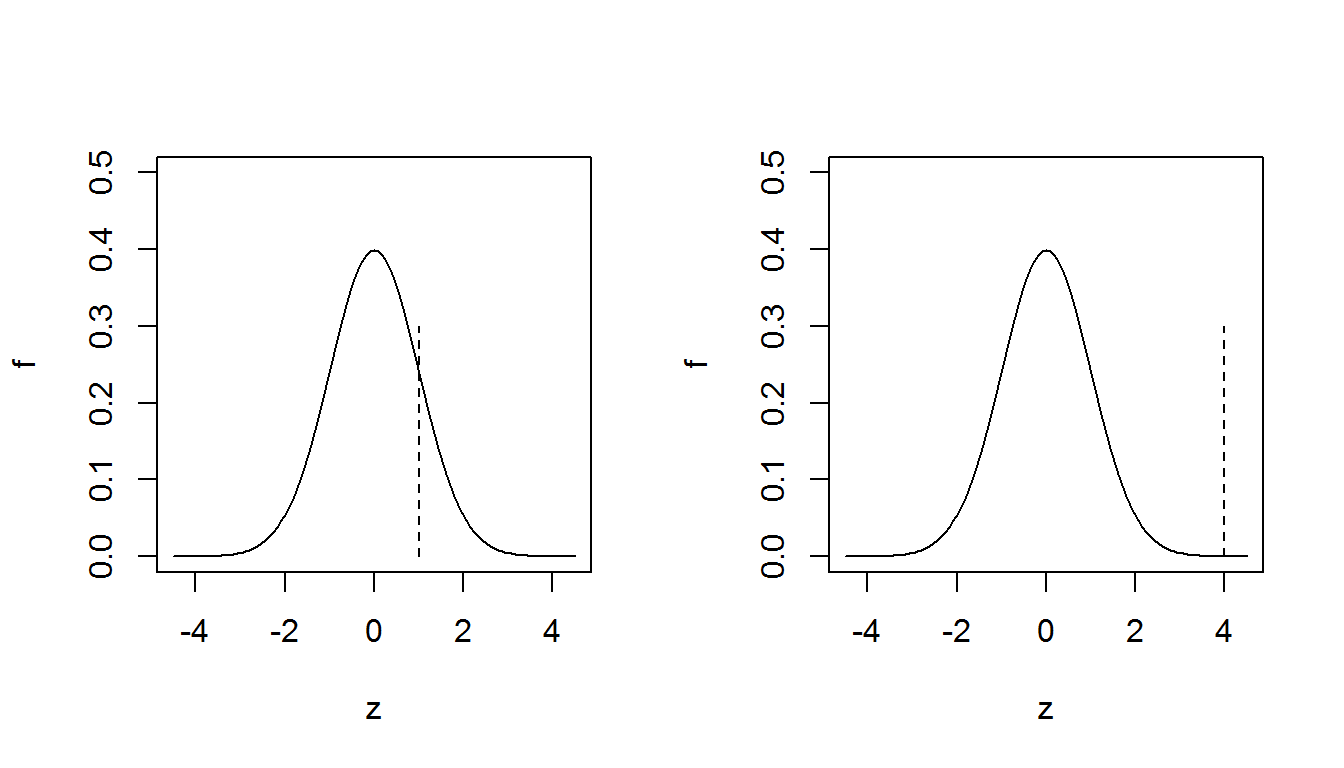
\includegraphics{bevbiostat_files/figure-latex/hipalap-1.pdf}
\caption{\label{fig:hipalap}A hipotézisvizsgálat alapgondolatának
szemléltetése.}
\end{figure}

Érezhető, hogy bár \emph{elvileg} mindkettő előfordulhat, de a bal
oldalit \emph{hajlamosak vagyunk} elhinni, a jobb oldalinál viszont épp
ellenkezőleg, \emph{hajlunk arra}, hogy azt gondoljuk, hogy az empirikus
érték valójában más eloszlásból realizálódott. Noha elvileg a bal oldali
is jöhet más eloszlásból, és a jobb oldali is ebből -- ezért a
bizonytalan megfogalmazások, mutatva, hogy ezek csak valószínűségi
állítások.

Precízebben megfogalmazva: az kicsi valószínűségű esemény
(\(\mathcal{N}\left(0,1\right)\) eloszlás esetén), hogy \(\pm 3\)-on
kívül számot kapjunk. Ha \emph{mégis} ilyen érték jön ki, akkor joggal
kérdőjelezzük meg, hogy a próbafüggvény ilyen eloszlást követett --
márpedig, ha fennáll a nullhipotézis, akkor ilyen eloszlást
\emph{kellett} követnie, így más szóval mi most arra következtettünk,
hogy nem áll fenn a nullhipotézis!

Ez persze bizonytalan döntés, és itt jól látszik ennek az oka: nagyon is
kijöhet \(\pm 3\)-on kívül szám \emph{még akkor is}, ha fennáll a
nullhipotézis, sőt, ennek a valószínűsége akár számszerűen is
meghatározható
(\(\Phi\left(-3\right)+\left[1-\Phi\left(3\right)\right]\) ami kb.
0,27\%). Ha a \(\pm 3\)-on kívüli tartományra mondjuk az, hogy ide eső
empirikus tesztstatisztika esetén ,,már nem hisszük el'', hogy fennállt
a nullhipotézis, akkor pontosan 0,27\% valószínűséggel fogunk hibás
döntést hozni: ekkora a valószínűsége ugyanis, hogy fennálló \(H_0\)
esetén is ilyen extrém tesztstatisztika jöjjön ki.

Ha ez számunkra túl nagy, akkor megtehetjük, hogy mondjuk csak a
\(\pm 4\)-en kívüli értékeket tekintjük ,,gyanúsnak'' -- csakhogy ekkor
a valódi különbségek felderítését is megnehezítjük.

Az tehát egy kompromisszum eredménye, hogy ,,hol húzzuk meg a határt''.
A gyakorlatban ezt úgy hajtjuk végre, hogy az eloszlás legextrémebb,
tehát a nullhipotézis fennállása esetén várt értéktől legtávolabb eső
részein (a mostani példánkban: mindkét szélén szimmetrikusan) kijelölünk
egy olyan tartományt, melynek egy adott, kicsi érték (jele \(\alpha\)) a
valószínűsége\footnote{Egy tartomány valószínűsége alatt most azt értjük, hogy adott eloszlás mellett mekkora annak a valószínűsége, hogy az eloszlásból realizálódott érték a tartományba esik, azaz mennyi a sűrűségfüggvény integrálja a tartomány felett.}.
Más szóval azt mondjuk, hogy ebbe az intervallumba elvileg ugyan eshet
egy realizálódott érték akkor is, ha a nulleloszlás fennáll, de ennek
olyan kicsi a valószínűsége, hogy ezt már nem tartjuk hihetőnek
(hivatkozva arra, hogy ez a tartomány fekszik a legtávolabb
nullhipotézis fennállása esetén várt értéktől). Tökéletesen látszik
azonban, hogy csak bizonytalan döntést tudunk hozni: ez a kijelentésünk
\emph{automatikusan} az esetleges hibázás elfogadását jelenti -- nagyon
is tudjuk, hogy ebbe a tartományba eshet a realizálódott érték a
nulleloszlás fennállása esetén is, mi \emph{mégis} azt mondjuk, hogy
ekkor már nem hisszük el a nullhipotézist. Mivel a normális eloszlás
tartója az egész számegyenes, így egyértelmű, hogy ennél jobbat nem
tudunk tenni, valahol korlátot kell húznunk.

Ilyen módon kijelöltük, hogy milyen empirikus tesztstatisztika-értékek
esetén fogadjuk el a nullhipotézist (\textbf{elfogadási tartomány}), és
milyenek esetén nem (\textbf{elutasítási (vagy kritikus) tartomány}).
Látható, hogy a tartományok helyét az \(\alpha\) valószínűség szabja
meg, ennek a valószínűségnek a neve: \textbf{szignifikanciaszint}.

Ebben a feladatban a túl magas és a túl alacsony tesztstatisztika érték
is ugyanúgy az elvetés irányába
mutat\footnote{Ez nem szükségszerű, a hipotézispár függvényében léteznek ún. egyoldali próbák is, de ezzel most nem foglalkozunk.},
így az elfogadási tartományt valóban a nullára szimmetrikusan jelöljük
ki. Ha például azt mondjuk, hogy a szignifikanciaszint 5\%, azaz a
legextrémebb 5\%-nyi területen utasítsunk el, akkor azt úgy tehetjük
meg, hogy a nulleloszlás alsó és a felső szélén is 2,5-2,5\%-nyi
valószínűséget vágunk le. Ezeket a ,,szétvágási pontokat'', melyek az
elutasítási és az elfogadási tartományokat határolják, \textbf{kritikus
értékeknek} szokás nevezni. Mivel a nulleloszlás ismert, így ezek
könnyen számszerűsíthetőek is mint a 0,025-ös és a 0,975-ös kvantilisei
az eloszlásnak; például \(\alpha=5\)\%-ra a két kritikus érték a
\(c_a=-1,\!96\) alsó kritikus érték és a \(c_f=+1,\!96\) felső kritikus
érték.

Mindezeket összefoglalóan szemlélteti \ref{fig:hiptartomanyok}. ábra,
\(\alpha=5\) és \(\alpha=1\)\%-os szignifikanciaszintekre.

\begin{figure}
\centering
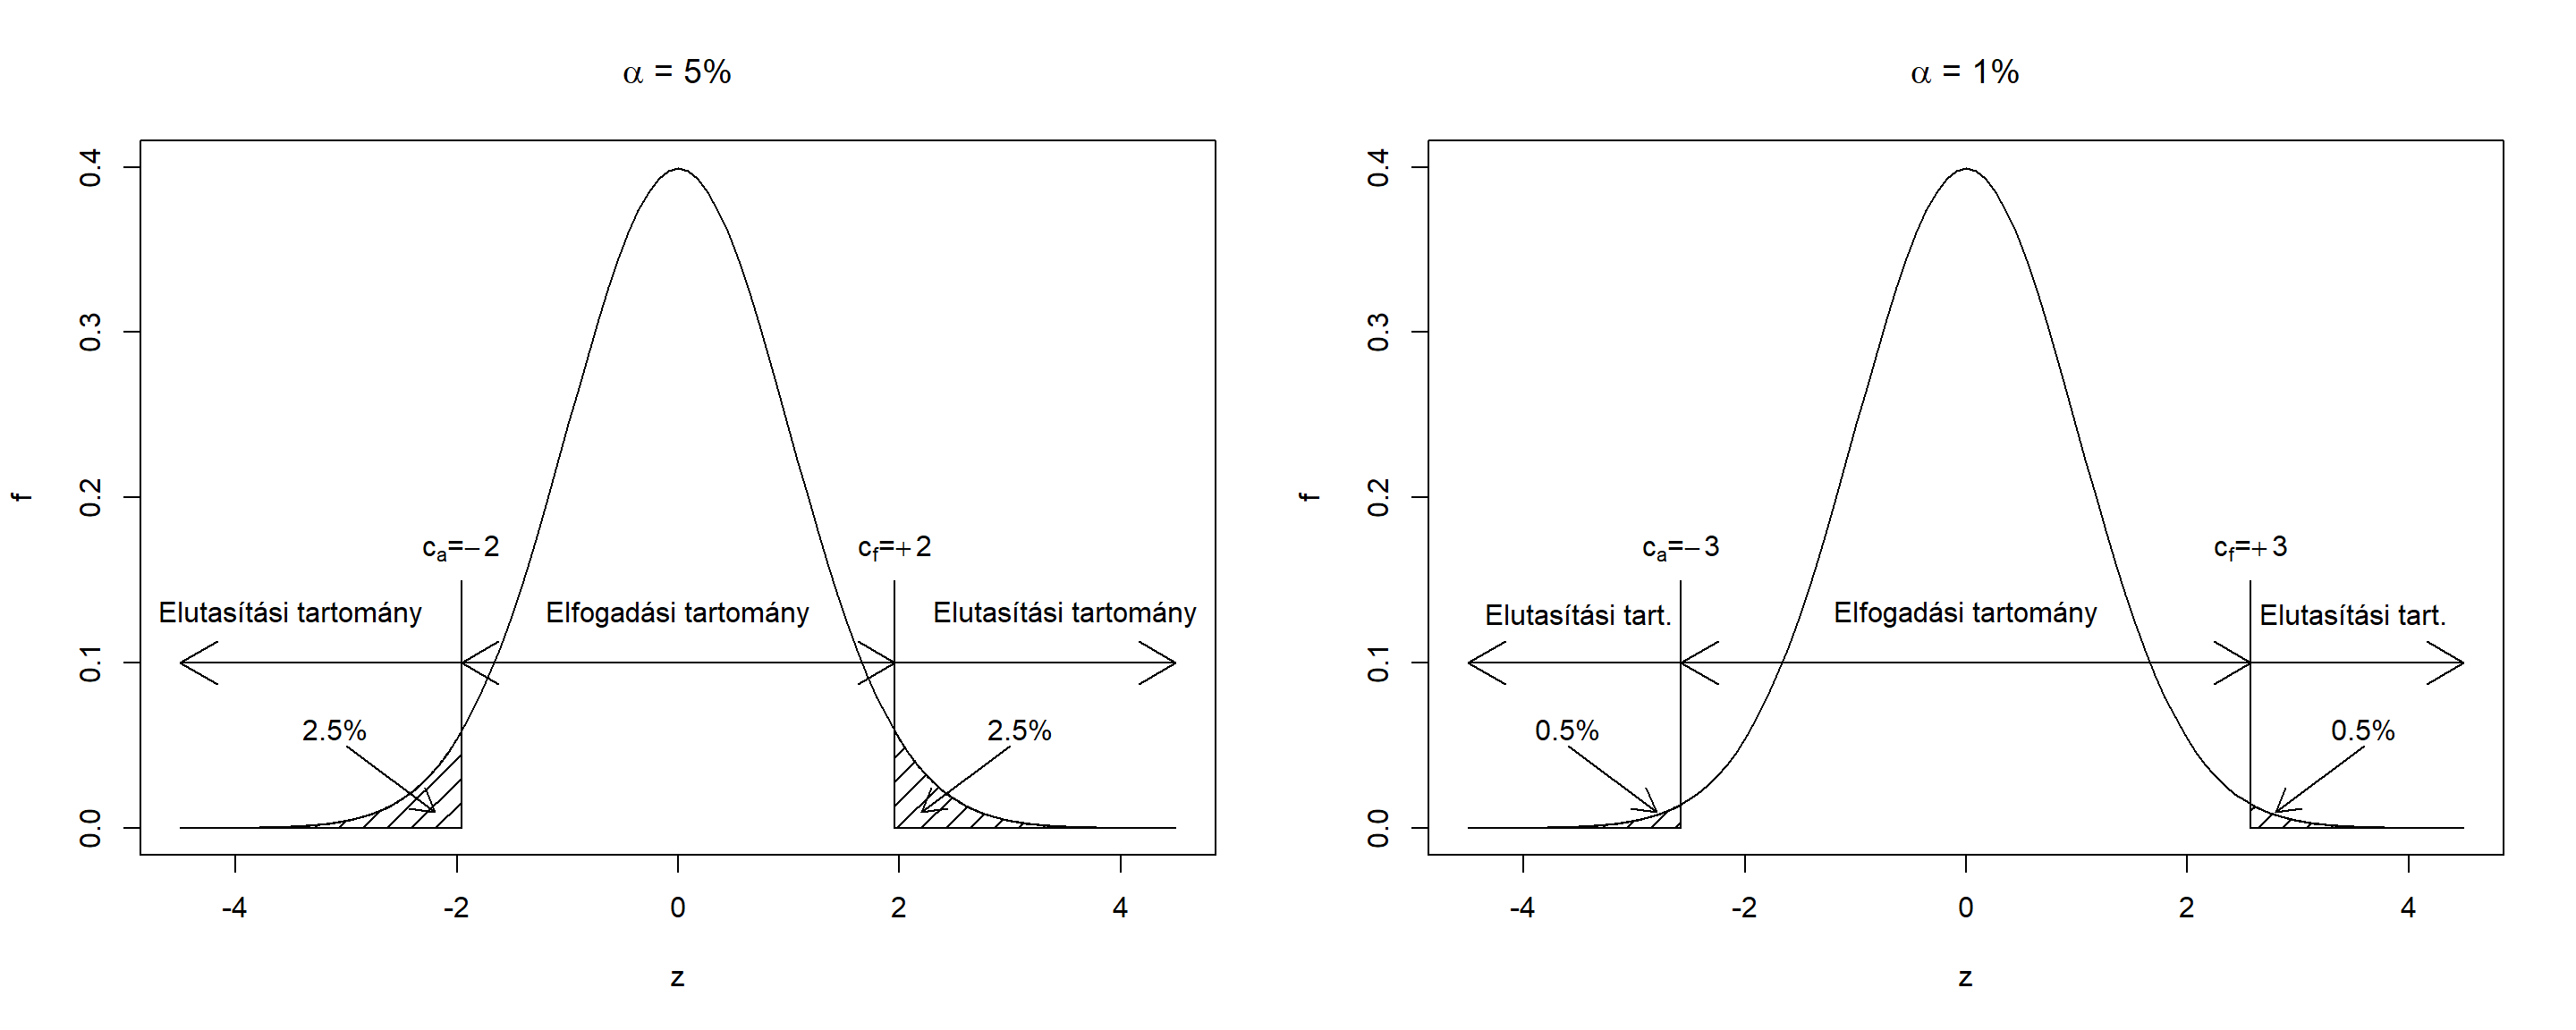
\includegraphics{bevbiostat_files/figure-latex/hiptartomanyok-1.pdf}
\caption{\label{fig:hiptartomanyok}A hipotézisvizsgálat döntésének
szemléltetése két szignifikanciaszint mellett.}
\end{figure}

Amint arra már utaltunk is, \(\alpha\) beállításával a
hipotézisvizsgálatban elkövethető kétféle hiba között egyensúlyozunk. Az
egyik tévedési lehetőség, hogy fennáll a nullhipotézis, mi mégis
elvetünk (ennek neve \textbf{elsőfajú hiba}; a valószínűsége felett
nagyon is erős kontrollunk van, hiszen az épp \(\alpha\)); a másik
hibázási lehetőség, hogy elvethetnénk a nullhipotézis, mi mégis
elfogadunk (ennek neve \textbf{másodfajú hiba}, a valószínűségét
\(\beta\)-val szokás jelölni; \(\beta\) értékét nem tudjuk jól kézben
tartani, hiszen attól is függ, hogy konkrétan milyen ellenhipotézis áll
fenn, amit általában mi sem tudhatunk). Ha \(\alpha\)-t növeljük
(,,beljebb húzzuk'`a kritikus értékeket, növeljük az elutasítási,
csökkentjük az elfogadási tartomány méretét), akkor megemeljük a téves
elutasítás, és lecsökkentjük a téves elfogadás valószínűségét, ha
\(\alpha\)-t csökkentjük (,,kijjebb toljuk'' a kritikus értékeket,
növeljük az elfogadási, csökkentjük az elutasítási tartomány méretét),
akkor megemeljük a téves elfogadás, és lecsökkentjük a téves elutasítás
valószínűségét. Az \(\alpha=5\)\% egy tipikus kompromisszum a kétféle
hibázás között. Kiegészítésként megjegyezzük, hogy
\(\left(1-\beta\right)\)-t a próba \textbf{erejének} szokás nevezni
(hiszen azt mutatja meg, hogy ha a valóságban nem áll fenn a
nullhipotézis, akkor azt mekkora valószínűséggel fogjuk detektálni).

A fentiekből is érezhető, hogy egy próba eredményének olyan formában
történő megadása, hogy ,,5\%-on szignifikáns'' nem a legszerencsésebb,
hiszen rögtön adódik a kérdés: vajon 1\%-on is szignifikáns lett volna?
És 0,1\%-on? Nem mindegy, hiszen egy olyan eredmény, mely 5\%-on
szignifikáns, de 4\%-on nem, sokkal nagyobb bizonytalanságú, mint egy
olyan, ami 0,1\%-on is szignifikáns. Megoldás lehetne a tesztstatisztika
konkrét értékének megadása, ez azonban gyakorlati szempontból nehézkes,
hiszen így minden esetben meg kéne nézni, hogy mi a nulleloszlás (hiszen
a tesztstatisztika empirikus értékét muszáj ahhoz viszonyítani). Éppen
ezért a mai gyakorlatban inkább azt adják meg, hogy \emph{melyik lenne}
az a szignifikanciaszint, ami mellett a tesztstatisztika empirikus
értéke épp az elutasítás és az elfogadás határa kerülne. Ennek neve:
\textbf{\(p\)-érték} (vagy empirikus szignifikanciaszint). Például,
gondoljuk azt, hogy próbánk 5\%-on elutasít. Ekkor elkezdjük az
\(\alpha\)-t csökkenteni (ezzel kijjebb húzzuk a kritikus értékeket,
bővítjük az elfogadási, szűkítjük az elutasítási tartomány). Elérjük a
4\%-ot, az empirikus tesztstatisztikánk még mindig az elutasítási
tartományban van, tovább csökkentjük az \(\alpha\)-t, és így
tovább\dots{} míg nem egyszer csak azt vesszük észre, hogy mondjuk
2,31\%-on még elutasít a teszt, de 2,29\%-on már nem. Ekkor azt mondjuk,
hogy a teszt \(p\)-értéke 2,3\%.

A \(p\)-érték tehát nem más, mint a szignifikanciaszint akkor, ha a
megfelelő (alsó vagy felső) kritikus értéket a tesztstatisztika
empirikus értékének helyére helyezzük át. (A másikat pedig,
értelemszerűen, az ellentétére, hiszen a kritikus értékek ebben ez
esetben -- ahogy már megbeszéltük -- szimmetrikusak.) Ebből az is
következik, hogy a \(p\)-érték számszerűen a nulleloszlás integrálja az
empirikus tesztstatisztikától extrémebb irányba (illetve ennek
kétszerese), ugyanúgy, ahogy az \(\alpha\) is -- definíció szerint -- a
nulleloszlás integrálja a kritikus értékektől extrémebb irányokba (és
itt, ahogy megbeszéltük, a kritikus érték szerepét az empirikus
tesztstatisztika játssza). Ennek meghatározása tehát manapság már
számítástechnikai szempontból is problémamentes.

Világos, hogy \(p\)-érték az elvetésben való bizonyosságunkat fejezi ki.
Ez az eredményközlés azért rendkívül praktikus, mert -- szemben az
előzőekkel -- az olvasó ,,elvégezheti magának'' a hipotézisvizsgálatot,
és \emph{bármilyen szignifikanciaszinten} döntést hozhat. A
\(p\)-értéknél magasabb szignifikanciaszinteken elutasítás lesz a döntés
(ekkor bővebb az elutasítási tartomány, bele fog esni az empirikus
tesztstatisztika), a \(p\)-értéknél alacsonyabb szinteken pedig
elfogadás (az elutasítási tartomány szűkebb, az empirikus
tesztstatisztika az elfogadási tartományba fog esni).

Végezetül egy fontos gyakorlati kérdésre hívjuk fel a figyelmet. Amint
már megbeszéltük, az \(\alpha\) azt mutatja meg, hogy egy adott próba
mekkora valószínűséggel ad téves jelzést. (Emlékezzünk rá, hogy
általában mi az elutasítást keressük!) Igen ám, de ha mi két próbát
végzünk egymástól függetlenül \emph{úgy}, hogy akkor is találatot
deklarálunk, ha \emph{legalább} az egyik teszt szignifikáns lett, akkor
valójában már \emph{nem} \(\alpha\) valószínűséggel kapunk jelzést akkor
is, ha nincs hatás (egyik esetben sem), hanem
\(1-\left(1-\alpha\right)^2\) valószínűséggel! (Hiszen a hibás jelzés
annak a komplementere, hogy mindkét teszt jó döntés ad, mivel pedig
függetlenek, ezek valószínűsége összeszorzódik.) Ez pedig nagyon nem
mindegy, a tipikus \(\alpha=5\)\%-ra ez a valószínűség már 9,75\%! Tehát
valójában majdnem a nominális szignifikanciaszint kétszerese lesz annak
a valószínűsége, hogy kapunk elutasítást -- miközben a valóságban nincs
is hatás egyik esetben sem! Ezt a jelenséget szokás
\(\alpha\)-inflációnak nevezni. (A kétféle \(\alpha\)-t pedig néha
megkülönböztetésül comparisonwise (\(\alpha_C\)) \(\alpha\)-nak illetve
familywise (\(\alpha_F\)) \(\alpha\)-nak nevezik. Az előbbi annak a
valószínűsége, hogy egy teszt hibás jelzést ad (ez az eddig tárgyalt
\(\alpha\)), az utóbbi annak a valószínűsége, hogy tesztek egy
családjából \emph{legalább egy} lesz, ami hibás jelzést ad.) Az
összefüggés a kettő között tehát: \[
    \alpha_F = 1-\left(1-\alpha_C\right)^k,
\] ahol \(k\) az elvégzett próbák száma.

Azt a helyzetet, amikor egymással párhuzamosan több, egymástól független
hipotézisvizsgálatot futtatunk (és vagylagosan keresünk szignifikáns
eredményt), \textbf{többszörös összehasonlítások helyzetének} szokás
nevezni.

A dolog azt sugallja számunkra, hogy ha sok tesztet végzünk
párhuzamosan, akkor valamit tenni kell az ellen, hogy ne találjuk túl
könnyen fals elutasításokat. A legegyszerűbb megoldás, ha a tesztenkénti
(comparisonwise) szignifikanciaszintet lecsökkentjük. Például, az ún.
Bonferroni-egyenlőtlenség szerint
\(1-\left(1-\alpha\right)^k\leq \alpha\cdot k\), ezért durva becsléssel
úgy korrigálhatjuk a szignifikanciaszintet, hogy elosztjuk a célszintet
az elvégzett hipotézisvizsgálatok számával. Ez garantálja, hogy a \(k\)
teszt elvégzését \emph{együttesen tekintve} sem lehet a kitűzött
szignifikanciaszint feletti az elsőfajú hibák aránya.

A módszer hátránya, hogy túl drasztikus: annyira megnehezíti a
nullhipotézis elvetését, hogy a valós különbségek is ,,el fognak
veszni''. Vannak módszerek, melyek ezt enyhítik (pl.
Holm--Bonferroni-korrekció), illetve melyek teljesen más elven próbálják
elérni az \(\alpha\)-infláció enyhítését (pl. FDR). Ennek a kérdéskörnek
például a microarray adatok kiértékelése kapcsán (ahol elképesztő
mennyiségű tesztet kell függetlenül végezni) nagyon megnőtt a
jelentősége; ettől eltekintve azonban az orvosok általában nem viszik
túlzásba a védekezést ez ellen\dots{}

Itt hívjuk fel a figyelmet az ún. \textbf{szignifikanciavadászat}
jelenségére. Ez lényegében nem más, mint a többszörös összehasonlítások
helyzetének rosszindulatú kiaknázása inkorrekt következtetésre. A
szignifikanciavadászat jelenségét inkább egy példával illusztráljuk:
tegyük fel, hogy bizonyítani akarjuk, hogy a hétfőn és kedden született
emberek laboreredményei között szignifikáns eltérés van. Bár ez
ránézésre látható módon abszurdum, a fentiek kihasználásával
tulajdonképpen nem is nehéz bizonyítani: manapság már a rutinszerűen
vizsgált laborparaméterek száma is eléri a 20-30-at, így nincs más
dolgunk, mint mindegyiket összehasonlítani! Természetesen valós
különbség sehol nem lesz, de mivel 5\% valószínűséggel mindegyik adhat
téves jelzést, így 30 között már az lenne a meglepő, ha nem kapnánk
egyetlen elutasítást sem. Ha a vizsgálatot -- korrekt módon -- úgy
publikáljuk le, hogy összehasonlítottunk 30 laborváltozót 5\%-on, és
közülük 1 esetben, az XYZ-nél szignifikáns különbséget találtunk, akkor
mindenki rögtön tudni fogja, hogy mi történt (azaz, hogy nem
jelenthetjük ki, hogy találtunk bármit is). Igen ám, de ha inkorrekt
módon játszunk, akkor azt tesszük, hogy a cikket úgy írjuk meg, hogy mi
\emph{előre} tudtuk, hogy XYZ-ben lesz különbség (mert van egy ragyogó
kórélettani modellünk, mely az XYZ termelését a születés napjával hozza
összefüggésbe), és ezért \emph{célirányosan} XYZ-t leteszteltük, és lám:
valóban szignifikáns különbséget is kaptunk\dots{}! Ezzel szemben nehéz
védekezni, hiszen magából az eredményközlésből nem lehet rájönni, hogy
mi történt (de természetesen a vizsgálat reprodukciója azonnal
lebuktatja a csalást).

Zárásként részletesebb indoklás nélkül felhívjuk három összefüggésre a
figyelmet.

\begin{enumerate}
\def\labelenumi{\arabic{enumi}.}
\tightlist
\item
  Nagyon fontos gyakorlati probléma, hogy adott feladat vizsgálatára
  konkrétan melyik próbát használjuk. Ez közel sem triviális kérdéskör,
  ugyanis a feladat önmagában még nem determinálja a próbát: sok feladat
  van, amire akár tucatnyi különböző próba is elérhető; ezek tipikusan
  az előfeltevéseikben különböznek. (Azaz, hogy milyen \emph{a priori}
  megkötésekkel élnek a sokaságra vonatkozóan.) Ennek kapcsán arra
  hívjuk fel a figyelmet, hogy egyrészt ha egy próba előfeltevései nem
  teljesülnek, de mi mégis alkalmazzuk, akkor nem garantált, hogy valid
  végeredményt kapunk, másrészt viszont a több előfeltevésre építő
  próbáknak általában kisebb az erejük. A tanulság, hogy mindig annyi
  előfeltevésre építő próbát használjunk, amennyit tudunk, se többet se
  kevesebbet: amely előfeltevésekről tudjuk, hogy teljesülnek (a
  priori!) azokat építsük be a próbaválasztásba\dots{} de többet ne.
\item
  Rögtön itt érdemes megjegyezni, hogy -- bár egyes statisztikai
  programcsomagok notóriusan az ellenkezőjét sugallják -- elvileg nem
  illik az alapján dönteni, hogy milyen próbát használunk, hogy az
  előfeltevéseit \emph{ugyanazon} mintán \emph{egy másik próbával}
  leellenőrizzük. Ezért hangsúlyoztuk az előbbi pontban, hogy a
  feltevésekről \emph{a priori} kell döntenünk (korábbi eredmény, másik
  mintán végzett teszt stb. alapján).
\item
  Végül felhívjuk a figyelmet, hogy egy próba erejét önmagában növeli a
  nagyobb mintanagyság. Pontosan ezért a klasszikus mondás szerint:
  ,,kis hatás kimutatásához nagy minta kell, nagy hatáshoz elég a kisebb
  minta is!''.
\end{enumerate}

Mutatunk egy példát a hipotézisvizsgálat alkalmazására is: vizsgáljuk
meg azt a kérdést, hogy a dohányzó anyák újszülötteinek születési tömege
eltér-e a nemdohányzó anyák újszülötteitől!

Az első kérdés, hogy mit értünk az alatt, hogy ,,eltér''. Ezt
többféleképp is lehetne operacionalizálni, most maradjunk annál a --
kézenfekvő, és klinikailag is releváns -- megközelítésnél, hogy a
várható születési tömegük kisebb-e. (Tehát a kérdést a várható értékek
egyezésére hegyezzük ki, nem az érdekel minket, hogy például a szórása a
születési tömegeknek eltér-e a két csoportban.)

Az adatbázisban 115 nemdohányzó és 74 dohányzó anyától származó
újszülött van. Gyorsan kiszámolhatjuk, hogy az előbbi csoportban az
újszülöttek átlagos születési tömege 3055,7 gramm, míg az utóbbiban
2771,9 gramm. Mondhatjuk akkor, hogy a dohányzó anyák újszülöttjei
kisebb tömegűek? Természetesen nem! Ez ugyanis csak annyit mondott, hogy
a \emph{mintában} kisebb a tömegük, de minket természetesen nem a
konkrét minta érdekel, hanem a sokaság! Kijelenthetjük ez alapján, hogy
a sokaságban is kisebb a dohányzó anyák újszülöttjeinek a várható
születési tömege? Nem, a helyzet nem ilyen egyszerű: elképzelhető, hogy
mindkét csoportnak ugyanannyi (a sokaságban!) a várható születési
tömege, csak épp pont olyan mintát vettünk, amiben a dohányzó anyáknál
ez kisebb. (Ez természetesen tökéletes mintavétel esetén is előfordulhat
-- mintavételi ingadozás, ugyebár!) Sőt, akár az is lehet, hogy épp a
dohányzó anyák újszülöttei nagyobb születési súlyúak várhatóan, csak a
mintavétel ördöge az ő csoportjukból pont kicsi, a nemdohányzó
csoportból meg nagyobb újszülötteket dobott ki.

A kérdésről tehát \emph{biztosat} nem lehet mondani -- de statisztikai
próbával \emph{valószínűségi kijelentést} tehetünk. Elsőként döntenünk
kell arról, hogy milyen próbát alkalmazzunk. Ennek a részletei számunkra
most nem fontosak, a lényeg csak a végeredmény: a körülmények (két
független csoport, aránylag nagy mintanagyság mindkét csoportban,
\emph{a priori} nem ismert sokasági szórás) a választásunk az ún.
Welch-próbára esik. Ennek nullhipotézise, hogy a két csoport várható
értéke között nincs különbség, ellenhipotézise, hogy van, a két várható
érték nem egyezik.

Elvégezve a próbát azt kapjuk, hogy a \(p\)-értéke: \(p=0,\!007003\).
Mivel ez a \(p\)-érték minden szokásos szignifikanciaszintnél kisebb
(még az 1\%-ot sem éri el), kijelenthetjük: a várható értékek egyezésére
vonatkozó nullhipotézis minden szokásos szignifikanciaszinten elvethető,
azaz minden szokásos szignifikanciaszinten kijelenthető, hogy a két
csoport (sokaságbeli!) várható értéke között különbség van. (Azaz: a
mintában tapasztalt különbség olyan nagy (a minta egyéb jellemzőit is
figyelembe véve), hogy az már túlmutat a mintavételi ingadozás hatásán,
nem hihető, hogy betudható pusztán a mintavételi ingadozás hatásának.
Azt kell feltételeznünk, hogy mögötte sokasági hatás (azaz sokaságban is
eltérő várható érték) van.)

Mindezt röviden úgy is megfogalmazhatjuk, hogy a különbség szignifikáns,
még más szóval, hogy a két csoport között lényeges különbség van. (Ebben
a kontextusban a ,,lényeges'`statisztikai értelemben szignifikánsat
jelent.) Ez a jó pont arra, hogy felhívjuk a figyelmet a különbségre a
-- most definiált -- \emph{statisztikai szignifikancia} és a -- köznapi
értelmű -- \emph{klinikai szignifikancia} között. E kettőt mindig
szigorúan különböztessük meg egymástól! A köznapi szóhasználatban a
,,lényeges különbség'' alatt ugyanis azt értjük, hogy a tárgyterületi
(esetünkben: orvosi) skálán mi bír jelentőséggel. 1 grammal nagyobb
születési tömegnek semmi (klinikai) jelentősége (nem gondol az orvos más
klinikai helyzetre, nem rendel más vizsgálat, más kezelést stb.), 500
grammnak nagyon is lehet. A statisztikai szignifikancia viszont
\emph{teljesen mást} mér: azt, hogy mennyire hihető, hogy a különbség
betudható a mintavételi ingadozásnak! Adott esetben lehet 500 gramm
különbség is (statisztikailag) inszignifikáns (ha nagy a szórás, vagy
kicsi a mintanagyság), és lehet 1 gramm különbség is (statisztikailag)
szignifikáns (ha kicsi a szórás, vagy nagy a mintanagyság).

Biztos ez a döntés? Természetesen nem! Bár a \(p\)-érték nagyon
alacsony, de mivel nem nulla (soha nem is lehet az), így épp azt
mutatja, hogy a döntésünkben mekkora bizonytalanság van -- mert van
benne.


\end{document}
